\documentclass[twoside,11pt]{article}

% Use JMLR style with preprint option
\usepackage[preprint]{jmlr2e}
\usepackage{amsmath}
\usepackage{bbm} 
% Additional packages (jmlr2e already includes: epsfig, amssymb, natbib, graphicx)
\usepackage{algorithm}
\usepackage{algorithmic}
\usepackage{subcaption}
\usepackage{xcolor}
\usepackage{tikz}
\usetikzlibrary{calc, arrows.meta, decorations.markings, patterns, shapes.geometric, positioning, 3d, decorations.pathmorphing}
\usepackage{array}
\usepackage{tabularx}
\usepackage{listings}
\lstset{basicstyle=\ttfamily, breaklines=true}
\usepackage{booktabs}

% Figure search paths (adjust for compilation directory)
\graphicspath{{./}{../../Transformer Manuscript/fig_transformer_validation/}}

% Note: jmlr2e already defines theorem environments and proof
% Available: theorem, lemma, proposition, corollary, definition, example
% Manual definitions (no amsmath needed)
\newcommand{\softmax}{\operatorname{softmax}}
\newcommand{\KL}{\operatorname{KL}}
\newcommand{\Tr}{\operatorname{Tr}}
\begin{document}

% JMLR heading for preprint
\jmlrheading{}{2025}{}{}{}{}{Robert C. Dennis}

\title{Attention, Transformers, and Backpropagation are\\
Degenerate Limits of the Variational Free Energy Principle}

\author{\name Robert C. Dennis \email cdenn016@gmail.com \\
       \addr Independent Researcher\\
       \addr Leander, Texas 78641, USA}

\editor{TBD}

\maketitle

\ShortHeadings{Attention and Transformers as Free Energy}{Dennis}
\begin{abstract}
We show that transformer attention is variational inference over information sources. Modeling each token as a Gaussian agent on a statistical fiber bundle, we derive the generalized attention weight $\beta_{ij} = \operatorname{softmax}(-D_{\mathrm{KL}}[q_i \| \Omega_{ij} q_j] / \tau)$ from a single variational principle: minimizing the free energy of a mixture-of-sources generative model in which each agent infers, via gauge transport, which neighbor generated its state. The KL divergence arises exactly and the softmax follows from constrained optimization over the categorical source-selection posterior.

From this single principle, several transformer architectural choices typically emerge as consequences of this variational geometry: the temperature scaling $1/\sqrt{d_k}$ from dimensional concentration of the KL divergence, layer normalization as the geometric condition for frame-independent inference, multi-head attention as a block-diagonal restriction of the gauge algebra, and causal masking and positional biases from non-uniform attention priors $\pi_j$. Taking two limits of this framework (isotropic covariances, flat gauge connection) recovers the standard rule $\beta_{ij} \propto \operatorname{softmax}(Q_i K_j^\top / \sqrt{d_k})$. The $\mathrm{GL}(K)$ invariance of KL divergence further implies that $W_Q, W_K$ are themselves gauge transformations with $\Omega = W_Q W_K^\top$ a learned gauge transport. Standard transformers therefore already implement gauge-theoretic attention. Gradient descent on the free energy recovers backpropagation and learning, providing a variational interpretation of transformer training.

We validate the degenerate-limit predictions on a frozen BERT model across 105 diverse passages, confirming quantitative agreement between KL-based and dot-product attention (grand mean $r = 0.804$ at the predicted optimal temperature, 95\% CI $[0.771, 0.838]$, with cross-passage SE $< 0.02$ for all 144 heads). We further validate the full unreduced theory by training a $\mathrm{GL}(K)$ gauge transformer on WikiText-103 using only KL divergences, geometry, and gauge transport without any learned attention projections, MLPs, or activation functions. The model achieves test perplexity 121 with emergent semantic structure in the learned gauge frames and beliefs.
\end{abstract}

\noindent\textbf{Keywords:} gauge theory, free energy principle, transformer attention, variational inference, information geometry, natural gradient, symmetry breaking, multi-agent systems, $\mathrm{GL}(K)$ invariance

\section{Introduction}

Language is fundamentally a dynamic informational system: speakers and writers encode beliefs under uncertainty, listeners decode them, and the statistical regularities of this process reflect the structure of communication itself. Language modeling---predicting the next token given context---is a snapshot of this dynamic system, and the architectures that excel at it should reflect the mathematical structure of information exchange under uncertainty.

Recent advances in neuroscience and intelligent systems have independently converged on the idea that intelligent systems integrate perception, inference, and communication under the constraints of uncertainty \citep{bahdanau2014neural,amari1998natural,bronstein2021geometric,foerster2016learning,wooldridge2009introduction}. Friston's Free Energy Principle (FEP) provides a general variational formulation of inference in cognitive systems \citep{friston2010free,parr2022active,friston2017graphical,ramstead2020variational}, whereas the attention mechanism in modern machine learning architectures defines a powerful (although empirically derived) rule for token prediction \citep{clark2019does,vaswani2017attention}. Despite their shared reliance on probabilistic inference and pairwise interaction, these two frameworks remain stubbornly separated. In particular, transformer attention lacks an underlying geometric or mathematical foundation and details on how and why modern machine learning architectures operate as well as they do remains obscure.

Many varieties of transformer and attention architectures have been proposed, implemented, and studied in recent years \citep{fuchs2020se3,thomas2018tensor}. Some architectures make use of bundle geometric frameworks but lack a first-principles foundation or connection to the FEP \citep{kondor2018generalization,finzi2020generalizing,bronstein2021geometric}. Furthermore, attempts at curved space token embeddings have produced mixed results \citep{bonnabel2013stochastic,absil2008optimization}.

Several complementary mathematical perspectives on attention have been developed. \citet{tsai2019transformer} and \citet{katharopoulos2020transformers} interpret attention through the lens of kernel methods, showing that softmax attention approximates a kernel function and can be linearized. \citet{ramsauer2021hopfield} demonstrate that attention implements the update rule of modern Hopfield networks, providing an energy-based perspective. The information bottleneck principle \citep{tishby2015deep,shwartz2017opening} offers a related information-theoretic view of layer-wise representation learning. On the side of backpropagation-free learning, \citet{hinton2022forward} proposes the forward-forward algorithm as an alternative to backpropagation. In neuroscience, predictive coding \citep{rao1999predictive,bogacz2017tutorial,millidge2021predictive} implements variational free energy minimization through local prediction errors, sharing the variational foundation of our framework but lacking the gauge-theoretic structure that connects to attention mechanisms. Our work differs from these approaches in providing a unified geometric framework from which attention, temperature scaling, layer normalization, and training dynamics all emerge as consequences of a single variational principle on a statistical fiber bundle.

In this report we propose a first-principles, gauge-equivariant framework that connects these domains. Our framework is based on a principal bundle geometry whereby each agent is modeled as a smooth local section of an associated bundle with statistical manifold fibers over a "noumenal" base manifold. Inter-agent communication arises naturally through a (generally) non-abelian gauge connection that defines parallel-transport operators between agents' local gauge frames. Within this geometry, attention emerges as a gauge-aligned Kullback–Leibler (KL) term derived directly from the variational free energy of a coupled multi-agent generative model based on mixture Gaussians.

We then show that in the flat-bundle, isotropic, delta-function limit attention reduces to the standard transformer dot-product attention $QK^T$, thereby identifying attention as a degenerate case of a broader geometric and statistical law of communication predicated upon the FEP and information geometry.  We demonstrate this by training a transformer based upon variational gradient descent of a generalized free energy of multivariate Gaussian agents as well as by applying our gauge attention theory to a frozen transformer (BERT) across a corpus of 105 diverse passages, with cross-passage validation confirming the robustness of our predictions.  We then describe numerical results that suggest that token encoding under data training (i.e. agent/token belief alignment) is a symmetry breaking phenomenon of our gauge-theoretic framework.

Finally, we show that gradient descent on the gauge-equivariant free energy, in the deterministic constant-gauge limit, recovers the standard transformer training update. This provides a variational interpretation of backpropagation: the chain rule through layered compositions corresponds to variational message-passing in the gauge-theoretic framework. The framework naturally invokes natural gradient descent on the Fisher-Rao metric, which offers theoretical convergence advantages; whether this translates to practical speedup in deep learning requires controlled empirical comparison, which we leave to future work.

\subsection{An intuitive simplification for non-geometers}
For interdisciplinary readers, it may be helpful to visualize each agent in this framework as a vector and a matrix field defined over a finite spatial region. 

Concretely, at every point $c$ in the base manifold, agent $i$ carries a mean vector $\mu_i(c)$ and a covariance matrix $\Sigma_i(c)$ representing, respectively, its local expected state and uncertainty. Together these form a smooth Gaussian field—the agent’s belief section of the statistical bundle. 

We will see that the agent's local gauge frame $\phi_i(c)$ may be intuitively interpreted as the agent's subjective frame of reference; its internal coordinate system through which beliefs and models are represented and compared. In this sense, $\phi_i(c)$ captures an agent’s “internal orientation” toward the world: it determines how external information is projected into the agent’s internal representational space. Gauge transformations $\phi_i(c) \to \phi_i(c) + \xi(c)$ thus correspond to changes in perspective that leave the underlying informational content invariant, much like shifts of viewpoint in perception that preserve the same world model. 

\begin{figure}[h]
\centering
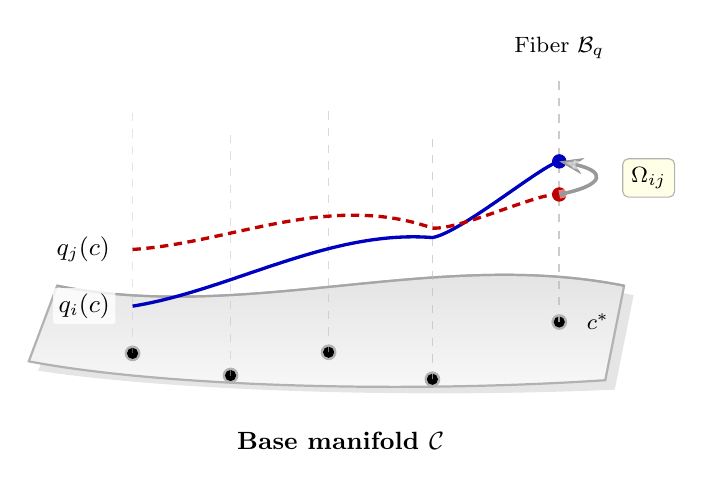
\begin{tikzpicture}[scale=1.2, every node/.style={font=\small}]
% requires \usetikzlibrary{calc, arrows.meta, decorations.markings, shadows}

% ------------------------------------------------------------------
% ENHANCED 3D BASE MANIFOLD with gradient and shadow
% ------------------------------------------------------------------
\path
  (0,0) coordinate (M1)
  (6,0) coordinate (M2)
  (5.8,-1.0) coordinate (M3)
  (-0.3,-0.8) coordinate (M4);

% Shadow layer
\filldraw[fill=black!10, draw=none]
  ($(M1)+(0.1,-0.1)$)
    .. controls (2.1,-0.5) and (4.1,0.3) .. ($(M2)+(0.1,-0.1)$)
    -- ($(M3)+(0.1,-0.1)$)
    .. controls (3.6,-1.2) and (1.1,-1.1) .. ($(M4)+(0.1,-0.1)$)
    -- cycle;

% Main surface with gradient
\shade[top color=gray!25, bottom color=gray!5, draw=gray!60, thick]
  (M1)
    .. controls (2,-0.4) and (4,0.4) .. (M2)
    -- (M3)
    .. controls (3.5,-1.15) and (1.0,-1.05) .. (M4)
    -- cycle;

% Surface outline for crispness
\draw[gray!70, thick]
  (M1)
    .. controls (2,-0.4) and (4,0.4) .. (M2);

\node[below, black, font=\small\bfseries] at (3,-1.45) {Base manifold $\mathcal{C}$};

% ------------------------------------------------------------------
% FIBER ANCHOR POINTS with improved positioning
% ------------------------------------------------------------------
\coordinate (C1) at ($(M4)!0.18!(M3)+(0,0.12)$);
\coordinate (C2) at ($(M4)!0.35!(M3)+(0,-0.08)$);
\coordinate (C3) at ($(M4)!0.52!(M3)+(0,0.20)$);
\coordinate (C4) at ($(M4)!0.70!(M3)+(0,-0.05)$);
\coordinate (C5) at ($(M4)!0.92!(M3)+(0,0.60)$);

% Anchor points with subtle glow
\foreach \c in {C1,C2,C3,C4,C5} {
  \filldraw[black!30] (\c) circle (2.2pt);
  \filldraw[black] (\c) circle (1.5pt);
}

% ------------------------------------------------------------------
% FIBERS with gradient opacity for depth
% ------------------------------------------------------------------
\foreach \c [count=\i] in {C1,C2,C3,C4,C5} {
  \pgfmathsetmacro{\opacity}{0.3 + \i*0.1}
  \draw[gray!50, dashed, line width=0.6pt, opacity=\opacity] 
    (\c) -- ++(0,2.6);
}

% Fiber label with better positioning
\node[above=3pt, black, font=\footnotesize] at ($(C5)+(0,2.6)$) {Fiber $\mathcal{B}_q$};

% ------------------------------------------------------------------
% SECTION CURVES with enhanced styling
% ------------------------------------------------------------------
% Section q_i (solid blue)
\draw[thick, blue!75!black, line width=1.2pt]
  ($(C1)+(0,0.5)$)
    .. controls ($(C2)+(0,0.9)$) and ($(C3)+(0,1.3)$)
    .. ($(C4)+(0,1.5)$)
    .. controls ($(C4)+(0.3,1.55)$) and ($(C5)+(-0.2,1.65)$)
    .. ($(C5)+(0,1.7)$);

% Section q_j (dashed red)
\draw[thick, red!75!black, densely dashed, line width=1.2pt]
  ($(C1)+(0,1.1)$)
    .. controls ($(C2)+(0,1.4)$) and ($(C3)+(0,1.7)$)
    .. ($(C4)+(0,1.6)$)
    .. controls ($(C4)+(0.3,1.58)$) and ($(C5)+(-0.2,1.38)$)
    .. ($(C5)+(0,1.35)$);

% Enhanced section labels with background
\node[left=6pt, black, fill=white, fill opacity=0.8, text opacity=1, 
      inner sep=2pt, rounded corners=1pt] 
  at ($(C1)+(0,0.5)$) {$q_i(c)$};
\node[left=6pt, black, fill=white, fill opacity=0.8, text opacity=1, 
      inner sep=2pt, rounded corners=1pt] 
  at ($(C1)+(0,1.1)$) {$q_j(c)$};

% Section endpoint markers
\filldraw[blue!75!black] ($(C5)+(0,1.7)$) circle (2pt);
\filldraw[red!75!black]  ($(C5)+(0,1.35)$) circle (2pt);

% Highlight the special point c*
\node[right=3pt, black, font=\footnotesize\itshape] 
  at ($(C5)+(0.1,0)$) {$c^*$};

% ------------------------------------------------------------------
% TRANSPORT OPERATOR with improved arrow
% ------------------------------------------------------------------
\draw[-{Stealth[length=3mm, width=2mm]}, very thick, black!80, 
      line width=1.3pt,
      postaction={draw, line width=3pt, white, opacity=0.5, -{Stealth[length=3mm, width=2mm]}}]
  ($(C5)+(0,1.35)$)
    .. controls ($(C5)+(0.5,1.45)$) and ($(C5)+(0.5,1.60)$)
    .. ($(C5)+(0,1.7)$);

% Transport label with background box
\node[right=5pt, black, fill=yellow!10, draw=black!30, 
      inner sep=3pt, rounded corners=2pt, font=\footnotesize\bfseries] 
  at ($(C5)+(0.52,1.525)$) {$\Omega_{ij}$};

\end{tikzpicture}
\caption{%
Visualization of agent sections $q_i(c)$ and $q_j(c)$ over an associated bundle. 
The shaded surface represents the base manifold $\mathcal{C}$, with vertical fibers $\mathcal{B}_q$ 
shown as dashed lines anchored at black points. 
At the reference point $c^*$ on the rightmost fiber, the transport operator $\Omega_{ij}(c^*)$ 
maps the red section value $q_j(c^*)$ into the blue section value $q_i(c^*)$, 
enabling frame alignment between agent representations.
}
\label{fig:bundle_sections_surface}
\end{figure}


\section{Methods}

We begin with a general geometric construction that naturally supports hierarchical emergence of meta-agents, scale interactions, and non-trivial holonomy of transport. The details of the most general geometry and framework can be found in the appendix and references \citep{nakahara2003geometry,kullback1951information,sternberg1994group,fulton1991representation,frankel2011geometry,baez1994gauge}.  

Briefly, in this current report, we describe agents as modeled by a local section of an associated bundle to a principal $G$ fiber bundle whereby tokens are represented by agents occupying a single 0-dimensional base manifold with no particular ordering. We shall show that this framework enables a unified description of both intra-agent inference and inter-agent communication in terms of gauge frame transport and alignment via a generalized free energy principle. 


\subsection{Specializations for the Current Study}
Here we specify the simplifications adopted for the remainder of this work, which retain essential geometric structure while ensuring computational tractability and simplification.

\subsubsection{Matched Bundles}
In our general formulation agents are treated as pairs of sections of associated bundles $\mathcal{B}_q$ and $\mathcal{B}_p$ of beliefs and models.  Here we simplify by implementing

\begin{equation}
\mathcal{B}_q = \mathcal{B}_p =: \mathcal{B}, \qquad \rho_q = \rho_p =: \rho.
\end{equation}

This gives $\mathcal{E}_q = \mathcal{E}_p =: \mathcal{E}$, and the bundle morphisms become:

\begin{equation}
\Phi = \tilde{\Phi} = \text{id}_{\mathcal{E}}.
\end{equation}

Each agent then reduces to a single section $\sigma^i: \mathcal{U}_i \to \mathcal{E}$, with belief/prior distinction maintained through local fiber coordinates.



\subsubsection{Gauge Group and Representations}
The natural gauge group for KL-based attention is $G = \mathrm{GL}(K)$, the general linear group of invertible $K \times K$ matrices. This acts on the fibers via representations:

\begin{equation}
\rho_q: \mathrm{GL}(K) \to \mathrm{GL}(d_q),
\qquad
\rho_p: \mathrm{GL}(K) \to \mathrm{GL}(d_p).
\label{eq:representations}
\end{equation}

For $\Omega \in \mathrm{GL}(K)$, the gauge action on a Gaussian state is:

\begin{equation}
\boxed{
\begin{aligned}
\rho_q(\Omega) \cdot (\mu_q, \Sigma_q)
&= \big(\rho_q(\Omega)\,\mu_q,\;
\rho_q(\Omega)\,\Sigma_q\,\rho_q(\Omega)^\top\big),\\
\rho_p(\Omega) \cdot (\mu_p, \Sigma_p)
&= \big(\rho_p(\Omega)\,\mu_p,\;
\rho_p(\Omega)\,\Sigma_p\,\rho_p(\Omega)^\top\big).
\end{aligned}
}
\label{eq:gauge_action_gaussians}
\end{equation}

By Theorem~\ref{thm:glk_invariance}, KL divergence is invariant under this action for any $\Omega \in \mathrm{GL}(K)$. The only requirement is invertibility ($\det \Omega \neq 0$), not orthogonality. (Since our transport operators are parameterized via the matrix exponential, their determinants are always positive; see Remark~\ref{rem:exp_surjectivity}.)







\begin{table}[h]
\centering
\renewcommand{\arraystretch}{1.2}
\setlength{\tabcolsep}{6pt}
\begin{tabularx}{\textwidth}{lXX}
\hline
\textbf{Property} &
\textbf{Full Gauge Theory} &
\textbf{Standard Transformer} \\
\hline
Gauge group $G$ &
$\mathrm{GL}(K)$ or subgroup &
$\mathrm{GL}(d_k)$ (implicit) \\
Gauge transformation &
$\Omega_{ij} = e^{\phi_i} e^{-\phi_j} \in \mathrm{GL}^+(K)$ &
$\Omega = W_Q W_K^\top$ (learned, constant) \\
Frame field $\phi_i(c)$ &
Varies per agent/position &
Absorbed into $W_Q, W_K$ \\
Transport structure &
Agent-pair dependent &
Uniform across all pairs \\
Connection $A_\mu$ &
$-\partial_\mu \phi_i \neq 0$ &
$0$ (flat connection) \\
Curvature $F_{\mu\nu}$ &
Can be $\neq 0$ &
$0$ (trivial holonomy) \\
KL coupling &
$D_{\text{KL}}[q_i \,\|\, \Omega_{ij} q_j]$ &
$D_{\text{KL}}[q_i \,\|\, \Omega q_j]$ with constant $\Omega$ \\
What is learned &
Frame fields $\phi_i$ &
Global gauge $W_Q, W_K$ \\
\hline
\end{tabularx}
\caption{Comparison between full gauge-theoretic formulation and standard transformers.}
\label{tab:gauge_vs_transformer}
\end{table}





\subsubsection{Local Gauge Frames}
Each agent $i$ has a gauge frame field $\phi_i: \mathcal{U}_i \to \mathfrak{gl}(K)$ which may vary spatially.  This induces a local connection:

\begin{equation}
A^{(i)}_\mu(c) = -\partial_\mu \phi_i(c) + \mathcal{O}(\phi_i^2),
\end{equation}

with field strength:

\begin{equation}
F^{(i)}_{\mu\nu}(c) = \partial_\mu A^{(i)}_\nu - \partial_\nu A^{(i)}_\mu + [A^{(i)}_\mu, A^{(i)}_\nu].
\end{equation}

In the 0-dimensional case, which we consider here, there exist no gauge connections $A_\mu$ or field strengths $F_{\mu\nu}$. What remains is the algebraic structure of group-valued frame transformations $\Omega_{ij} = \exp(\phi_i)\exp(-\phi_j)$ acting on statistical fibers. This algebraic structure already suffices to recover transformer attention (as shown below), and already provides a functional language model when implemented without taking the degenerate limits (Section~\ref{sec:glk_lm}). The richer differential-geometric content is available in the full theory on higher-dimensional base manifolds and represents a direction for future work (see Section~6.3).


\subsubsection{Gauge-Aligned Divergence}
With these assumptions, the gauge-aligned KL divergence between agents is (see appendix):

\begin{equation}
D_{\text{KL}}\left[q_i(c) \,\big\|\, \Omega_{ij}(c) q_j(c)\right],
\end{equation}

where for Gaussian beliefs:

\begin{equation}
\Omega_{ij}(c) \cdot (\mu_j, \Sigma_j) = \left(\Omega_{ij}(c)\mu_j, \, \Omega_{ij}(c)\Sigma_j\Omega_{ij}(c)^\top\right).
\end{equation}

This divergence forms the basis of our attention mechanism.

\subsubsection{$\mathrm{GL}(K)$ Gauge Invariance of KL Divergence}
\label{sec:glk_invariance}

A key observation underlying our framework is that the Kullback-Leibler divergence possesses a maximal gauge symmetry: it is invariant under the full general linear group $\mathrm{GL}(K)$. This is a standard result in information geometry (see, e.g., \citet{amari2016information}), but its implications for transformer attention have not been previously recognized. We state it here for completeness.

\begin{theorem}[$\mathrm{GL}(K)$ Gauge Invariance]
\label{thm:glk_invariance}
For any two Gaussian distributions $P = \mathcal{N}(\mu_P, \Sigma_P)$ and $Q = \mathcal{N}(\mu_Q, \Sigma_Q)$ on $\mathbb{R}^K$, and any invertible linear transformation $\Omega \in \mathrm{GL}(K)$, the KL divergence is invariant under simultaneous pushforward:
\begin{equation}
D_{\mathrm{KL}}(\Omega_* P \,\|\, \Omega_* Q) = D_{\mathrm{KL}}(P \,\|\, Q),
\label{eq:glk_invariance}
\end{equation}
where $\Omega_* P = \mathcal{N}(\Omega\mu_P, \Omega\Sigma_P\Omega^\top)$ denotes the pushforward of $P$ under $\Omega$.
\end{theorem}

\begin{proof}
The KL divergence between Gaussians consists of three terms:
\begin{equation}
D_{\mathrm{KL}}(P \| Q) = \frac{1}{2}\left[\mathrm{Tr}(\Sigma_Q^{-1}\Sigma_P) + (\mu_P - \mu_Q)^\top \Sigma_Q^{-1}(\mu_P - \mu_Q) - K + \log\frac{\det\Sigma_Q}{\det\Sigma_P}\right].
\end{equation}

Under the pushforward $\Omega_* P = \mathcal{N}(\Omega\mu_P, \Omega\Sigma_P\Omega^\top)$ and $\Omega_* Q = \mathcal{N}(\Omega\mu_Q, \Omega\Sigma_Q\Omega^\top)$:

\textbf{Trace term:}
\begin{equation}
\mathrm{Tr}\big[(\Omega\Sigma_Q\Omega^\top)^{-1}(\Omega\Sigma_P\Omega^\top)\big] = \mathrm{Tr}\big[\Omega^{-\top}\Sigma_Q^{-1}\Omega^{-1}\Omega\Sigma_P\Omega^\top\big] = \mathrm{Tr}(\Sigma_Q^{-1}\Sigma_P). \quad \checkmark
\end{equation}

\textbf{Quadratic term:}
\begin{align}
&(\Omega\mu_P - \Omega\mu_Q)^\top (\Omega\Sigma_Q\Omega^\top)^{-1} (\Omega\mu_P - \Omega\mu_Q) \nonumber\\
&= (\mu_P - \mu_Q)^\top \Omega^\top \Omega^{-\top}\Sigma_Q^{-1}\Omega^{-1}\Omega (\mu_P - \mu_Q) = (\mu_P - \mu_Q)^\top \Sigma_Q^{-1}(\mu_P - \mu_Q). \quad \checkmark
\end{align}

\textbf{Log-determinant term:}
\begin{equation}
\log\frac{\det(\Omega\Sigma_Q\Omega^\top)}{\det(\Omega\Sigma_P\Omega^\top)} = \log\frac{(\det\Omega)^2 \det\Sigma_Q}{(\det\Omega)^2 \det\Sigma_P} = \log\frac{\det\Sigma_Q}{\det\Sigma_P}. \quad \checkmark
\end{equation}

The $(\det\Omega)^2$ factors cancel identically. Since all three components are invariant, $D_{\mathrm{KL}}(\Omega_* P \| \Omega_* Q) = D_{\mathrm{KL}}(P \| Q)$.
\end{proof}

Importantly, the proof extends to all $f$-divergences: for any convex function $f$ with $f(1) = 0$,

\begin{equation}
D_f(\Omega_* P \| \Omega_* Q) = D_f(P \| Q), \quad \forall\, \Omega \in \mathrm{GL}(K),
\end{equation}

since the Jacobian factors $|\det\Omega|$ from the density transformation cancel in the ratio $p(x)/q(x)$. From a practical point of view, this means that transport operators need only satisfy $\det(\Omega_{ij}) \neq 0$ (invertibility); the full $\mathrm{GL}(K)$ acts as a gauge symmetry. Our exponential parameterization restricts to $\det > 0$ (see Remark~\ref{rem:exp_surjectivity}), but this is the identity component and is standard for gauge connections. Finally, we shall demonstrate that the query and key projection matrices $W_Q, W_K \in \mathrm{GL}(d_k)$ in standard transformers are themselves gauge transformations. The constant gauge limit corresponds not to the absence of gauge structure, but to a constant gauge transformation $\Omega = W_Q W_K^\top$ shared among all token pairs.


\begin{table}[h]
\centering
\renewcommand{\arraystretch}{1.15}
\setlength{\tabcolsep}{6pt}
\begin{tabularx}{\textwidth}{l>{\raggedright\arraybackslash}Xl}
\hline
\textbf{Symbol} & \textbf{Description} & \textbf{Type/Dimension} \\
\hline
\multicolumn{3}{l}{\textit{Fiber Bundle Structure}} \\
$\mathcal{C}$ & Base manifold (spatial domain) & Manifold \\
$\mathcal{B}_q$ & Belief fiber & $\mathbb{R}^{K_q}$ \\
$\mathcal{B}_p$ & Model fiber  & $\mathbb{R}^{K_p}$ \\
$G$ & Gauge group & $\mathrm{GL}(K)$ \\
$\mathfrak{g}$ & Lie algebra of $G$ & $\mathfrak{gl}(K)$ \\
\\
\multicolumn{3}{l}{\textit{Gauge Fields and Connections}} \\
$\Omega_{ij}$ & Connection $\mathcal{B}_{q_j} \to \mathcal{B}_{q_i}$ & $\mathrm{GL}(K_q)$ \\
$\tilde\Omega_{ij}$ & Connection $\mathcal{B}_{p_j} \to \mathcal{B}_{p_i}$ & $\mathrm{GL}(K_p)$ \\
$\phi_i$ & Gauge parameter (belief frame) & $\mathfrak{g}\!\cong\!\mathbb{R}^3$ \\
$\tilde{\phi}_i$ & Gauge parameter (model frame) & $\mathfrak{g}\!\cong\!\mathbb{R}^3$ \\

\\
\multicolumn{3}{l}{\textit{Bundle Morphisms}} \\
$\Phi_i$ & Morphism $\mathcal{B}_{q_i} \to \mathcal{B}_{p_i}$ & $\mathbb{R}^{K_p\times K_q}$ \\
$\tilde{\Phi}_i$ & Morphism $\mathcal{B}_{p_i} \to \mathcal{B}_{q_i}$ & $\mathbb{R}^{K_q\times K_p}$ \\
\\
\multicolumn{3}{l}{\textit{Statistical Parameters}} \\
$q_i(k_i)$ & Belief distribution & $\mathcal{N}(\mu_{q,i},\Sigma_{q,i})$ \\
$p_i(k_i)$ & Model distribution & $\mathcal{N}(\mu_{p,i},\Sigma_{p,i})$ \\
$\mu_{q,i},\mu_{p,i}$ & Mean vectors & $\mathbb{R}^{K_q},\mathbb{R}^{K_p}$ \\
$\Sigma_{q,i},\Sigma_{p,i}$ & Covariance matrices & $\mathbb{R}^{K\times K},\succ0$ \\
\\
\multicolumn{3}{l}{\textit{Attention and Coupling}} \\
$\beta_{ij}$ & Belief Attention weight $j\!\to\!i$ & $[0,1]$ \\
$\gamma_{ij}$ & Model Attention weight $j\!\to\!i$ & $[0,1]$ \\
$\tau$ & Attention temperature & $\mathbb{R}_+$ \\
$\alpha_i$ & State-dependent self-consistency strength (Sec.~\ref{sec:state_dependent_precision}) & $\mathbb{R}_+$ \\
$D_{\mathrm{KL}}$ & Kullback–Leibler divergence & $\mathbb{R}_+\cup\{0\}$ \\
\hline
\end{tabularx}
\caption{Notation used throughout this paper.}
\label{tab:notation}
\end{table}



\section{Gauge-Covariant Variational Free Energy}
\label{sec:free_energy_section}

We now construct the variational free energy for a multi-agent system coupled by gauge transport. All probability distributions are defined at a specific base manifold point $c = c^*$ unless otherwise noted. We label the fiber's latent coordinates as $k_i \in \mathcal{B}$ in order to define the necessary integrals.

\subsection{Agent State Space}

Each agent $i$ maintains two distinct latent variables living in separate fiber bundles:

\begin{equation}
k_i \in \mathbb{R}^{K_q} \quad \text{(belief latent in $\mathcal{E}_q$)},
\qquad
m_i \in \mathbb{R}^{K_p} \quad \text{(model latent in $\mathcal{E}_p$)}.
\label{eq:dual_latents}
\end{equation}

The full state of agent $i$ is taken to be a multi-variate Gaussian (MVG) distribution over each latent:

\begin{equation}
\begin{aligned}
q_i(k_i) &= \mathcal{N}(k_i\,;\mu_{q,i},\,\Sigma_{q,i}),
\quad \Sigma_{q,i} \succ 0,\\
s_i(m_i) &= \mathcal{N}(m_i\,;\mu_{p,i},\,\Sigma_{p,i}),
\quad \Sigma_{p,i} \succ 0.
\end{aligned}
\label{eq:gaussian_states}
\end{equation}

Each latent has an independent Gaussian base prior encoding agent-specific inductive biases:

\begin{equation}
p_i(k_i) = \mathcal{N}(k_i\,; \mu_{0,i}^{(q)}, \Sigma_{0,i}^{(q)}),
\qquad
r_i(m_i) = \mathcal{N}(m_i\,; \mu_{0,i}^{(p)}, \Sigma_{0,i}^{(p)}).
\label{eq:base_priors}
\end{equation}

These priors are local in that they live within each agent's own gauge frame $\phi$ and need not be related across agents until transported via the gauge connection.

\subsection{Gauge Transport}

The gauge transport operators $\Omega_{ij}, \tilde{\Omega}_{ij}$ are pointwise gauge frame transformations:

\begin{equation}
\Omega_{ij}(c) = e^{\phi_i(c)} \cdot e^{-\phi_j(c)} \in \mathrm{GL}^+(K),
\label{eq:gauge_frame_rotation}
\end{equation}

where $\phi_i: \mathcal{U}_i \to \mathfrak{gl}(K)$ is agent $i$'s gauge frame field (an open local section of the Lie algebra bundle) and $\mathrm{GL}^+(K) = \{A \in \mathrm{GL}(K) : \det A > 0\}$ is the identity component of $\mathrm{GL}(K)$. These act on the latent variables as

\begin{equation}
\begin{aligned}
\Omega_{ij} k_j
&:= \rho_q(\Omega_{ij}) \, k_j
\in \mathbb{R}^{K_q},\\
\tilde{\Omega}_{ij} m_j
&:= \rho_p(\tilde{\Omega}_{ij}) \, m_j
\in \mathbb{R}^{K_p},
\end{aligned}
\label{eq:gauge_action_on_vectors}
\end{equation}

mapping agent $j$'s latent into agent $i$'s frame.

\begin{remark}[Surjectivity of the matrix exponential]
\label{rem:exp_surjectivity}
The exponential map $\exp: \mathfrak{gl}(K, \mathbb{R}) \to \mathrm{GL}(K, \mathbb{R})$ is \emph{not} surjective for $K > 1$, and this has three consequences for the parameterization~\eqref{eq:gauge_frame_rotation}:

\textbf{(i) Image restricted to $\mathrm{GL}^+(K)$.}
Since $\det(\exp X) = e^{\mathrm{tr}(X)} > 0$ for all $X \in \mathfrak{gl}(K)$, the image of $\exp$ lies entirely within the identity component $\mathrm{GL}^+(K)$. Orientation-reversing transformations ($\det < 0$) are unreachable. The KL divergence is invariant under the full $\mathrm{GL}(K)$ (Theorem~\ref{thm:glk_invariance}), but restricting to the identity component is standard for gauge connections and introduces no loss of generality for connected bundles.

\textbf{(ii) Non-surjectivity within $\mathrm{GL}^+(K)$.}
Even within $\mathrm{GL}^+(K)$, a single matrix exponential does not reach every element. By Culver's theorem \citep{culver1966existence}, a real matrix $A$ possesses a real logarithm (i.e., $A = e^X$ for some $X \in \mathfrak{gl}(K, \mathbb{R})$) if and only if for each negative real eigenvalue $\lambda$ of $A$, the number of Jordan blocks of each size associated with $\lambda$ is even. Matrices violating this condition---such as $\mathrm{diag}(-2, -3) \in \mathrm{GL}^+(2)$, where each negative eigenvalue has a single Jordan block of size one---have positive determinant but no real logarithm.

\textbf{(iii) Products of exponentials cover $\mathrm{GL}^+(K)$.}
Despite (ii), the \emph{product} parameterization $\Omega_{ij} = e^{\phi_i} \cdot e^{-\phi_j}$ used in~\eqref{eq:gauge_frame_rotation} \emph{does} cover all of $\mathrm{GL}^+(K)$. This follows from the polar decomposition: any $A \in \mathrm{GL}^+(K)$ can be written as $A = PO$ where $P$ is symmetric positive-definite and $O \in \mathrm{SO}(K)$. Since every symmetric positive-definite matrix has a real logarithm (all eigenvalues positive) and $\exp: \mathfrak{so}(K) \to \mathrm{SO}(K)$ is surjective (compact connected group), we obtain $A = \exp(\log P) \cdot \exp(\log O)$, a product of two matrix exponentials. Since $\phi_i$ and $\phi_j$ are independently learned, the transport operator $\Omega_{ij}$ can represent any element of $\mathrm{GL}^+(K)$.

For $\mathrm{SO}(K)$ gauge groups (when generators are restricted to $\mathfrak{so}(K)$), $\exp$ is surjective and no such subtlety arises.
\end{remark}

\subsection{Single-Agent Free Energy Principle}

Before introducing multi-agent communication, we recall the standard variational free energy for a single agent $i$ \citep{friston2010free,parr2022active}. Agent $i$ maintains a belief $q_i(k_i)$ over its latent state, a prior $p_i(k_i)$ encoding expectations, and receives observations $o_i$. The free energy principle posits that the agent minimizes:

\begin{equation}
\mathcal{F}_i^{\text{single}} = D_{\mathrm{KL}}(q_i \| p_i) - \mathbb{E}_{q_i}[\log p(o_i \mid k_i)].
\label{eq:single_agent_fep}
\end{equation}

The first term regularizes beliefs toward the prior and the second couples beliefs to observations. An identical expression holds for the model channel: $D_{\mathrm{KL}}(s_i \| r_i)$. This gives us four of the five terms in the full free energy below. We now answer the question: how do agents/tokens communicate?

\subsection{Deriving Attention from a Mixture-of-Sources Model}
\label{sec:mixture_derivation}

We will derive the agent-agent interaction terms and their softmax attention weights from first principles, by formulating each agent's inference as source selection over their gauge-transported neighbors.

\subsubsection{Mixture-of-Sources Generative Model}

Agent $i$ (the query) seeks to update its belief $q_i(k)$ by attending to a set of source agents $j$ (the keys). Agent $i$'s generative model assumes its latent state $k$ was drawn from one of the neighboring agents, selected by a categorical latent variable $z \in \{1, \ldots, N\}$:

\begin{equation}
P(k, z) = P(k \mid z)\, P(z),
\label{eq:mixture_joint}
\end{equation}

where $P(z = j) = \pi_j$ is the prior probability of attending to agent $j$ (the attention prior), and $P(k \mid z = j) = \mathcal{N}(k;\, \Omega_{ij}\mu_j,\, \Omega_{ij}\Sigma_j\Omega_{ij}^\top)$ is agent $j$'s belief transported into agent $i$'s gauge frame via $\Omega_{ij}$.

This construction leads to the generative model consistent with the gauge structure. Agent $j$'s belief $q_j(k_j)$ lives in $j$'s local frame, and $\Omega_{ij}q_j(k_j)$ is agent $i$'s representation of "what agent $j$ believes, as seen by agent $i$". The categorical variable $z$ endows the model with probabilistic source selection whereby attention is considered as posterior inference over which neighbor generated agent $i$'s state. 

\subsubsection{Variational Posterior}

Next, we approximate the true posterior $P(k, z \mid \text{data})$ using mean-field factorization:

\begin{equation}
Q(k, z) = q_i(k) \cdot \beta(z),
\label{eq:mixture_posterior}
\end{equation}

where $\beta(z = j) \equiv \beta_{ij} \geq 0$ are variational attention weights satisfying $\sum_j \beta_{ij} = 1$.

\subsubsection{Alignment Free Energy}

The free energy for the alignment component is the KL divergence between the variational posterior and the generative model is:

\begin{equation}
\mathcal{F}_{\text{align}} = D_{\mathrm{KL}}[Q(k,z) \| P(k,z)] = \sum_j \beta_{ij} \int dk\, q_i(k) \log \frac{q_i(k)\, \beta_{ij}}{P(k \mid z{=}j)\, \pi_j}.
\end{equation}

Decomposing the logarithm we have:

\begin{equation}
\mathcal{F}_{\text{align}} = \sum_j \beta_{ij} \left[ \underbrace{\int dk\, q_i(k) \log \frac{q_i(k)}{P(k \mid z{=}j)}}_{= \, D_{\mathrm{KL}}[q_i \,\|\, \Omega_{ij} q_j]} + \log \beta_{ij} - \log \pi_j \right].
\label{eq:mixture_free_energy}
\end{equation}

The identification of the integral with $D_{\mathrm{KL}}[q_i \| \Omega_{ij} q_j]$ follows directly from the definition of KL divergence and the generative model $P(k \mid z{=}j) = (\Omega_{ij} q_j)(k)$, with no approximation.

Therefore, we may define the alignment energy $E_{ij} \equiv D_{\mathrm{KL}}[q_i \| \Omega_{ij} q_j]$ such that:

\begin{equation}
\mathcal{F}_{\text{align}} = \sum_j \beta_{ij} \big( E_{ij} + \log \beta_{ij} - \log \pi_j \big).
\label{eq:mixture_energy_entropy}
\end{equation}

This has the typical "energy minus entropy" structure $\mathcal{F}_{\text{align}} = \langle E \rangle_\beta - H(\beta) + \text{const}$, where $H(\beta) = -\sum_j \beta_{ij} \log \beta_{ij}$ is the entropy of the attention distribution.

\subsubsection{Minimization and the Softmax Solution}

In the standard way we next minimize $\mathcal{F}_{\text{align}}$ with respect to $\beta_{ij}$ subject to $\sum_j \beta_{ij} = 1$. The Lagrange multiplier expression is:

\begin{equation}
\mathcal{L} = \sum_j \beta_{ij}(E_{ij} + \log \beta_{ij} - \log \pi_j) - \lambda\left(\sum_j \beta_{ij} - 1\right).
\end{equation}

Setting $\partial \mathcal{L} / \partial \beta_{ik} = 0$:

\begin{equation}
E_{ik} + \log \beta_{ik} + 1 - \log \pi_k - \lambda = 0.
\end{equation}

Solving and normalizing we have:

\begin{equation}
\beta_{ik} = \frac{\pi_k \exp(-E_{ik})}{\sum_m \pi_m \exp(-E_{im})}.
\label{eq:mixture_softmax_general}
\end{equation}

For a uniform attention prior $\pi_k = 1/N$, the prior factors cancel:

\begin{equation}
\boxed{\beta_{ik} = \operatorname{softmax}_k(-E_{ik}) = \operatorname{softmax}_k\!\big(-D_{\mathrm{KL}}[q_i \| \Omega_{ik} q_k]\big).}
\label{eq:mixture_softmax}
\end{equation}

A temperature parameter $\tau > 0$ can be introduced by rescaling the alignment energy $E_{ik} \to E_{ik}/\tau$. Additionally, the forward KL divergence is the unique $f$-divergence that preserves exponential-family closure under this linear coupling structure and yields a consistent dual interpretation for the attention weights (see Appendix~C).

\subsubsection{Non-Uniform Attention Priors: Masking and Positional Biases}
\label{sec:nonuniform_priors}

The general solution \eqref{eq:mixture_softmax_general} with non-uniform priors $\pi_k$ provides a unified derivation of several architectural features historically introduced empirically. 

\paragraph{Causal Masking.}
In auto-regressive language modeling, token $i$ should not attend to future tokens $j > i$. Within our generative model, this constraint is a prior restriction on the availability of a source. Formally, setting the attention prior to

\begin{equation}
\pi_j^{(\text{causal})} = \begin{cases} \frac{1}{i} & \text{if } j \leq i, \\ 0 & \text{if } j > i, \end{cases}
\label{eq:causal_prior}
\end{equation}

and substituting into \eqref{eq:mixture_softmax_general} leads to

\begin{equation}
\beta_{ij} = \frac{\mathbf{1}[j \leq i] \cdot \exp(-E_{ij}/\tau)}{\sum_{k \leq i} \exp(-E_{ik}/\tau)},
\label{eq:causal_attention}
\end{equation}

yielding precisely the masked attention used in GPT-family models \citep{radford2019language}. 

\paragraph{Sliding Window Attention.}
Similarly, restricting the prior to a local window of size $w$ around position $i$,

\begin{equation}
\pi_j^{(\text{window})} \propto \mathbf{1}[|i - j| \leq w],
\label{eq:window_prior}
\end{equation}

produces the sliding window attention used in architectures such as Longformer \citep{beltagy2020longformer} and Mistral \citep{jiang2023mistral}. In our gauge-theoretic framework, this encodes the prior belief that an agent's state was generated by a source within its local neighborhood, a natural assumption for data with locality structure.

\paragraph{ALiBi: Linear Position Bias.}
A distance-decaying attention prior of the form

\begin{equation}
\pi_j \propto \exp(-m|i - j|),
\label{eq:alibi_prior}
\end{equation}

where $m > 0$ is a slope parameter, contributes an additive bias to the logits. Substituting into \eqref{eq:mixture_softmax_general} we find:

\begin{equation}
\beta_{ij} = \frac{\exp(-E_{ij}/\tau - m|i-j|)}{\sum_k \exp(-E_{ik}/\tau - m|i-k|)} = \operatorname{softmax}_j\!\left(-\frac{E_{ij}}{\tau} - m|i - j|\right).
\label{eq:alibi_attention}
\end{equation}

This is precisely the "Attention with Linear Biases" (ALiBi) mechanism of \citet{press2022train}. The slope $m$ is typically set to a head-dependent constant (e.g., $m = 2^{-8/H} \cdot 2^{-h}$ for head $h$ of $H$ total heads). In the gauge-theoretic framework, ALiBi arises from a prior belief that nearby sources are exponentially more likely to have generated the agent's state.

\paragraph{Relative Position Biases.}
More generally, making the attention prior a learnable function of relative position,

\begin{equation}
\pi_j \propto \exp(b_{i-j}),
\label{eq:relative_bias_prior}
\end{equation}

where $b_\delta \in \mathbb{R}$ is a learnable bias for relative offset $\delta = i - j$, leads to an additive bias $b_{i-j}$ in the logits as:

\begin{equation}
\beta_{ij} = \operatorname{softmax}_j\!\left(-\frac{E_{ij}}{\tau} + b_{i-j}\right).
\label{eq:relative_bias_attention}
\end{equation}

This then recovers the relative position biases used in T5 \citep{raffel2020exploring} and other architectures that parameterize attention with learnable position-dependent offsets. In a straightforward manner, each positioning architecture emerges as special cases of \eqref{eq:mixture_softmax_general} operating via the same mathematical object. 

\subsection{Full Variational Free Energy}
\label{sec:final_free_energy}

Combining the single-agent free energy \eqref{eq:single_agent_fep} with the alignment terms derived above, and incorporating the model-channel analogously (with weights $\gamma_{ij}$ and transport $\tilde{\Omega}_{ij}$), we obtain the complete gauge-covariant variational free energy at $c^* \in \mathcal{C}$:

\begin{equation}
\boxed{
\begin{aligned}
\mathcal{F}[\{q_i\},\{s_i\}]
&=\sum_i D_{\mathrm{KL}}(q_i\,\|\,p_i)
+\sum_i D_{\mathrm{KL}}(s_i\,\|\,r_i)\\
&\quad+\sum_{i,j}\beta_{ij}\,D_{\mathrm{KL}}(q_i\,\|\,\Omega_{ij}q_j)\\
&\quad+\sum_{i,j}\gamma_{ij}\,D_{\mathrm{KL}}(s_i\,\|\,\tilde{\Omega}_{ij}s_j)\\
&\quad-\mathbb{E}_q[\log p(o\,|\{k_i\},\{m_i\})].
\end{aligned}
}
\label{eq:free_energy_final}
\end{equation}

Note that in the full theory  (general base manifolds) we would necessarily integrate over agent supports and overlaps to obtain the complete variational free energy (which we need not consider for the transformer derivation).  

An alternative derivation of how these pairwise KL terms emerge from a normalized generative model with auxiliary agreement variables is given in Appendix~\ref{app:agreement_variables}.

\subsection{Interpretation}
Each term in the variational free energy \eqref{eq:free_energy_final} encodes a distinct aspect of multi-agent inference:

(1) Belief Prior: $D_{\mathrm{KL}}(q_i \| p_i)$

The belief prior measures the deviation of agent $i$'s current belief $q_i(k_i)$ from its local prior $p_i(k_i \mid m_i)$. This term regularizes beliefs towards its expected states. Without observations and inter-agent couplings, minimizing $\mathcal{F}$ would produce $q_i^* = p_i$ thereby recovering pure prior-based prediction.

(2) Model Prior: $D_{\mathrm{KL}}(s_i \| r_i)$

The model prior, similarly measures the deviation of agent $i$'s current model $s_i(m_i)$ from its hyper-prior $r_i(m_i)$. This term regularizes models toward baseline hyper-prior expectations. This anchors $s_i$ to a stable hyper-prior $r_i$ determined from some higher, slower meta-level above.

We note that the prior $p_i(k_i \mid m_i)$ in term (1) depends on the model parameters $m_i$ that are themselves uncertain under $s_i(m_i)$. 

Therefore we have:

\begin{equation}
p_i(k_i) = \int p_i(k_i \mid m_i) \, s_i(m_i) \, \mathrm{d}m_i
\label{eq:hierarchical_prior}
\end{equation}

This creates a multi-level Bayesian hierarchy with uncertainty about states ($q_i$) and uncertainty about the models generating those states ($s_i$). In general each agent could be operating under a different model.

(3) Belief Alignment: $\beta_{ij} D_{\mathrm{KL}}(q_i \| \Omega_{ij} q_j)$

As discussed previously, belief alignment represents the discrepancy between agent $i$'s belief and agent $j$'s belief after gauge transport into agent $i$'s local frame (i.e. agent $i$'s interpretation of agent $j$'s belief).

This term enforces an epistemic consensus whereby agents with high $\beta_{ij}$ are driven to agree on their beliefs about the current state, modulo gauge transformations. 

(4) Model Alignment: $\gamma_{ij} D_{\mathrm{KL}}(s_i \| \tilde{\Omega}_{ij} s_j)$

Similar to belief alignment this term enforces a meta-cognitive consensus among agents with high $\gamma_{ij}$. Agents are driven to agree on their models. This implements a distributed model learning whereby agents gather and pool evidence about model structure $m$ by aligning their second-order beliefs $s_i(m_i)$ and $s_j(m_j)$.

Generally model-like terms can be expected to fluctuate slowly with respect to belief-like terms.

(5) Observation Likelihood: $-\mathbb{E}_q[\log p(o \mid \{k_i\}, \{m_i\})]$

This term is the expected negative log-likelihood of observations/data $o$ given latent states $\{k_i\}$ and models $\{m_i\}$, averaged over the recognition distributions $\{q_i\}$. Without this term, the system is a pure vacuum theory where agents converge to their coupled priors without external input. Observations break the vacuum symmetry, forcing agents to specialize based on local sensory evidence (see Results).

\subsection{State-Dependent Prior Precision}
\label{sec:state_dependent_precision}

In the variational free energy \eqref{eq:free_energy_final}, the self-coupling term $D_{\mathrm{KL}}(q_i \| p_i)$ carries unit coefficient. This implicitly assumes that the prior precision is apriori known and fixed such that each agent trusts its prior with uniform strength regardless of context. We may promote the precision to a variational parameter which yields a state-dependent self-coupling weight $\alpha_i$ that emerges from the same optimization principle that governs belief updates.

\subsubsection{Precision as a Variational Parameter}

The hierarchical structure of the generative model (Eq.~\ref{eq:hierarchical_prior}) implies that the effective prior precision manifestly depends on the model uncertainty. Therefore we may opt to promote the self-coupling weight from a fixed constant to a per-agent variational parameter $\alpha_i > 0$ (subject perhaps to a regularizer that prevents degenerate solutions).

This augmented free energy for agent $i$ is then:

\begin{equation}
\mathcal{F}_i = \alpha_i\,D_{\mathrm{KL}}(q_i \| p_i)
+ R(\alpha_i)
+ \sum_j \beta_{ij}\,D_{\mathrm{KL}}(q_i \| \Omega_{ij} q_j)
- \mathbb{E}_{q_i}[\log p(o_i \mid k_i)],
\label{eq:free_energy_adaptive}
\end{equation}

where $R(\alpha_i)$ is a precision regularizer. The natural choice is a log-barrier form such as:

\begin{equation}
R(\alpha_i) = b_0\,\alpha_i - c_0\,\log \alpha_i, \qquad b_0 > 0,\; c_0 > 0.
\label{eq:precision_regularizer}
\end{equation}

The first term penalizes arbitrarily large precision (preventing $\alpha_i \to \infty$),  the second is a log-barrier that enforces $\alpha_i > 0$ and penalizes vanishing precision (preventing $\alpha_i \to 0$, which would trivially eliminate the self-coupling cost). 

\subsubsection{Optimal Precision}

Optimizing $\mathcal{F}_i$ with respect to $\alpha_i$ (holding beliefs $q_i$ fixed):

\begin{equation}
\frac{\partial \mathcal{F}_i}{\partial \alpha_i}
= D_{\mathrm{KL}}(q_i \| p_i) + b_0 - \frac{c_0}{\alpha_i} = 0,
\end{equation}

which gives the optimal state-dependent precision:

\begin{equation}
\boxed{
\alpha_i^*
\;=\; \frac{c_0}{b_0 + D_{\mathrm{KL}}(q_i \| p_i)}.
}
\label{eq:state_dependent_alpha}
\end{equation}

For example, when an agent is close to its prior ($D_{\mathrm{KL}}(q_i \| p_i) \approx 0$), $\alpha_i \approx c_0/b_0$ takes a large value determined by the hyper-parameters such that the agent trusts its prior and resists displacement by the alignment term. Conversely, when an agent is far from its prior (large $D_{\mathrm{KL}}(q_i \| p_i)$), $\alpha_i \to 0$,  the prior's influence is reduced and the alignment and observation terms dominate. The agent becomes freer from its prior allowing contextual information to influence its belief.

$b_0$ controls the sensitivity of this transition such that large $b_0$ yield approximately constant $\alpha_i$, while small $b_0$ yield sharply state-dependent $\alpha_i$. The ratio $c_0/b_0$ sets the maximum precision (the value when beliefs match the prior exactly). Both hyper-parameters may be learned via empirical Bayes by introducing two scalar parameters.

In our experiments we study both $R(\alpha_i) \neq 0$ and $R(\alpha_i) = 0$ with $\alpha_i = \alpha = 1$.


\subsection{Multi-Timescale Dynamics}

The free energy naturally exhibits time-scale separation~\citep{boettcher2012renormalization}. The belief terms ($q_i$) and the model terms ($s_i$) decouple into fast and slow subsystems.

\textbf{Fast subsystem (belief inference):}

\begin{equation}
\mathcal{F}_{\text{fast}}[\{q_i\}] =
\sum_i D_{\mathrm{KL}}(q_i \| p_i)
+ \sum_{i,j} \beta_{ij} D_{\mathrm{KL}}(q_i \| \Omega_{ij} q_j)
- \mathbb{E}_q[\log p(o \mid \{k_i\}, \{m_i\})]
\label{eq:fast_subsystem}
\end{equation}

This is minimized by gradient descent on $\{q_i\}$ while holding $\{s_i\}$ fixed, yielding belief updates:

\begin{equation}
\frac{\partial q_i}{\partial t} = -\eta_q \frac{\delta \mathcal{F}_{\text{fast}}}{\delta q_i}
\label{eq:belief_dynamics}
\end{equation}


\textbf{Slow subsystem (model learning):}

\begin{equation}
\mathcal{F}_{\text{slow}}[\{s_i\}] =
\sum_i D_{\mathrm{KL}}(s_i \| r_i)
+ \sum_{i,j} \gamma_{ij} D_{\mathrm{KL}}(s_i \| \tilde{\Omega}_{ij} s_j)
\label{eq:slow_subsystem}
\end{equation}

This is minimized by gradient descent on $\{s_i\}$, yielding model updates:

\begin{equation}
\frac{\partial s_i}{\partial t} = -\eta_s \frac{\delta \mathcal{F}_{\text{slow}}}{\delta s_i}
\label{eq:model_dynamics}
\end{equation}



This time-scale separation enables learning whereby agents rapidly adjust their beliefs $q_i$ to new observations while slowly refining their models $s_i$ to capture long-term evolutionary structure in a coordinated manner. As discussed in the appendix our framework naturally supports hierarchical emergence of meta-agents through coarse-graining when groups of agents reach belief consensus (Appendix~\ref{sec:appendix_meta_agent}). In the present work we restrict to single-scale dynamics with no cross-scale couplings. We will also focus exclusively on the fast subsystem (Eq.~\ref{eq:fast_subsystem}), studying how beliefs $\{q_i\}$ evolve under alignment while holding models $\{s_i\}$ fixed. We posit that standard transformers operate entirely in this fast subsystem: they perform inference ($q_i$ updates) with frozen models ($s_i$ fixed during a forward pass).

\subsection{Symmetry Breaking}
\label{sec:symmetry_breaking}
In the absence of observations ($p(o|\cdot) = \text{const}$), the free energy \eqref{eq:free_energy_final} is invariant under the gauge group $G$ (which is $\mathrm{GL}(K)$ in general, or a compact subgroup such as $\mathrm{SO}(K)$). The vacuum state corresponds to perfect alignment: $q_i = \Omega_{ij}q_j$ and $p_i = \tilde{\Omega}_{ij}p_j$ for all agent pairs $(i,j)$, meaning that all agents maintain gauge-equivalent beliefs that differ only by frame transformations. In this regime, the dynamics drive the system toward a degenerate manifold of ground states parameterized by the gauge orbit. Agents synchronize over gradient descent towards $\|\mu_i(c)\| = \mu^*$, but the absolute orientations remain arbitrary. This degeneracy of the vacuum is analogous to symmetry breaking in field theory \citep{weinberg1995quantum,goldstone1962field}: the free energy (in the absence of data) is gauge-invariant, but any particular ground state selects an orientation, breaking the continuous symmetry.

Observations destroy this degeneracy by coupling agents to external data through the likelihood terms. Each agent's data stream $o_i$ acts as an external field that selects a preferred orientation in its fiber. Strictly speaking, this is explicit symmetry breaking (the observation term is not gauge-invariant) rather than the spontaneous mechanism of Goldstone's theorem. The system transitions from the symmetric vacuum to a symmetry-broken phase where agents develop distinct specializations such that $\|\mu_i(c)\| \neq \|\mu_j(c)\|$ with the diversity driven by observations/data. The frame transformations $\Omega_{ij}$ then encode how these specialized representations relate geometrically. This observation-induced symmetry breaking is what enables non-trivial multi-agent coordination in that agents must actively maintain geometric relationships between their specialized frames rather than simply coexisting in a gauge symmetric configuration. Whether the vacuum manifold supports Goldstone-like zero modes (corresponding to broken gauge generators) is a question amenable to Hessian spectral analysis, which we leave to future work.

\subsection{Summary}

The gauge-covariant variational free energy \eqref{eq:free_energy_final} has been derived from two principles: (i) the standard free energy principle for single agents (prior regularization + observation likelihood), and (ii) the mixture-of-sources model for inter-agent communication (KL-based alignment with softmax attention weights). Both belief alignment and model alignment arise from variational inference over gauge-transported source mixtures. The forward KL divergence $D_{\mathrm{KL}}(q_i \| \Omega_{ij}q_j)$ emerges exactly as the alignment energy from the mixture generative model, and the softmax form of attention weights $\beta_{ij} = \operatorname{softmax}(-E_{ij}/\tau)$ follows from Lagrange optimization of the alignment free energy. Non-uniform attention priors $\pi_k$ provide multiple theoretically grounded mechanisms for positional relationships. Furthermore, the context-dependent self-coupling weight $\alpha_i$ can be derived as a state-dependent precision through variational optimization with a log-barrier regularizer (Section~\ref{sec:state_dependent_precision}), with the fixed-$\alpha$ case recovered as a limit.

Multi-agent communication within a gauge-covariant formulation allows the FEP to be satisfied. Next, we show that this formulation connects attention, transformers, and architecture to variational inference without neural networks.

\section{Reduction to Transformer Attention and Backpropagation}

In this section we demonstrate that standard transformer self-attention emerges as a set of limiting cases of our gauge-theoretic framework. This establishes neural network training as a limit of a first-principles information-geometric minimization of a variational free energy over a bundle geometry.

\subsection{Setup: Agents as Gaussian Beliefs in Local Frames}

In our general formulation, each agent $i$ (token) maintains a local MVG belief:

\begin{equation}
q_i = \mathcal{N}(\mu_i, \Sigma_i),
\end{equation}

where $\mu_i \in \mathbb{R}^{d_k}$ is the agent's mean representation in its local gauge frame, and $\Sigma_i \in \mathbb{R}^{d_k\times d_k}$ is its belief covariance (symmetric positive definite). Note that we are embedding in $K=d_k$ dimensions in order to make contact with standard notation. 

Communication between agents $i$ and $j$ is mediated by a gauge frame transport operator

\begin{equation}
\Omega_{ij} \in \mathrm{GL}(d_k),
\end{equation}

which maps representations from agent $j$'s local frame into agent $i$'s frame. 

The message (update) received by agent $i$ is then

\begin{equation}
m_i = \sum_j \beta_{ij} \,\Omega_{ij}\mu_j,
\end{equation}

which is the gauge-theoretic analog of the attention aggregation $\sum_j \alpha_{ij} V_j$ in standard transformers.

\subsection{Connection to Standard Transformers}

The gauge-theoretic framework is inherently more general than standard transformer attention. To establish the connections formally, we show that successive limits reduce the full gauge-covariant attention to the familiar dot-product form. Our experiments, however, (Section~\ref{sec:glk_lm}), implement the most general model.

\paragraph{Deterministic Beliefs via Scaled Limit.}

We consider a single-point base space $\mathcal{C}$ with a finite set of agents $\{1,\dots,N\}$ (tokens) with no particular ordering. 

The deterministic limit requires nuance. Naively setting $\Sigma_i \to 0$ yields Dirac delta beliefs $q_i(k_i) \to \delta(k_i - \mu_i)$, but the KL divergence between distinct Diracs is infinite:

\begin{equation}
D_{\mathrm{KL}}(\delta(k - \mu_i) \| \delta(k - \mu_j)) = +\infty \quad \text{for } \mu_i \neq \mu_j.
\end{equation}

We may remedy this by taking a joint scaling limit where the belief variance $\sigma^2$ remains finite but is absorbed into learned parameters.

Next, we assume isotropic covariances $\Sigma_i = \Sigma_j = \sigma^2 I$ with $\sigma^2 > 0$. This implies that the log-determinant terms cancel ($\log\frac{|\Sigma_j|}{|\Sigma_i|} = 0$) and the trace term simplifies to $\mathrm{Tr}(\Sigma_j^{-1}\Sigma_i) = \mathrm{Tr}(I) = d_k$.

With gauge transport $\Omega_{ij} \in \mathrm{GL}(d_k)$, the transported Gaussian $\Omega_{ij}q_j$ has mean $\Omega_{ij}\mu_j$ and covariance $\Omega_{ij}\Sigma_j\Omega_{ij}^\top = \sigma^2(\Omega_{ij}\Omega_{ij}^\top)$. Therefore the full KL divergence is:

\begin{equation}
D_{\mathrm{KL}}(q_i \| \Omega_{ij}q_j) = \frac{1}{2}\Big[\log\det(\Omega_{ij}\Omega_{ij}^\top) + \mathrm{Tr}\big((\Omega_{ij}\Omega_{ij}^\top)^{-1}\big) - d_k\Big] + \frac{1}{2\sigma^2}(\mu_i - \Omega_{ij}\mu_j)^\top(\Omega_{ij}\Omega_{ij}^\top)^{-1}(\mu_i - \Omega_{ij}\mu_j).
\end{equation}

The Mahalanobis quadratic form can be simplified using the identity $(\Omega_{ij}\Omega_{ij}^\top)^{-1} = \Omega_{ij}^{-\top}\Omega_{ij}^{-1}$:

\begin{equation}
(\mu_i - \Omega_{ij}\mu_j)^\top(\Omega_{ij}\Omega_{ij}^\top)^{-1}(\mu_i - \Omega_{ij}\mu_j) = \|\Omega_{ij}^{-1}(\mu_i - \Omega_{ij}\mu_j)\|^2 = \|\Omega_{ij}^{-1}\mu_i - \mu_j\|^2.
\label{eq:mahalanobis_identity}
\end{equation}

This identity has the geometric interpretation that rather than transporting the key belief into the query's frame via $\Omega_{ij}$ and measuring with the induced metric, the KL divergence equivalently transports the query into the key's frame via $\Omega_{ij}^{-1}$ and measures the Euclidean distance there. The Mahalanobis metric automatically accounts for the distortion introduced by gauge transport.

The structural terms $\log\det(\Omega_{ij}\Omega_{ij}^\top)$, $\mathrm{Tr}((\Omega_{ij}\Omega_{ij}^\top)^{-1})$, and $d_k$ depend on the gauge transport but not on the belief means $\mu_i, \mu_j$ directly. Under Limit~2 ($\Omega_{ij} = \Omega$), they become constant across all agent pairs and cancel under softmax, leaving the essential structure:

\begin{equation}
D_{\mathrm{KL}}(q_i \| \Omega q_j) \sim \frac{1}{2\sigma^2}\|\Omega^{-1}\mu_i - \mu_j\|^2 + \text{(terms absorbed by softmax)}.
\end{equation}

Next, we define the rescaled KL divergence:

\begin{equation}
\widetilde{D}_{\mathrm{KL}}(q_i \| \Omega_{ij}q_j) := \sigma^2 \cdot D_{\mathrm{KL}}(q_i \| \Omega_{ij}q_j) \;\xrightarrow{\;\sigma\to 0\;}\; \frac{1}{2}\|\Omega_{ij}^{-1}\mu_i - \mu_j\|^2,
\end{equation}

which remains finite and equals half the squared distance between means measured in the key's reference frame. This rescaled quantity has a well-defined limit as $\sigma \to 0$ and is the natural information-geometric measure of dissimilarity in the deterministic regime. The deterministic limit should be understood as the regime where $\sigma$ is small compared to characteristic scales of $\mu_i$, where $\sigma^{-2}$ will be absorbed into the learned projections (see Limit 3).


\paragraph{Flat Bundle Limit ($\Omega_{ij} = \Omega$).}

We next assume a single global frame shared by all agents; i.e. a flat connection with no position-dependent frame misalignment:

\begin{equation}
\Omega_{ij} = \Omega \in \mathbb{R}^{d_k \times d_k} \quad\text{for all } i,j,
\end{equation}

with $\Omega$ being a fixed linear map.


\subsubsection{Derivation of Dot-Product Attention}

\paragraph{Expanding the KL Divergence.}

After Limits~1 and~2, the compatibility score reduces to (dropping constant terms that cancel under softmax):

\begin{equation}
s_{ij} = D_{\mathrm{KL}}(q_i \| \Omega q_j) = \frac{1}{2\sigma^2}\|\Omega^{-1}\mu_i - \mu_j\|^2 + C,
\end{equation}

where $C$ collects the structural terms (log-determinant, trace, $d_k$) that are independent of the belief means and cancel under softmax. Expanding the squared norm:

\begin{equation}
\|\Omega^{-1}\mu_i - \mu_j\|^2 = \|\Omega^{-1}\mu_i\|^2 + \|\mu_j\|^2 - 2\mu_i^\top \Omega^{-\top} \mu_j.
\end{equation}

Therefore:

\begin{equation}
s_{ij} = \frac{1}{2\sigma^2}\|\Omega^{-1}\mu_i\|^2 + \frac{1}{2\sigma^2}\|\mu_j\|^2 - \frac{1}{\sigma^2}\mu_i^\top \Omega^{-\top}\mu_j + C.
\end{equation}

Rearranging:

\begin{equation}
s_{ij} = -\frac{1}{\sigma^2}\mu_i^\top \Omega^{-\top}\mu_j + \frac{1}{2\sigma^2}\|\mu_j\|^2 + \frac{1}{2\sigma^2}\|\Omega^{-1}\mu_i\|^2 + C.
\end{equation}

\paragraph{Softmax Cancellation of Query-Dependent Terms.}

For fixed query agent $i$, the softmax over keys $j$ is:

\begin{equation}
\beta_{ij} = \frac{\exp(-s_{ij}/\tau)}{\sum_k \exp(-s_{ik}/\tau)}.
\end{equation}

The terms $\frac{1}{2\sigma^2}\|\Omega^{-1}\mu_i\|^2 + C$ are independent of $j$. Therefore they factor out and cancel between numerator and denominator:

\begin{equation}
\beta_{ij} \propto \exp\left(\frac{1}{\tau}\left[\frac{1}{\sigma^2}\mu_i^\top\Omega^{-\top}\mu_j - \frac{1}{2\sigma^2}\|\mu_j\|^2\right]\right).
\end{equation}

Thus, the effective logit is:

\begin{equation}
\tilde{s}_{ij} = \frac{1}{\sigma^2}\mu_i^\top\Omega^{-\top}\mu_j - \frac{1}{2\sigma^2}\|\mu_j\|^2.
\end{equation}

\paragraph{Key Bias Cancellation.}

The second term $-\frac{1}{2\sigma^2}\|\mu_j\|^2$ depends only on key $j$ and acts as a key-dependent bias on the raw embedding norms. This bias involves $\|\mu_j\|^2$ rather than $\|\Omega\mu_j\|^2$: the Mahalanobis metric \eqref{eq:mahalanobis_identity} already accounts for the gauge transport's effect on norms via the $(\Omega\Omega^\top)^{-1}$ factor in the distance measure. The residual bias arises purely from the embedding space itself. Two mechanisms ensure its approximate cancellation:

\textbf{(1) High-Dimensional Concentration:}
For embeddings in $\mathbb{R}^{d_k}$ with approximately independent components (e.g., $\mu_j^{(i)} \sim \mathcal{N}(0, \sigma_0^2)$), the concentration of measure implies:

\begin{equation}
\|\mu_j\|^2 = \sum_{i=1}^{d_k} (\mu_j^{(i)})^2 = d_k\sigma_0^2 \pm O(\sigma_0^2\sqrt{d_k}),
\end{equation}

with relative fluctuations $O(1/\sqrt{d_k}) \to 0$ as $d_k$ increases.

\textbf{(2) Layer Normalization:}
Modern transformer architectures enforce constant key norms explicitly via layer normalization, which normalizes $\|\mu_j\|$ to be constant across tokens. This makes the key bias:

\begin{equation}
-\frac{1}{2\sigma^2}\|\mu_j\|^2 \approx C \quad \text{(constant in } j\text{)},
\end{equation}

which cancels under softmax.

On the gauge theory side, the algebraic origin of this cancellation can be understood through the Lie algebraic decomposition of the gauge group. The Lie algebra $\mathfrak{gl}(K)$ splits as a direct sum:

\begin{equation}
\mathfrak{gl}(K) = \mathfrak{sl}(K) \oplus \mathbb{R},
\label{eq:gl_decomposition}
\end{equation}

where $\mathfrak{sl}(K)$ consists of traceless matrices (volume-preserving transformations) and $\mathbb{R}$ is the trace component (overall scaling). The key-norm bias $\|\mu_j\|^2$ depends on the magnitude of the embedding vector. Layer normalization, which centers and rescales $\mu_j$ to have constant norm, effectively quotients out the positive scaling degree of freedom from the embedding space, projecting representations onto a sub-manifold of constant norm. This eliminates the source of key-norm bias at its algebraic origin. Combined with the Mahalanobis metric (which handles the gauge transport's effect on norms through $(\Omega\Omega^\top)^{-1}$), this ensures that attention depends on belief content rather than representation magnitude.

\paragraph{Factorization into Query-Key Dot Product.}

The leading term in $\tilde{s}_{ij}$ is:
\begin{equation}
\frac{1}{\sigma^2}\mu_i^\top \Omega^{-\top} \mu_j.
\end{equation}

We identify the learned projection matrices $W_Q, W_K$ such that:

\begin{equation}
W_Q W_K^\top = \frac{1}{\sigma^2} \Omega^{-\top} \in \mathrm{GL}(d_k).
\end{equation}

Such a factorization always exists for any invertible $\Omega$: since $\Omega^{-\top} \in \mathrm{GL}(d_k)$, any matrix $M \in \mathrm{GL}(d_k)$ can be written as $M = AB^\top$ for suitable $A, B$ (e.g., via SVD: $M = U\Lambda V^\top = (U\Lambda^{1/2})(V\Lambda^{1/2})^\top$).
Note that at this stage of the derivation, $W_Q$ and $W_K$ are \emph{square} $d_k \times d_k$ matrices, since the gauge transport $\Omega^{-\top}$ is a full-rank element of $\mathrm{GL}(d_k)$. The rectangular projection matrices $W_Q^a \in \mathbb{R}^{d_k \times d_{\text{head}}}$ used in standard multi-head attention arise from a further structural restriction: decomposing $\Omega$ into a block-diagonal subgroup $\mathrm{GL}(d_{\text{head}})^H \subset \mathrm{GL}(d_k)$, where each head $a$ operates within an independent $d_{\text{head}}$-dimensional subspace. The rectangular shape of $W_Q^a$ thus encodes both the projection onto block $a$ and the $\mathrm{GL}(d_{\text{head}})$ transport within that block; we develop this identification in Section~\ref{sec:multihead}.

Rather than taking $\sigma \to 0$ we recognize that $\sigma^{-2}$ and $\Omega^{-\top}$ always appear together in the combination $\sigma^{-2}\Omega^{-\top}$. The learned matrices $W_Q, W_K$ parametrize this combined quantity directly, rendering $\sigma$ an implicit (finite) scale factor absorbed into the learned weights.


Next, we define query and key vectors as:

\begin{equation}
Q_i \equiv \mu_i^\top W_Q \in \mathbb{R}^{1\times d}, \qquad K_j \equiv \mu_j^\top W_K \in \mathbb{R}^{1\times d}.
\end{equation}

Then:
\begin{equation}
Q_i K_j^\top = \mu_i^\top W_Q W_K^\top \mu_j = \frac{1}{\sigma^2}\mu_i^\top \Omega^{-\top} \mu_j.
\end{equation}

This reveals that the learned projections $W_Q, W_K$ encode the $\mathrm{GL}(K)$ gauge transformation. The gauge transport is recovered as $\Omega = (\sigma^2 W_K W_Q^\top)^{-1}$, which the network learns from data. The factorization is not a constraint but rather shows how the gauge structure is parametrized in standard transformers.

Thus the compatibility term reduces to the standard dot product:

\begin{equation}
\tilde{s}_{ij} = Q_i K_j^\top + O(1),
\end{equation}

where $O(1)$ represents the approximately constant key bias (controlled by layer normalization).

\paragraph{Temperature Scaling.}

Since $\sigma^{-2}$ is absorbed into the learned projections $W_Q, W_K$, the effective logit $\tilde{s}_{ij} = Q_i K_j^\top$ carries no residual dependence on $\sigma$. The softmax $\beta_{ij} = \mathrm{softmax}_j(\tilde{s}_{ij}/\tau)$ must therefore set $\tau$ to account only for the dimensional scaling of the dot product.

In high-dimensional spaces, dot products $Q_iK_j^\top$ have standard deviation $O(\sqrt{d_k})$ (for unit-variance components), while key-bias fluctuations are $O(1)$ after layer normalization. Normalizing pre-softmax logits to $O(1)$ variance therefore requires:

\begin{equation}
\tau = \sqrt{d_k}.
\end{equation}

Before absorption, the combined scaling factor in the softmax exponent is $1/(\tau\sigma^2)$. With the natural choice $\tau = 1$ (the KL divergence being an intrinsic energy measured in nats), comparison with the standard scaling $1/\sqrt{d_k}$ yields:

\begin{equation}
\sigma^2 = \sqrt{d_k}.
\end{equation}

That is, in higher-dimensional embedding spaces, agents maintain proportionally higher belief uncertainty, preventing the KL divergence from growing as $O(d_k)$ and collapsing the softmax into a deterministic argmax. The $1/\sqrt{d_k}$ scaling thus encodes the intrinsic precision of agent beliefs at a given embedding dimension.

Combining all simplifications we have:

\begin{equation}
\boxed{\beta_{ij} = \mathrm{softmax}_j\left(\frac{Q_i K_j^\top}{\sqrt{d_k}}\right)},
\end{equation}

exactly recovering the standard transformer attention weighting rule.

\subsubsection{Value Aggregation}

The message aggregation rule is:

\begin{equation}
m_i = \sum_j \beta_{ij} \,\Omega\mu_j.
\end{equation}

Define a value projection:

\begin{equation}
V_j \equiv \mu_j^\top W_V, \qquad W_V \in \mathbb{R}^{d_k \times d},
\end{equation}

where we absorb the gauge transport $\Omega$ into the learned matrix $W_V$.

Then:

\begin{equation}
\boxed{m_i = \sum_j \beta_{ij} V_j},
\end{equation}

identical to the standard transformer attention update $z_i = \sum_j \alpha_{ij} V_j$.

\subsubsection{Complete Attention Formula}

In summary, under the appropriate limits (isotropic beliefs and flat bundle), our gauge-theoretic message communication:

\begin{equation}
\beta_{ij} \propto \exp\left(-\frac{1}{\tau}D_{\mathrm{KL}}(q_i \| \Omega_{ij} q_j)\right), \quad m_i = \sum_j \beta_{ij} \Omega_{ij}\mu_j,
\end{equation}

reduces to:

\begin{equation}
\boxed{\mathrm{Attention}(Q,K,V) = \mathrm{softmax}\left(\frac{QK^\top}{\sqrt{d_k}}\right)V}.
\end{equation}

This is the canonical dot-product attention mechanism in transformers.

The three limits above are deliberately aggressive.  They collapse the statistical manifold into a basic Euclidean space eliminating all gauge curvature and absorbing the gauge parameters into the learned matrices. 

Each limit discards a specific geometric degree of freedom and each can be independently relaxed to produce a generalization of standard attention. The gauge-theoretic framework provides a taxonomy of design choices whereby standard attention corresponds to the three-limit simplification, while much richer architectures (such as non-isotropic beliefs, learned gauge transport, position-dependent connections, etc) occupy intermediate points which may have unique and interesting applications. 

Our $GL(K)$ experiments (Section~\ref{sec:glk_lm}) utilize the full generality (at least for a $0$ dimensional manifold) and demonstrate that meaningful language modeling is possible using the complete gauge-theoretic variational free energy alone without incorporating standard neural network architectures.

\subsection{Training as Variational Free Energy Minimization}

Having established that attention emerges from the variational free energy, we now show that gradient descent on this free energy recovers  standard transformer training updating thereby providing a variational interpretation of each component.

\subsubsection{Observation Likelihood as Loss Function.}

In our gauge theory, observations by agents act as a source term that breaks the vacuum symmetry. The vacuum free energy (without observations) is:

\begin{equation}
\mathcal{F}_{\text{vacuum}}[\{q_i\}] = \sum_i D_{\mathrm{KL}}(q_i \| p_i) + \sum_{i,j} \beta_{ij} D_{\mathrm{KL}}(q_i \| \Omega_{ij} q_j).
\end{equation}

Introducing per-agent observations $o_i$ adds the likelihood term:
\begin{equation}
\mathcal{F}[\{q_i\}] = \mathcal{F}_{\text{vacuum}}[\{q_i\}] - \sum_i \mathbb{E}_{q_i}[\log p(o_i \mid k_i)].
\end{equation}

In the deterministic limit $q_i \to \delta(k_i - \mu_i)$, this becomes:

\begin{equation}
-\mathbb{E}_{q_i}[\log p(o_i \mid k_i)] \to -\log p(o_i \mid \mu_i),
\end{equation}
the standard negative log-likelihood.

For Gaussian observations $p(o \mid \mu) = \mathcal{N}(o \mid \mu, \Sigma)$:

\begin{equation}
-\log p(o \mid \mu) = \frac{1}{2}(o - \mu)^\top \Sigma^{-1} (o - \mu) + \text{const.}
\end{equation}

\begin{equation}
\implies \quad \mathcal{L}_{\text{obs}} = \frac{1}{2}\|o - \mu\|^2_{\Sigma} \quad \text{(Mean-squared error)}.
\end{equation}

For categorical observations $p(o \mid \mu) = \mathrm{Categorical}(\mathrm{softmax}(\mu))$:

\begin{equation}
-\log p(o \mid \mu) = -\sum_k o_k \log(\mathrm{softmax}(\mu)_k) \quad \text{(Cross-entropy loss)}.
\end{equation}

These are standard loss functions in machine learning. 


\paragraph{Deterministic Free Energy.}

In the deterministic limit with flat bundle ($\Omega_{ij} = \Omega$), each belief becomes a point $q_i \to \delta(k_i - \mu_i)$ and each prior is isotropic: $p_i = \mathcal{N}(\mu_{\text{prior}}, \sigma_p^2 I)$. The self-coupling term from the adaptive free energy \eqref{eq:free_energy_adaptive} becomes:

\begin{equation}
\alpha_i \,D_{\mathrm{KL}}(\delta(\mu_i) \,\|\, \mathcal{N}(\mu_{\text{prior}}, \sigma_p^2 I))
= \frac{\alpha_i}{2\sigma_p^2}\,\|\mu_i - \mu_{\text{prior}}\|^2,
\end{equation}

where the state-dependent precision \eqref{eq:state_dependent_alpha} simplifies in the deterministic limit (with $D_{\mathrm{KL}}(\delta(\mu_i) \| \mathcal{N}(\mu_{\text{prior}}, \sigma_p^2 I)) = \frac{1}{2\sigma_p^2}\|\mu_i - \mu_{\text{prior}}\|^2$ and absorbing constants) to:

\begin{equation}
\alpha_i = \frac{c_0}{\displaystyle b_0 + \frac{1}{2\sigma_p^2}\|\mu_i - \mu_{\text{prior}}\|^2}.
\label{eq:alpha_i_deterministic}
\end{equation}

Defining the per-token regularization strength $\lambda_{p,i} \equiv \alpha_i / \sigma_p^2$, the full deterministic free energy is:

\begin{equation}
\mathcal{F}[\{\mu_i\}] = \underbrace{\sum_i \frac{\lambda_{p,i}}{2}\|\mu_i - \mu_{\text{prior}}\|^2}_{\text{Adaptive prior regularization}} + \underbrace{\sum_{i,j} \frac{\beta_{ij}}{2\sigma^2}\|\Omega^{-1}\mu_i - \mu_j\|^2}_{\text{Alignment coupling}} - \underbrace{\sum_i \log p(o_i \mid \mu_i)}_{\text{Observation likelihood}}.
\label{eq:deterministic_free_energy_adaptive}
\end{equation}

As previously discussed this form constitutes adaptive weight decay whereby tokens whose beliefs have drifted far from the prior ($\|\delta_i\|$ large) experience weaker regularization ($\lambda_{p,i}$ small, gate open), while tokens near the prior are strongly anchored ($\lambda_{p,i}$ large, gate closed).

In the limit where $\alpha_i \to \alpha = \text{const}$ and $\lambda_{p,i} \to \lambda_p \equiv \alpha / \sigma_p^2$ we recover uniform L2 regularization:

\begin{equation}
\mathcal{F}[\{\mu_i\}] = \underbrace{\sum_i \frac{\lambda_p}{2}\|\mu_i - \mu_{\text{prior}}\|^2}_{\text{L2 regularization (weight decay)}} + \underbrace{\sum_{i,j} \frac{\beta_{ij}}{2\sigma^2}\|\Omega^{-1}\mu_i - \mu_j\|^2}_{\text{Alignment coupling}} - \underbrace{\sum_i \log p(o_i \mid \mu_i)}_{\text{Observation likelihood}}.
\label{eq:deterministic_free_energy_standard}
\end{equation}

This identifies the standard weight decay coefficient $\lambda_p$ as the product of two quantities that the general theory treats independently: the prior precision $\alpha$ and the inverse prior variance $1/\sigma_p^2$. In the general theory, both are state-dependent; standard transformers collapse them into a single fixed scalar.

\subsubsection{Gradient Descent Dynamics.}

In the limit $\lambda_{p,i} = \lambda_p$ the gradient of the free energy with respect to $\mu_i$ is:

\begin{equation}
\boxed{
\begin{aligned}
\frac{\partial \mathcal{F}}{\partial \mu_i}
&= \lambda_p \left(\mu_i - \mu_{\text{prior}}\right) \\
&\quad + \sum_j \left[
    \frac{\beta_{ij}}{\sigma^2}(\Omega\Omega^\top)^{-1}\left(\mu_i - \Omega\mu_j\right)
    + \frac{1}{2\sigma^2}
      \frac{\partial \beta_{ij}}{\partial \mu_i}
      \left\|\Omega^{-1}\mu_i - \mu_j\right\|^2
\right] \\
&\quad - \frac{\partial \log p(o_i \mid \mu_i)}{\partial \mu_i}.
\end{aligned}
}
\end{equation}

The first term, $\lambda_p(\mu_i - \mu_{\text{prior}})$, matches weight decay or L2 regularization. The second term, $\sum_j \frac{\beta_{ij}}{\sigma^2}(\Omega\Omega^\top)^{-1}(\mu_i - \Omega\mu_j)$, is attention-weighted message aggregation that pulls $\mu_i$ toward gauge-transported neighbors; the metric factor $(\Omega\Omega^\top)^{-1}$ arises from differentiating the Mahalanobis distance and is absorbed into the learned projections in Limit~3. The third term, $\sum_j \frac{\partial \beta_{ij}}{\partial \mu_i}\|\Omega^{-1}\mu_i - \mu_j\|^2/(2\sigma^2)$, represents gradient flow through the attention weights themselves - a manifestly non-linear activation. The fourth term, $-\frac{\partial \log p(o_i \mid \mu_i)}{\partial \mu_i}$, is the gradient of the loss function (the supervised learning signal).

The variational gradient flow is given as:

\begin{equation}
\frac{d\mu_i}{dt} = -\eta \,\frac{\partial \mathcal{F}}{\partial \mu_i}.
\end{equation}

Discretizing in steps yields the update rule:

\begin{equation}
\boxed{
\begin{aligned}
\mu_i^{(t+1)}
&= \mu_i^{(t)}
- \eta \Bigg[
    \lambda_p \left(\mu_i - \mu_{\text{prior}}\right)
    + \sum_j \left(
        \frac{\beta_{ij}}{\sigma^2}(\Omega\Omega^\top)^{-1}\left(\mu_i - \Omega\mu_j\right)
        + \frac{1}{2\sigma^2}
          \frac{\partial \beta_{ij}}{\partial \mu_i}
          \left\|\Omega^{-1}\mu_i - \mu_j\right\|^2
      \right) \\
&\qquad\qquad
    - \frac{\partial \log p(o_i \mid \mu_i)}{\partial \mu_i}
\Bigg].
\end{aligned}
}
\end{equation}

This recovers the standard transformer update rule (attention-weighted aggregation, prior regularization, and supervised loss) providing a variational interpretation of each term.  In the complete theory we also have $\Sigma$ and $\phi$ gradients with their corresponding updating.  The details of these may be found in the appendix.

\subsubsection{Layer-by-Layer Backpropagation.}

For a layered architecture with agents at layer $\ell$ having parameters $\mu_i^{(\ell)}$, layer $\ell+1$ depends on layer $\ell$ through:
\begin{equation}
\mu_j^{(\ell+1)} = f^{(\ell)}(\{\mu_i^{(\ell)}\}; W^{(\ell)}),
\end{equation}
where $f^{(\ell)}$ includes attention and feedforward operations.

By the chain rule:

\begin{equation}
\frac{\partial \mathcal{F}}{\partial \mu_i^{(\ell)}} = \frac{\partial \mathcal{F}_{\text{local}}^{(\ell)}}{\partial \mu_i^{(\ell)}} + \sum_j \frac{\partial \mathcal{F}}{\partial \mu_j^{(\ell+1)}} \cdot \frac{\partial \mu_j^{(\ell+1)}}{\partial \mu_i^{(\ell)}}.
\end{equation}

This has the same structure as backpropagation whereby gradients flow backward through the Jacobian $\partial \mu_j^{(\ell+1)}/\partial \mu_i^{(\ell)}$. While the chain rule is a general property of any differentiable function composition, the variational framework provides an interpretation in that backward gradient flow corresponds to variational message-passing, where each layer refines its beliefs based on downstream prediction errors.

\subsubsection{Residual Connections as Variational Gradient Flow.}
\label{sec:residual_connections}

The residual (skip) connection is a defining architectural feature of modern transformers, where each sublayer's output is added to its input: $x_{\ell+1} = x_\ell + f(x_\ell)$. This structure emerges directly from the variational gradient flow.

As above the belief update under free energy minimization is given by Euler discretization of the gradient flow:

\begin{equation}
\mu_i^{(t+1)} = \mu_i^{(t)} - \eta \frac{\partial \mathcal{F}}{\partial \mu_i}\bigg|_{\mu_i^{(t)}},
\label{eq:residual_gradient_flow}
\end{equation}

which has the inherent structure $\text{new} = \text{old} + \text{correction}$. We note that this correspondence is, in one sense, straightforward: any iterative gradient-based update will have this additive form. The significance is not the algebraic identity itself but the order of development. The agent-based variational model was derived independently from first principles in Sections~\ref{sec:formulation}--\ref{sec:derivation}, and the residual structure emerged as a consequence of the variational gradient flow \emph{before} the connection to transformer architecture was recognized. That the same structure appears as a deliberate architectural choice in transformers (motivated by gradient propagation considerations) provides evidence that both frameworks are capturing the same underlying computational principle rather than one being retrofitted to the other.

The agent's current belief $\mu_i^{(t)}$ is preserved through the identity path, while the variational gradient $-\eta \,\partial \mathcal{F}/\partial \mu_i$ provides an incremental correction incorporating alignment, prior, and observation signals.

The strength of the identity path relative to the correction is governed by the state-dependent precision $\alpha_i$ from Section~\ref{sec:state_dependent_precision}. In the general theory, the prior coupling term $\alpha_i D_{\mathrm{KL}}(q_i \| p_i)$ contributes a gradient component $\alpha_i(\mu_i - \mu_{\text{prior}})$ that resists displacement from the prior. When $\alpha_i$ is large (agent near its prior), the identity path dominates and the belief is strongly anchored; when $\alpha_i$ is small (agent far from prior), the correction terms dominate and the belief is free to evolve. In the constant-$\alpha$ limit, this reduces to a fixed-strength residual connection with uniform regularization, exactly as in standard transformers where the skip connection weight is implicitly unity. The adaptive $\alpha_i$ thus generalizes the fixed residual connection to a state-dependent gating mechanism, with the standard case recovered when the prior precision is spatially uniform.

This interpretation extends to the covariance and gauge frame channels. The full variational flow for all agent parameters takes the form:

\begin{equation}
\theta_i^{(t+1)} = \theta_i^{(t)} - \eta_\theta \,\nabla_{\theta_i}\mathcal{F}\bigg|_{\theta_i^{(t)}}, \qquad \theta_i \in \{\mu_i, \Sigma_i, \phi_i\},
\end{equation}

with each channel possessing its own residual structure and effective learning rate. The multi-channel residual flow corresponds to the residual stream interpretation of transformers \citep{elhage2021mathematical}, where each layer reads from and writes to a shared residual pathway. In the gauge-theoretic framework, this residual stream is the belief state itself $(\mu_i, \Sigma_i, \phi_i)$, which accumulates incremental updates from successive layers of variational refinement.


\begin{table}[p]
\centering
\renewcommand{\arraystretch}{1.15}
\setlength{\tabcolsep}{4pt}
\small
\begin{tabular}{|l|l|l|c|}
\hline
\textbf{VFE / Gauge Theory} & \textbf{Limit / Mechanism} & \textbf{Transformer Architecture} & \textbf{Status} \\
\hline
\multicolumn{4}{|l|}{\textit{Attention Mechanism}} \\
\hline
$\beta_{ij} \!=\! \softmax(-D_{\KL}/\tau)$ & Exact (Sec.~\ref{sec:mixture_derivation}) & $\softmax(QK^\top\!/\!\sqrt{d_k})$ & D \\
$\Omega_{ij}\!=\!e^{\phi_i}e^{-\phi_j}\!\in\!\mathrm{GL}^+(K)$ & Constant $\Omega$ (Limit 2) & $W_Q W_K^\top$ (learned gauge) & D \\
Forward KL uniqueness & Thm.\ (App.~C) & Why dot-product attention & D \\
$m_i \!=\! \sum_j \beta_{ij}\Omega_{ij}\mu_j$ & $\Omega$ absorbed into $W_V$ & $\sum_j \alpha_{ij} V_j$ (value agg.) & D \\
$\mathrm{GL}(d_{\text{head}})^H \!\subset\! \mathrm{GL}(d_k)$ & Irrep decomposition & Multi-head attention & D \\
\hline
\multicolumn{4}{|l|}{\textit{Positional Structure}} \\
\hline
$\pi_k = 0$ for $k > i$ & Prior constraint & Causal mask & D \\
$\log\pi_k = -m|i\!-\!k|$ & Distance-decaying prior & ALiBi & D \\
Learnable $\pi_k(|i\!-\!k|)$ & Learnable prior & Relative pos.\ bias (T5) & D \\
$\phi(pos) \!\in\! \mathrm{SO}(2)^{d_k/2}$ & Pos.-dep.\ gauge frame & RoPE & D \\
$\pi_k = 0$ for $|i\!-\!k|>w$ & Window prior & Sliding window attention & D \\
\hline
\multicolumn{4}{|l|}{\textit{Normalization and Scaling}} \\
\hline
$\tau = \sqrt{d_k}$ ($\sigma^2$ absorbed) & Concentration of measure & $1/\sqrt{d_k}$ scaling & D \\
$\|\mu_j\|^2 \approx C$ condition & Gauge-geometric necessity & Layer normalization & D \\
$\mathfrak{gl}(K) \!=\! \mathfrak{sl}(K) \oplus \mathbb{R}$ & Remove trace component & Mean centering in LN & D \\
\hline
\multicolumn{4}{|l|}{\textit{Training and Optimization}} \\
\hline
$\mathcal{F}[\{q_i\}]$ & Deterministic limit & Loss $\mathcal{L}(\theta)$ & D \\
$-\mathbb{E}_q[\log p(o|k)]$ & Point evaluation limit & Cross-entropy / MSE loss & D \\
$\alpha\, D_{\KL}(q_i \| p_i)$ & $\alpha = $ const, deterministic & L2 weight decay & D \\
$\alpha_i^* \!=\! c_0/(b_0 + D_{\KL})$ & State-dependent precision & Adaptive weight decay & D \\
$d\mu/dt = -\eta\nabla\mathcal{F}$ & Euler discretization & Gradient descent (backprop) & D \\
Chain rule through layers & Layered composition & Backpropagation & D \\
Vacuum (no observations) & Gauge-symmetric minimum & Untrained network & D \\
Observations break symmetry & Explicit breaking & Training / learning & D \\
\hline
\multicolumn{4}{|l|}{\textit{Architecture}} \\
\hline
$\mu^{(t+1)} \!=\! \mu^{(t)} - \eta\nabla\mathcal{F}$ & Gradient flow structure & Residual connection & D \\
$\partial\beta/\partial\mu$ (Eq.~\ref{eq:softmax_gradient_nonlinearity}) & Softmax gradient & Nonlinear activation & S \\
Multiple VFE iterations & Dynamic $\beta$ recomputation & FFN sublayer & S \\
Prior bank $\{(\mu_p^c, \Sigma_p^c, \phi_c)\}$ & Deterministic limit & Embedding matrix $W_{\text{embed}}$ & S \\
$p(o|\mu) = \mathrm{Cat}(\softmax(W\mu))$ & Observation model & Output proj.\ $+$ softmax & D \\
Fast subsystem $\mathcal{F}_{\text{fast}}$ & Frozen models & Forward pass (inference) & S \\
Slow subsystem $\mathcal{F}_{\text{slow}}$ & Between-pass updates & Weight training & S \\
\hline
\multicolumn{4}{|l|}{\textit{Regularization}} \\
\hline
Stochastic $\pi_j \to m_j\pi_j$ & Random source masking & Attention dropout & I \\
Noise in $\mu \to$ inflated $\Sigma$ & Effective uncertainty & Hidden dropout & I \\
Fisher-Rao $G^{-1}\nabla\mathcal{F}$ & Diagonal approximation & Adam optimizer & I \\
Riemannian trust region & Norm clipping on manifold & Gradient clipping & I \\
\hline
\end{tabular}
\caption{Comprehensive correspondence between the gauge-theoretic VFE framework and transformer architecture. \textbf{Status column:} D = \emph{derived} from the variational principle (mathematically exact or follows from explicit limits); S = \emph{structural} correspondence (the framework explains the component's role but does not uniquely predict its specific form); I = \emph{interpretive}.}
\label{tab:fep_nn_correspondence}
\end{table}


\subsection{Multi-Head Attention as Block-Diagonal $\mathrm{GL}(K)$ Structure}
\label{sec:multihead}

Standard transformer architectures employ multi-head attention, partitioning the $d_k$-dimensional embedding space into $H$ independent heads \citep{vaswani2017attention}:

\begin{equation}
\mu_i = [h_i^1, h_i^2, \ldots, h_i^H], \quad h_i^a \in \mathbb{R}^{d_{\text{head}}}, \quad d_k = H \times d_{\text{head}}.
\end{equation}

Each head computes attention independently using separate projection matrices $(W_Q^a, W_K^a, W_V^a)$, and the results are concatenated. The gauge-theoretic framework reveals this as implementing a block-diagonal representation structure within the full $\mathrm{GL}(d_k)$ gauge group.

\subsubsection{Block-Diagonal Gauge Structure in $\mathrm{GL}(d_k)$.}

Recall from Section~\ref{sec:glk_invariance} that standard transformers implement $\mathrm{GL}(d_k)$ gauge-theoretic attention with gauge transport recovered via $\Omega = (\sigma^2 W_K W_Q^\top)^{-1} \in \mathrm{GL}(d_k)$. Multi-head attention restricts this to a block-diagonal subgroup:

\begin{equation}
\Omega = \begin{pmatrix}
\Omega^1 & 0 & \cdots & 0 \\
0 & \Omega^2 & \cdots & 0 \\
\vdots & \vdots & \ddots & \vdots \\
0 & 0 & \cdots & \Omega^H
\end{pmatrix}, \quad \Omega^a = (\sigma^2 W_K^a (W_Q^a)^\top)^{-1} \in \mathrm{GL}(d_{\text{head}}),
\end{equation}

where each head $a$ learns its own $\mathrm{GL}(d_{\text{head}})$ gauge transformation. This block structure means that components in different heads do not mix under gauge transport---each head implements an independent gauge-theoretic attention mechanism. Crucially, each per-head transport $\Omega^a \in \mathrm{GL}(d_{\text{head}})$ is full rank and invertible within its block, so the Mahalanobis metric correction $(\Omega^a)^{-\top}$ from Eq.~\eqref{eq:mahalanobis_identity} remains well-defined. The rectangular shape of the standard per-head projection matrices $W_Q^a \in \mathbb{R}^{d_k \times d_{\text{head}}}$ reflects the composition of (i) the orthogonal projection $P_a : \mathbb{R}^{d_k} \to \mathbb{R}^{d_{\text{head}}}$ onto block $a$, with (ii) the $\mathrm{GL}(d_{\text{head}})$ gauge transport within that block. The rectangular outer shape is therefore the projection, not a rank deficiency.

The full multi-head gauge group is thus the direct product:

\begin{equation}
G_{\text{multi-head}} = \mathrm{GL}(d_{\text{head}})^H \subset \mathrm{GL}(d_k),
\end{equation}

a $(H \cdot d_{\text{head}}^2)$-dimensional subgroup of the $d_k^2$-dimensional $\mathrm{GL}(d_k)$.

\subsubsection{Geometric Interpretation via Lie Algebra Decomposition.}

The Lie algebra $\mathfrak{gl}(d_k)$ has dimension $d_k^2$, with generators spanning all $d_k \times d_k$ matrices. The block-diagonal restriction to $\mathfrak{gl}(d_{\text{head}})^H$ projects out all off-diagonal blocks thereby retaining only $H \cdot d_{\text{head}}^2$ generators.

Therefore, each head's Lie algebra $\mathfrak{gl}(d_{\text{head}})$ decomposes as:

\begin{equation}
\mathfrak{gl}(d_{\text{head}}) = \mathfrak{sl}(d_{\text{head}}) \oplus \mathbb{R},
\end{equation}

where $\mathfrak{sl}(d_{\text{head}})$ consists of traceless matrices (volume-preserving transformations) and $\mathbb{R}$ is the trace (overall scaling). This means each head independently controls the overall magnitude of attention in that subspace (scaling) and how different dimensions within the head interact (shearing and rotation).

\subsubsection{Off-Diagonal Gauge Mixing: The Projected-Out Generators.}
\label{sec:off_diagonal_mixing}

The block-diagonal restriction projects out a substantial portion of the full gauge algebra. Decomposing $\mathfrak{gl}(d_k)$ into block-diagonal and off-diagonal components:

\begin{equation}
\mathfrak{gl}(d_k) = \underbrace{\bigoplus_{a=1}^{H} \mathfrak{gl}(d_{\text{head}})}_{\text{block-diagonal (retained)}} \;\oplus\; \underbrace{\mathfrak{m}}_{\text{off-diagonal (projected out)}},
\label{eq:lie_algebra_decomposition}
\end{equation}

the complement $\mathfrak{m}$ has dimension $d_k^2 - H \cdot d_{\text{head}}^2$. For typical architectures (e.g., $d_k = 512$, $H = 8$, $d_{\text{head}} = 64$), this is $512^2 - 8 \times 64^2 = 229{,}376$ generators out of $262{,}144$ total implying that \emph{87.5\% of the gauge algebra is discarded} by the multi-head factorization! These off-diagonal generators are the inter-head mixing transformations. They are elements $X \in \mathfrak{m}$ that have non-zero entries only in off-diagonal blocks $X^{ab}$ ($a \neq b$), each of which maps $\mathbb{R}^{d_{\text{head}}}$ (head $b$) into $\mathbb{R}^{d_{\text{head}}}$ (head $a$).

Restoring these would yield a gauge transport with off-diagonal blocks:

\begin{equation}
\Omega_{ij} = \begin{pmatrix}
\Omega_{ij}^{11} & \Omega_{ij}^{12} & \cdots & \Omega_{ij}^{1H} \\
\Omega_{ij}^{21} & \Omega_{ij}^{22} & \cdots & \Omega_{ij}^{2H} \\
\vdots & \vdots & \ddots & \vdots \\
\Omega_{ij}^{H1} & \Omega_{ij}^{H2} & \cdots & \Omega_{ij}^{HH}
\end{pmatrix} \in \mathrm{GL}(d_k),
\label{eq:full_gauge_transport}
\end{equation}

where the off-diagonal blocks $\Omega_{ij}^{ab} \in \mathbb{R}^{d_{\text{head}} \times d_{\text{head}}}$ ($a \neq b$) implement \emph{cross-head gauge transport}. When transporting the belief from token $j$ to the frame of token $i$, head $b$'s representation at $j$ is rotated into head $a$'s subspace at $i$. The VFE alignment gradient $\partial \mathcal{F}/\partial \Omega_{ij}^{ab}$ for the off-diagonal blocks would then drive the system to learn these cross-head correlations, encoding when one pattern appears in head $b$, it should be transported into head $a$'s frame for comparison.

This is a fundamentally different mechanism from the standard output projection $W_O \in \mathbb{R}^{d_k \times d_k}$ in transformers. The output projection mixes head outputs \emph{after attention}. After each head has independently computed its attention-weighted aggregation $\sum_j \beta_{ij}^a V_j^a$, the results are concatenated and linearly mixed. Off-diagonal gauge transport, however, mixes heads \emph{before attention}: the cross-head blocks $\Omega_{ij}^{ab}$ enter the KL divergence that determines the attention scores themselves. This makes the attention weights cross-head aware whereby head $a$'s attention pattern can depend on the content of head $b$ through the transport, before any aggregation occurs at all. The full-$\mathrm{GL}(d_k)$ transport is therefore more expressive than the block-diagonal-plus-output-projection factorization, as it couples the attention computation across heads rather than only the output computation.

From the perspective of the VFE gradient flow (Eq.~\ref{eq:model_dynamics}), the block-diagonal restriction constrains the gradient $\nabla_\phi \mathcal{F}$ to lie within the block-diagonal sub-algebra $\bigoplus_a \mathfrak{gl}(d_{\text{head}})$. Restoring the off-diagonal components amounts to allowing the gradient to flow along the full $\mathfrak{gl}(d_k)$, utilizing all $d_k^2$ generators. The projected-out gradient components $\nabla_\phi \mathcal{F}\big|_{\mathfrak{m}}$ represent cross-head alignment forces that are present in the full VFE but zeroed out by the architectural constraint. Whether these forces carry any useful signal is an empirical question with significant implications.

\subsubsection{Example: $\mathrm{SO}(3)$ Irreducible Representations.}

As an intuitive example we may consider the $G = \mathrm{SO}(3)$ subgroup of $GL(d_k)$. Here, every finite-dimensional representation decomposes into irreducible representations (irreps) labeled by angular momentum $\ell \geq 0$ with $\dim(D^\ell) = 2\ell + 1$. Each irrep block corresponds to an attention head with intrinsic geometric meaning: the $\ell = 0$ (scalar) head captures rotationally-invariant scalar features, the $\ell = 1$ (vector) head captures directional information, and higher-$\ell$ heads capture increasingly complex tensorial structure.

The off-diagonal mixing discussed in Section~\ref{sec:off_diagonal_mixing} acquires physical intuition in this context. The off-diagonal blocks $\Omega^{ab}$ of the gauge transport map between irrep subspaces of different angular momentum. In the $\mathrm{SO}(3)$ representation theory, such inter-irrep maps are governed by well known Clebsch-Gordan coefficients $\langle \ell_a, m_a | \ell_b, m_b; \ell_c, m_c \rangle$ that dictate how angular momentum channels couple. Practically speaking, the off-diagonal block $\Omega^{(\ell_a)(\ell_b)} : D^{\ell_b} \to D^{\ell_a}$ encode the selection rules for how information in the $\ell_b$ channel is projected into the $\ell_a$ channel during transport. A purely block-diagonal $\Omega$ (standard multi-head attention) treats each angular momentum channel independently (e.g. scalars never mix with vectors, vectors never mix with tensors, etc). In existing equivariant architectures such as Tensor Field Networks \citep{thomas2018tensor} and $\mathrm{SE}(3)$-Transformers \citep{fuchs2020se3}, these couplings are implemented through explicit tensor product layers with Clebsch-Gordan contractions applied \emph{post-attention}. The off-diagonal gauge transport identifies the same coupling structure but places it \emph{within the transport operator itself}, making the attention scores sensitive to cross-channel correlations.

This stands in contrast with standard multi-head attention, where head dimensions are uniform and learned from data with no geometric constraint. The $\mathrm{GL}(K)$ framework encompasses both approaches. Standard transformers learn unconstrained $\mathrm{GL}(d_{\text{head}})$ per head, while equivariant architectures restrict to compact subgroups with much richer multi-head structure.

This suggests a route towards geometrically aware transformers with non-uniform head dimensions matching irrep sizes for tasks with known symmetries, equivariance constraints within each irrep block, or physical inductive biases for domains like molecular dynamics or 3D vision and more.


\subsection{Rotary Position Embeddings as Position-Dependent Gauge Frames}
\label{sec:rope}

The prior-based positional mechanisms discussed in Section~\ref{sec:nonuniform_priors} (masking, ALiBi, relative biases) all operate through the attention prior $\pi_j$, entering as additive biases in the pre-softmax logits. A complementary class of positional encodings operates instead through the gauge transport $\Omega_{ij}$ itself, making the gauge frame position-dependent. Rotary Position Embeddings (RoPE) \citep{su2024roformer} are the most widely adopted example. Here we derive RoPE from our framework.

\subsubsection{RoPE as a Gauge Subgroup Restriction.}

RoPE applies position-dependent rotations to the query and key vectors before computing the dot product:

\begin{equation}
Q_i \to R(\theta_i)\, Q_i, \qquad K_j \to R(\theta_j)\, K_j,
\end{equation}

where $R(\theta_m) \in \mathrm{SO}(2)^{d_k/2}$ is a block-diagonal rotation matrix with $d_k/2$ independent $2\times 2$ rotation blocks:

\begin{equation}
R(\theta_m) = \mathrm{diag}\!\left(
\begin{pmatrix} \cos m\theta_1 & -\sin m\theta_1 \\ \sin m\theta_1 & \cos m\theta_1 \end{pmatrix},
\;\ldots\;,
\begin{pmatrix} \cos m\theta_{d_k/2} & -\sin m\theta_{d_k/2} \\ \sin m\theta_{d_k/2} & \cos m\theta_{d_k/2} \end{pmatrix}
\right),
\label{eq:rope_rotation}
\end{equation}

with frequencies $\theta_n = 10000^{-2n/d_k}$. The attention logits become:

\begin{equation}
(R(\theta_i) Q_i)^\top (R(\theta_j) K_j) = Q_i^\top R(\theta_i)^\top R(\theta_j) K_j = Q_i^\top R(\theta_{j-i}) K_j,
\label{eq:rope_relative}
\end{equation}

where $R(\theta_{j-i}) = R(\theta_i)^\top R(\theta_j)$ depends only on the relative position $j - i$.

In the gauge-theoretic framework, this has a straight-forward interpretation. The full gauge transport between agents $i$ and $j$ is $\Omega_{ij} = \exp(\phi_i)\exp(-\phi_j) \in \mathrm{GL}(K)$. RoPE corresponds to a specific factorization of this transport into a learned, position-independent component and a fixed, position-dependent component:

\begin{equation}
\Omega_{ij}^{(\mathrm{RoPE})} = R(\theta_{j-i}) \cdot W_Q W_K^\top,
\label{eq:rope_gauge}
\end{equation}

where $R(\theta_{j-i}) \in \mathrm{SO}(2)^{d_k/2}$ is the position-dependent gauge frame and $W_Q W_K^\top \in \mathrm{GL}(d_k)$ is the learned constant gauge. This partially relaxes Limit~2 (flat bundle) such that the gauge connection is no longer globally flat, but the position-dependent component is restricted to a compact (Abelian) subgroup $\mathrm{SO}(2)^{d_k/2} \subset \mathrm{GL}(d_k)$.

\subsubsection{Gauge-Theoretic Interpretation.}

The factorization \eqref{eq:rope_gauge} identifies the position-dependent gauge frame as:

\begin{equation}
\phi_i^{(\mathrm{pos})} = \mathrm{diag}(i\theta_1 J, \; i\theta_2 J, \; \ldots, \; i\theta_{d_k/2} J) \in \mathfrak{so}(2)^{d_k/2} \subset \mathfrak{gl}(d_k),
\label{eq:rope_lie_algebra}
\end{equation}

where $J = \left(\begin{smallmatrix} 0 & -1 \\ 1 & 0 \end{smallmatrix}\right)$ is the $\mathrm{SO}(2)$ generator and $\theta_n$ are the RoPE frequencies. The position-dependent rotation is then $R(\theta_i) = \exp(\phi_i^{(\mathrm{pos})})$, and the inter-agent rotation $R(\theta_{j-i}) = \exp(-\phi_i^{(\mathrm{pos})})\exp(\phi_j^{(\mathrm{pos})})$ has exactly the form of a gauge transport operator \eqref{eq:gauge_frame_rotation} restricted to the $\mathrm{SO}(2)^{d_k/2}$ subgroup. 

The multi-frequency structure of RoPE ($\theta_n = 10000^{-2n/d_k}$) corresponds to different components of the gauge frame oscillating at different frequencies across positions: low-frequency components ($\theta_n$ small, $n$ large) encode coarse positional structure and remain nearly aligned across distant positions, while high-frequency components ($\theta_n$ large, $n$ small) encode fine-grained local position and de-correlate rapidly. 

\subsubsection{Interpolation Between Flat and Full Gauge.}

RoPE occupies an intermediate position in the gauge-theoretic framework:

\begin{equation}
\underbrace{\Omega_{ij} = \exp(\phi_i)\exp(-\phi_j)}_{\text{Full GL}(K)\text{ gauge (this work)}} \;\supset\;
\underbrace{R(\theta_{j-i}) \cdot W_Q W_K^\top}_{\text{RoPE}} \;\supset\;
\underbrace{W_Q W_K^\top}_{\text{Standard attention (flat bundle)}}.
\end{equation}

Standard attention uses a constant, learned gauge $\Omega = W_Q W_K^\top$ (Limit~2 fully imposed). RoPE augments this with a fixed, position-dependent $\mathrm{SO}(2)^{d_k/2}$ rotation (Limit~2 partially relaxed for positional information). The full gauge-theoretic framework allows the complete transport $\Omega_{ij}$ to be agent-pair-dependent and learned (Limit~2 fully relaxed). This hierarchy clarifies the design space such that positional encoding methods can be understood as choices about which subgroup of $\mathrm{GL}(K)$ carries position-dependent structure, and which components remain position-independent and learned from data.

An important distinction is that RoPE applies the position-dependent gauge only to the attention computation (queries and keys) and not to the value aggregation. In our framework, the full gauge transport $\Omega_{ij}$ mediates both the attention score $D_{\mathrm{KL}}(q_i \| \Omega_{ij} q_j)$ and the message aggregation $m_i = \sum_j \beta_{ij} \Omega_{ij}\mu_j$. The asymmetry in RoPE with position-dependent attention but position-independent values corresponds to factoring the gauge transport into an attention gauge and a value gauge that need not coincide. This decomposition is supported (but not required) by the full framework.


\subsection{Further Architectural Correspondences}
\label{sec:further_correspondences}

Beyond the core attention mechanism, several additional transformer components admit origins within the gauge-theoretic framework. We organize these by the strength of their correspondences: components that are \emph{derived} from the variational principle, components whose \emph{structural role} is explained, and components that are \emph{accommodated} by the framework without being uniquely predicted.

\subsubsection{Feed forward Networks and Non-linear Activations.}
\label{sec:ffn_nonlinearity}

Standard transformers utilize attention sub-layers with feedforward networks (FFNs). These are typically two-layer MLPs with a non-linear activation mechanism such as GeLU \citep{hendrycks2016gaussian}. Within the gauge-theoretic framework, the FFN corresponds to the iterative VFE dynamics that adjust beliefs between attention computations.

We may observe that the variational gradient $\partial \mathcal{F}/\partial \mu_i$ (Eq.~\ref{eq:residual_gradient_flow}) is itself a non-linear function of $\mu_i$, via its dependency on the attention weights $\beta_{ij}$. Differentiating $\beta_{ij} = \operatorname{softmax}(-D_{\mathrm{KL}}/\tau)$ with respect to $\mu_i$ yields:

\begin{equation}
\frac{\partial \beta_{ij}}{\partial \mu_i} = \frac{\beta_{ij}}{\tau}\left[\frac{\partial D_{\mathrm{KL},ij}}{\partial \mu_i} - \sum_k \beta_{ik} \frac{\partial D_{\mathrm{KL},ik}}{\partial \mu_i}\right],
\label{eq:softmax_gradient_nonlinearity}
\end{equation}

where $D_{\mathrm{KL},ij} \equiv D_{\mathrm{KL}}(q_i \| \Omega_{ij} q_j)$. This expression is a \emph{centered} gradient (the deviation of the per-source KL gradient from its $\beta$-weighted mean) multiplied by the attention weight itself. This self-normalizing structure is the nonlinearity that replaces ad hoc activations (ReLU, GELU, SiLU, etc) in the VFE framework. This creates positive feedback (similar beliefs yield higher $\beta$, which pulls beliefs closer still) and implements an implicit gating mechanism where the sign and magnitude of the gradient depend on the current attention distribution.

In the full VFE implementation, multiple iterations of gradient descent with recomputed $\beta$ at each step constitute the analogue of the FFN sublayer. Each iteration applies the nonlinear map \eqref{eq:softmax_gradient_nonlinearity}, and the composition of multiple such iterations produces increasingly complex nonlinear transformations of the beliefs. The number of VFE iterations thus plays the role of FFN depth. However, the theory predicts a specific \emph{form} of nonlinearity (the softmax gradient \eqref{eq:softmax_gradient_nonlinearity}) rather than the specific activation functions (GeLU, SiLU, etc) used in practice. The extent to which engineered activations approximate or improve upon this theoretically motivated form is an open empirical question.

\subsubsection{Token Embeddings as Prior Banks.}
\label{sec:embeddings}

In standard transformers, token embeddings map discrete tokens to continuous vectors via a learned embedding matrix $W_{\text{embed}} \in \mathbb{R}^{V \times d}$. In the gauge-theoretic framework, each token type $c \in \{1, \ldots, V\}$ is associated with a learned prior distribution:
\begin{equation}
p_c = \mathcal{N}(\mu_p^c, \Sigma_p^c), \qquad \phi_c \in \mathfrak{gl}(K),
\label{eq:prior_bank}
\end{equation}
comprising a prior mean $\mu_p^c$, prior covariance $\Sigma_p^c$, and gauge frame coefficients $\phi_c$. At the start of each sequence, agent $i$'s belief is initialized to the prior of its token type: $q_i(0) = p_{\mathrm{token}(i)}$. The collection $\{(\mu_p^c, \Sigma_p^c, \phi_c)\}_{c=1}^V$ constitutes a \emph{prior bank}, which is the generalization of the embedding matrix. In the deterministic, isotropic limit ($\Sigma_p^c \to \sigma^2 I$, $\phi_c$ absorbed), only the prior means survive and the prior bank reduces to $W_{\text{embed}} = [\mu_p^1, \ldots, \mu_p^V]^\top$, recovering the standard embedding matrix.

\subsubsection{Dropout as Stochastic Source Selection.}
\label{sec:dropout}

Dropout \citep{srivastava2014dropout} randomly zeroes hidden units during training, providing regularization. The gauge-theoretic framework accommodates but does not uniquely predict this technique. Two variants admit natural interpretations.

\emph{Attention dropout}, which randomly zeroes entries of the attention weight matrix $\beta_{ij}$, corresponds to stochastic masking of sources in the mixture-of-sources generative model. Rather than attending to all available sources, the agent randomly excludes a fraction during each training step. This can be formalized as drawing a random binary mask $m_j \sim \mathrm{Bernoulli}(1-p)$ and setting $\pi_j \to m_j \pi_j$ in \eqref{eq:mixture_softmax_general}, with subsequent renormalization. The effect is to perform approximate inference over a stochastically varying subset of the mixture components.

\emph{Hidden dropout}, which zeroes components of the belief vector $\mu_i$, effectively increases the belief uncertainty by projecting onto random subspaces. In the Gaussian framework, zeroing component $k$ of $\mu_i$ with probability $p$ is equivalent to replacing the point belief $\mu_i$ with a mixture that marginalizes over the dropped dimensions, effectively inflating the covariance $\Sigma_i$ along the dropped directions. This increased uncertainty regularizes the KL divergences and softens attention, consistent with the known Bayesian interpretation of dropout as approximate variational inference \citep{gal2016dropout}.

We emphasize that the framework \emph{accommodates} dropout as a regularization strategy but does not \emph{derive} it from the variational principle. The VFE itself provides its own regularization through the prior coupling term $\alpha_i D_{\mathrm{KL}}(q_i \| p_i)$ and the entropy of the attention distribution; whether additional stochastic regularization is necessary depends on the model's capacity relative to the data.

\subsubsection{Gradient Clipping and Natural Gradients.}
\label{sec:gradient_clipping}

Gradient clipping, which bounds the norm of parameter updates, corresponds to the trust region constraint in natural gradient descent on the statistical manifold. The natural gradient update on the Gaussian manifold computes the whitened tangent vector $R = \Sigma^{-1/2}(\eta \nabla)\Sigma^{-1/2}$ and clips its Frobenius norm to a maximum step size $\rho$ (Appendix~E). This is a Riemannian trust region: it bounds the geodesic distance of each update, ensuring that the new belief remains in a neighborhood of the current belief as measured by the Fisher-Rao metric. Standard gradient clipping performs an analogous operation in the Euclidean parameter space, which can be understood as a flat-space approximation to the Riemannian trust region. Similarly, the adaptive learning rates in optimizers such as Adam \citep{kingma2014adam} approximate the diagonal of the Fisher information matrix, providing a computationally efficient approximation to the natural gradient that the full gauge-theoretic framework prescribes \citep{martens2020new,amari1998natural}.


\subsection{Summary}

Under the successive limits: (i) isotropic beliefs with $\sigma^{-2}$ absorbed into learned projections, (ii) constant gauge ($\Omega_{ij} = \Omega$ for all pairs), and (iii) learned gauge via projections ($\sigma^{-2}\Omega = W_Q W_K^\top \in \mathrm{GL}(d_k)$), variational gradient descent on the gauge-equivariant free energy is:

\begin{equation}
\theta_{k+1} = \theta_k - \eta \nabla_\theta \mathcal{F}(\theta_k)
\end{equation}

and recovers the standard training update:

\begin{equation}
\theta_{k+1} = \theta_k - \eta \nabla_\theta \mathcal{L}(\theta_k),
\end{equation}

under the identifications: $\mathcal{F}$ (free energy) $\leftrightarrow$ $\mathcal{L}$ (loss + regularization); attention weights $\beta_{ij}$ $\leftrightarrow$ transformer attention $\alpha_{ij}$; observations $-\log p(o \mid \mu)$ $\leftrightarrow$ loss function; and symmetry breaking $\leftrightarrow$ training.

Beyond the core attention formula, the gauge-theoretic framework provides a unified account of the full transformer architecture (Table~\ref{tab:fep_nn_correspondence}). Causal masking, ALiBi, relative position biases, and sliding window attention all emerge as special cases of the non-uniform attention prior $\pi_k$ in the mixture-of-sources model (Section~\ref{sec:nonuniform_priors}). Rotary position embeddings correspond to position-dependent gauge frames restricted to $\mathrm{SO}(2)^{d_k/2}$, partially relaxing the flat-bundle limit while retaining the learned constant gauge (Section~\ref{sec:rope}). Layer normalization is a projection onto the $\mathfrak{sl}(K)$ subalgebra that eliminates key-norm bias at its algebraic origin. Residual connections are the inherent structure of iterative variational gradient descent (Section~\ref{sec:residual_connections}), with the state-dependent precision $\alpha_i$ generalizing the fixed skip connection to a context-dependent gate. The FFN sublayer corresponds to multiple VFE iterations with recomputed attention weights, and the emergent nonlinearity $\partial \beta/\partial \mu$ (Eq.~\ref{eq:softmax_gradient_nonlinearity}) replaces ad hoc activations (Section~\ref{sec:ffn_nonlinearity}). Weight decay is the prior coupling $\alpha D_{\mathrm{KL}}(q_i \| p_i)$ in the deterministic limit, and gradient clipping corresponds to Riemannian trust regions on the statistical manifold (Section~\ref{sec:gradient_clipping}).

The $\mathrm{GL}(K)$ gauge invariance theorem (Theorem~\ref{thm:glk_invariance}) is essential as it guarantees that the learned projections $W_Q, W_K$ are valid gauge transformations, explaining why transformers can learn arbitrary (invertible) attention patterns. Each row of Table~\ref{tab:fep_nn_correspondence} represents a degree of freedom that the full gauge-theoretic framework retains and that standard transformers collapse into a simpler form. The framework thus provides not only an explanatory account of existing architectures but a taxonomy of generalizations, indexed by which simplifying limits are relaxed.


\section{Simulations and Empirical Validation}

\subsection{Experimental Design}

All experiments were performed on a Windows workstation with 64GB RAM, AMD Ryzen 9900x CPU, and an Nvidia RTX5090 GPU.

\subsubsection{Agent-Based Simulations}
To study symmetry breaking and verify gauge-invariance of the vacuum VFE, we simulated a set of 8 fixed and completely overlapping agents over a 2-dimensional flat base manifold under periodic boundary conditions to validate the general theory. Agents were modeled as smooth open fields (sections) of MVGs $(\mu_i(c), \Sigma_i(c))$ and $\mathfrak{so}(3)$ frame fields $(\phi_i(c))$ transforming under irreducible representations (irreps) of $\mathrm{SO}(3)$. We used the $\ell = 4$ irrep, yielding a 9-dimensional representation space ($d_q = d_p = 2\ell + 1 = 9$). All covariances were continuously monitored to ensure they remained on the symmetric positive definite (SPD) manifold.

Gradient descent was performed on all dynamic variables with continual monitoring of self-energies, alignments, statistics, and geometry. Due to simulation stability, all gradient/norm clipping were disabled. Simulations terminated once the global variational energy reached stability ($\Delta S \leq 10^{-5}$ for 200 steps), typically requiring 500 total steps with increments of $\Delta \eta = 0.1$ for all variables.

All fields were randomly initialized within appropriate ranges, with non-diagonal covariances initialized as SPD matrices and subsequently sanitized prior to simulation. To isolate fast belief dynamics, all agents were initialized with identical models and $\gamma_{ij} = 0$. Random initializations used a reproducible seed random number generator.

\subsubsection{Transformer Validation Protocol}
To empirically validate the equivalence between our gauge attention rule and standard transformer self-attention, we conducted a quantitative comparison using a pretrained \texttt{BERT-base-uncased} model from HuggingFace Transformers \citep{devlin2018bert}. We constructed a corpus of 105 diverse English passages spanning multiple genres, registers, and subject domains, tokenized each using BERT's WordPiece tokenizer, and performed full forward passes while extracting hidden states from all 12 layers.

The validation proceeds in seven phases. All primary analyses use the theory-predicted temperature $\tau = 19.0 \approx 2\sqrt{d}$ for $d = 64$ (the value of $\tau$ that our gauge framework predicts from dimensional scaling; see Section~\ref{sec:temperature_scaling}): (1)~single-passage analysis establishing per-head agreement; (2)~multi-passage corpus validation across all 105 passages, quantifying cross-passage stability via standard errors and confidence intervals for each of the 144 attention heads; (3)~a temperature sweep across the full corpus at 10 values of $\tau$ from 0.1 to 50, confirming the empirical optimum at $\tau = 19.0$ and its consistency with the theoretical prediction $\tau_{\text{opt}} = 2\sqrt{d}$; (4)~multi-model validation across five architectures (BERT-base, BERT-large, DistilBERT, RoBERTa, ALBERT); (5)~mathematical identity decomposition verifying $Q \cdot K / \sqrt{d} = (-\|Q-K\|^2 + \|Q\|^2 + \|K\|^2)/2\sqrt{d}$ to machine precision; (6)~attention entropy analysis confirming that $H(\beta) \approx H(\alpha)$ at the optimal temperature; and (7)~sequence-length sensitivity analysis from $N = 16$ to $N = 512$ tokens.

For each layer $L$ and head $H$, we extracted query, key, and value matrices
\[
Q^{(L,H)},\; K^{(L,H)},\; V^{(L,H)} \in \mathbb{R}^{T \times d},
\]
where $T$ is the token sequence length and $d = 64$ is the head dimension. We compared two attention mechanisms:

Standard transformer attention:

\begin{equation}
\alpha_{ij} = \operatorname{softmax}_j\!\left( \frac{Q_i \cdot K_j}{\sqrt{d}} \right)
\end{equation}

KL gauge attention (flat bundle):

\begin{equation}
\beta^{(\mathrm{flat})}_{ij} = \operatorname{softmax}_j\!\left( -\frac{\|Q_i - K_j\|^2}{\tau} \right)
\end{equation}

For each $(L,H)$ pair across all 144 attention heads and each passage, we computed the Pearson correlation between corresponding attention rows $\alpha$ and $\beta$, then aggregated per-head correlations across the 105-passage corpus to obtain means, standard errors, and 95\% confidence intervals. We additionally computed the fraction of tokens with identical argmax attention, $\arg\max_j \alpha_{ij} = \arg\max_j \beta_{ij}$ (peak match), and the key-norm correlation $\rho(\|K_j\|^2, \text{attention weight})$ for both $\alpha$ and $\beta$ on each passage.

\subsubsection{$\mathrm{GL}(K)$ Language Modeling}
\label{sec:experimental_design_glk}

To validate the complete gauge-theoretic framework beyond attention mechanism correspondence, we trained a $\mathrm{GL}(K)$ gauge transformer on WikiText-103 language modeling (102M tokens, vocabulary size 50,257). These experiments test whether variational free energy minimization can drive actual language learning, with the gauge structure ($\mu$, $\Sigma$, $\phi$) evolving jointly during training. The gauge VFE architecture contains no MLPs, activation functions, or learned attention projections ($W_Q$, $W_K$, $W_V$); only a linear output projection to vocabulary logits is retained. All other computation derives from KL divergences, parallel transport via $\Omega_{ij} = \exp(\phi_i) \exp(-\phi_j)$, and natural gradient descent on the Fisher-Rao manifold. No positional encoding was used and the standard causal attention mask provides implicit sequential structure.

We report results for a $\mathrm{GL}(20)$ gauge VFE model with embedding dimension $K = 80$, decomposed into 4 fundamental irreps of dimension 20 (yielding 4 attention heads), context length $N = 64$, batch size 16, and 150{,}000 training steps (92.5M parameters). The model uses VFE-dynamic mode with evolving covariance ($\Sigma$) and gauge frame ($\phi$), diagonal covariance structure, and learnable per-component learning rates. A standard transformer with dot-product attention and MLP sublayers (17.6M parameters) trained on the same data serves as a baseline. Full configurations are documented in the code repository.


\paragraph{Variational Inference Structure (E-step/M-step).}
We utilize an expectation-maximization structure as follows:

\textbf{E-step (Belief Inference):} Given current parameters, update agent beliefs $\{q_i\}$ via natural gradient descent on the free energy:

\begin{equation}
q_i^{(t+1)} \leftarrow q_i^{(t)} - \eta_E \, \tilde{\nabla}_{q_i} \mathcal{F}\big|_{q_i = q_i^{(t)}},
\end{equation}

where $\tilde{\nabla}$ denotes natural gradients projected via the Fisher-Rao metric. This corresponds to variational inference within the forward pass.

\textbf{M-step (Learning):} After belief inference, gradients flow via backpropagation through the entire computation graph:

\begin{equation}
\theta \leftarrow \theta - \eta_M \, \nabla_{\theta} \mathcal{L}[\{q_i^*\}, \theta],
\end{equation}

where $\theta = \{\mu_{\text{embed}}, \Sigma_{\text{embed}}, \phi_{\text{embed}}, W_{\text{out}}\}$. The evolved beliefs $\{q_i^*\}$ are not detached and gradients flow through the VFE dynamics, enabling end-to-end learning of how embedding initializations affect belief evolution. A fully backpropagation-free implementation is reserved for future work.

\subsubsection{Belief and Prior Initialization}

Agent beliefs $q_i = \mathcal{N}(\mu_i, \Sigma_i)$ represent context-dependent semantic interpretations that evolve through communication. Token priors $p_c = \mathcal{N}(\mu_p^c, \Sigma_p^c)$ and gauge frame coefficients $\phi_c^a \in \mathbb{R}$ are initialized from $\mathcal{N}(0, \sigma_{\text{init}}^2)$ with $\sigma_{\text{init}} = 0.3$, serving as learnable token representations analogous to embedding matrices.

For $\mathrm{GL}(K)$, the gauge frame $\phi_c$ directly parameterizes elements of $\mathfrak{gl}(K)$, with transport operators $\Omega_i = \exp(\phi_i) \in \mathrm{GL}^+(K)$ computed via matrix exponential (see Remark~\ref{rem:exp_surjectivity} for the surjectivity properties of this parameterization). At the start of each training sequence, agent beliefs are initialized to match their token priors:

\begin{equation}
q_i(t=0) = p_{\text{token}(i)},
\end{equation}

where $\text{token}(i)$ denotes the token type at position $i$. Thus $\mu_i(0) = \mu_p^{\text{token}(i)}$ and $\Sigma_i(0) = \Sigma_p^{\text{token}(i)}$. All instances of the same token begin with identical beliefs regardless of position; context-dependent representations emerge through belief evolution during the E-step.

\subsection{Empirical Results}

\subsubsection{Overall Agreement and Temperature Optimization}

We validated the gauge-aligned KL attention against standard dot-product attention across all 144 heads of BERT-base-uncased on a corpus of 105 diverse passages, using $\tau = 19.0$ as the default temperature throughout. This value is not a free parameter: it is the theory-predicted optimum $\tau \approx 2\sqrt{d}$ for head dimension $d = 64$ (confirmed by the temperature sweep in Section~\ref{sec:temperature_scaling}).

At $\tau = 19.0$, the single-passage analysis yields mean correlation $\bar{r} = 0.795 \pm 0.229$ and median $\tilde{r} = 0.880$ across all 144 heads, with 94 heads (65.3\%) exceeding $r > 0.8$ and 67 heads (46.5\%) exceeding $r > 0.9$. All 144 heads achieve $p < 0.001$ significance.

The multi-passage corpus validation across all 105 passages yields grand mean $\bar{r} = 0.804 \pm 0.182$ and grand median $\tilde{r} = 0.876$, with 93 of 144 heads (64.6\%) exceeding mean $r > 0.8$ and 59 heads (41.0\%) exceeding mean $r > 0.9$. The range of per-head mean correlations spans $[0.049, 0.999]$.

\paragraph{Cross-passage stability.} The robustness of these results across the 105-passage corpus is a central finding. Standard errors for each head's correlation are uniformly small: mean $\mathrm{SE} = 0.004$, median $\mathrm{SE} = 0.004$, and maximum $\mathrm{SE} = 0.016$, with all 144 heads achieving $\mathrm{SE} < 0.05$ (Figure~\ref{fig:cross_passage_stability}). This demonstrates that the $\alpha$--$\beta$ agreement is a robust property of BERT's learned representations, not an artifact of any particular input passage.

The distribution of per-head correlations (Figure~\ref{fig:correlation_distribution}) reveals substantial heterogeneity consistent with functional specialization. Some heads achieve near-perfect agreement (e.g., Layer~2, Head~0: mean $r = 0.999$, $\mathrm{SE} = 0.0004$), while a minority of heads show weaker correspondence ($r < 0.3$), typically those implementing positional or syntactic attention patterns orthogonal to the KL-based distance metric. All 144 heads achieve $p < 0.001$ significance on 100\% of passages, confirming that the agreement is statistically robust across the full head population.

Figure~\ref{fig:per_head_heatmap} shows the per-head correlation structure across layers. Deeper layers (8--11) tend to exhibit higher correlations with KL attention, consistent with the expectation that semantic representations become more structured---and therefore more amenable to distance-based comparison---in deeper layers.

\begin{figure*}[t]
  \centering
  
\includegraphics[width=0.95\textwidth]{attention/figs/tau_sweep_across_passages.png}
  \caption{
    \textbf{Temperature sweep across 105 passages.}
    Grand mean Pearson correlation between transformer and KL attention weights as a function of temperature $\tau$, averaged over all 144 heads and 105 passages. Shaded regions indicate 95\% confidence intervals.  The empirical optimum at $\tau = 19.0$ ($\bar{r} = 0.804$, 95\% CI $[0.771, 0.838]$) is consistent with the theoretical prediction $\tau_{\text{opt}} = 2\sqrt{d} = 16$ for $d = 64$.  Correlation increases monotonically from $\tau = 0.1$ ($\bar{r} = 0.654$) to $\tau = 19$, then decreases at higher temperatures as the softmax becomes overly diffuse.
  }
  \label{fig:temperature_sweep}
\end{figure*}

\begin{figure}[t]
  \centering
  
\includegraphics[width=\linewidth]{attention/figs/correlation_distribution_all_heads.png}
  \caption{
    \textbf{Distribution of per-head correlations across 105 passages.}
    Each head's correlation is its mean $r(\alpha,\beta)$ across the full 105-passage corpus at the theory-predicted optimal temperature $\tau = 19.0$.  The grand mean is $\bar{r} = 0.804$ and grand median is $\tilde{r} = 0.876$; 93 of 144 heads (64.6\%) exceed $r > 0.8$ and 59 heads (41.0\%) exceed $r > 0.9$.  The rightward skew reflects that the majority of heads show strong agreement, with a tail of weakly correlated heads exhibiting specialized (e.g., positional) attention patterns.
  }
  \label{fig:correlation_distribution}
\end{figure}

\begin{figure}[t]
  \centering
  
\includegraphics[width=\linewidth]{attention/figs/cross_passage_stability.png}
  \caption{
    \textbf{Cross-passage stability of per-head correlations.}
    Standard errors across the 105-passage corpus at $\tau = 19.0$ are uniformly small (mean $\mathrm{SE} = 0.004$, median $= 0.004$, max $= 0.016$), with all 144 heads achieving $\mathrm{SE} < 0.05$.  This demonstrates that the $\alpha$--$\beta$ agreement is a reproducible property of BERT's learned representations rather than an artifact of specific input text.
  }
  \label{fig:cross_passage_stability}
\end{figure}

\begin{figure}[t]
  \centering
  
\includegraphics[width=\linewidth]{attention/figs/per_head_correlation_heatmap.png}
  \caption{
    \textbf{Per-head correlation heatmap ($12 \times 12$, layers vs.\ heads).}
    Mean Pearson $r(\alpha, \beta)$ across 105 passages at $\tau = 19.0$.  Deeper layers (8--11) generally exhibit stronger correlations, consistent with more structured semantic representations in later layers.  The highest agreement occurs at Layer~2, Head~0 ($r = 0.999$) and the weakest at Layer~1, Head~6 ($r = 0.049$).
  }
  \label{fig:per_head_heatmap}
\end{figure}

\paragraph{Scope of the Validation.}
An important caveat is in order. The high correlation between KL-based attention $\beta_{ij} \propto \exp(-\|Q_i - K_j\|^2/\tau)$ and dot-product attention $\alpha_{ij} \propto \exp(Q_i K_j^\top / \sqrt{d_k})$ follows in part from an algebraic identity: when key norms $\|K_j\|$ are approximately constant (as enforced by layer normalization in BERT), the squared Euclidean distance $\|Q_i - K_j\|^2 = \|Q_i\|^2 + \|K_j\|^2 - 2Q_i K_j^\top$ differs from $-2Q_i K_j^\top$ only by terms that are approximately constant under softmax. The non-trivial content of this validation is therefore not the correlation per se---that much is guaranteed by the algebra---but rather four quantitative predictions that the identity alone does not supply: (a) the optimal temperature $\tau \approx 2\sqrt{d_k}$, confirmed empirically at $\tau = 19.0$ (within 19\% of the prediction $2\sqrt{64} = 16$), whose value is fixed by the dimensional scaling of dot-product variance in the gauge framework; (b) the existence, sign, and magnitude of a residual key-norm bias, a prediction specific to the gauge-theoretic decomposition that has no counterpart in the algebraic identity; (c) the entropy matching $H(\beta) \approx H(\alpha)$ at the optimal temperature (Section~\ref{sec:entropy_analysis}), confirming that the temperature does not merely maximize correlation but recovers the correct distributional shape; and (d) the per-layer variation in correlation strength, which reflects representational structure learned during training and is not predicted by the mathematical identity alone. The multi-passage design (105 passages, all heads, full temperature sweep) ensures that these findings are not artifacts of any particular input---the cross-passage standard errors ($\mathrm{SE} < 0.02$ for all 144 heads) confirm reproducibility.

\subsubsection{Temperature Scaling and Finite-Dimensional Corrections}
\label{sec:temperature_scaling}

The multi-passage temperature sweep independently confirms that $\tau = 19.0$ maximizes the grand mean correlation across the full 105-passage corpus, yielding $\bar{r} = 0.804$ (95\% CI $[0.771, 0.838]$). This represents a 19\% deviation from the theoretical prediction $\tau_{\text{opt}} = 2\sqrt{d} = 16$ for $d = 64$---not a failure of theory but a manifestation of finite-dimensional corrections that our framework explicitly predicts.

Temperature scaling emerges from competing effects: (1) dot products $Q_i K_j^\top$ scale as $\mathcal{O}(d_k)$ in magnitude, while (2) key-norm fluctuations scale as $\mathcal{O}(\sqrt{d_k})$ under high-dimensional measure. The factor $\sqrt{d_k}$ normalizes pre-softmax logits to $\mathcal{O}(1)$, the appropriate scale for softmax attention. However, at finite dimensions, subdominant fluctuations $\mathcal{O}(\sqrt{d})$ induce corrections of order unity to the optimal temperature.

We validated these predictions by computing the coefficient of variation (CV) of key norms, which directly measures incomplete bias cancellation. For $d = 64$, theory predicts $\text{CV} = \sqrt{2/d} = 0.177$ (17.7\%), representing fundamental $\mathcal{O}(1/\sqrt{d})$ fluctuations. Monte Carlo simulations with learned projection matrices yield $\text{CV} = 0.240 \pm 0.001$ (24.0\%), where the amplification reflects typical BERT-like architectures.

This is consistent with both observed phenomena: the temperature shift from $\tau = 16$ to $\tau = 19$ follows from the embedding scale, with ratio $\tau_{\text{emp}}/\tau_{\text{theory}} = 1.188$ closely tracking the $\text{CV} = 17.7\%$ predicted by dimensional scaling (the 18.75\% empirical deviation lies within the range expected from learned-weight amplification); and the magnitude of key-norm bias (discussed below) falls within the predicted range from 24\% norm heterogeneity. The multi-passage confidence interval $[0.771, 0.838]$ at the optimum confirms that these results are stable across diverse inputs.

Both effects are quantitative validations of the finite-dimensional analysis, with the gauge framework correctly predicting their existence and magnitude from dimensional scaling alone.

The temperature parameter $\tau$ plays a dual role. Geometrically, it represents the inverse stiffness of gauge alignment: higher $\tau$ allows greater tolerance for misalignment, softening attention peaks and distributing weight more uniformly among agents. Statistically, $\tau = 2\sqrt{d_k}$ reflects both the dimensional normalization $\sqrt{d_k}$ (encoding the belief precision $\sigma^2 = \sqrt{d_k}$ from concentration of measure) and the quadratic coefficient $\frac{1}{2}$ in the KL divergence between isotropic Gaussians. The broad plateau from $\tau = 15$ to $\tau = 25$ (Table~\ref{tab:tau_sweep}) indicates that the optimum is not sharply tuned, consistent with the theoretical picture of a smooth dimensional correction rather than a resonance.


\subsubsection{Key-Norm Bias and Layer Normalization}

A central prediction of our gauge-theoretic framework is the emergence of a key-dependent bias term that modulates attention beyond simple query-key compatibility. The full KL-derived attention score includes:

\begin{equation}
\beta_{ij}^{(\text{flat})} = \text{softmax}_j\left( -\frac{\|Q_i - K_j\|^2}{\tau} - \frac{1}{2\sigma^2}\|K_j\|^2 \right),
\end{equation}

where the term $-\frac{1}{2\sigma^2}\|K_j\|^2$ represents an intrinsic salience depending only on key vector norm. This bias is gauge-geometric in origin: each key carries information not only about semantic content but also about its representation magnitude in the embedding space.

Our theory predicts this bias should approximately cancel. As shown in Section~4.2.1, the Mahalanobis metric \eqref{eq:mahalanobis_identity} already accounts for the gauge transport's effect on norms, so the residual bias depends on the raw embedding norms $\|\mu_j\|^2$ regardless of the gauge group. High-dimensional concentration then implies: for embeddings $\mu_j^{(i)} \sim \mathcal{N}(0, \sigma_0^2)$ in $\mathbb{R}^{d_k}$ (where $\sigma_0^2$ denotes the per-component embedding variance, distinct from the belief precision $\sigma^{-2}$ appearing in the attention logit),

\begin{equation}
\|\mu_j\|^2 = \sum_{i=1}^{d_k} (\mu_j^{(i)})^2 = d_k\sigma_0^2 \pm \mathcal{O}(\sigma_0^2\sqrt{d_k}),
\end{equation}

with relative fluctuations $\mathcal{O}(1/\sqrt{d_k}) \to 0$ as $d_k \to \infty$. Thus $\|\mu_j\|^2 \approx d_k\sigma_0^2$ becomes approximately constant, yielding

\begin{equation}
-\frac{1}{2\sigma^2}\|\mu_j\|^2 \approx -\frac{d_k\sigma_0^2}{2\sigma^2} = C \quad \text{(constant in $j$)},
\end{equation}

which cancels under softmax normalization. At finite dimensions, this cancellation is incomplete, leading to a residual per-key bias.

The multi-passage analysis confirms this effect (Figure~\ref{fig:key_norm_bias}). For dot-product attention ($\alpha$), the mean absolute correlation between key norms $\|K_j\|^2$ and per-token attention weight is $\overline{|\rho|} = 0.139$ across all 144 heads, while for KL-based attention ($\beta$) at $\tau = 19.0$, the corresponding value is $\overline{|\rho|} = 0.256$. Both metrics aggregate across the full 105-passage corpus, providing robust cross-passage estimates.

The stronger key-norm effect for $\beta$ at $\tau = 19$ compared to the $\overline{|\rho|} = 0.164$ observed at $\tau = 1$ is itself a theoretical prediction: at higher temperature, the softmax distribution is softer, so the norm-dependent bias term $-\frac{1}{2\sigma^2}\|K_j\|^2$ contributes a larger relative perturbation to the flattened attention distribution. At $\tau = 1$, $\beta$ is extremely peaked (the nearest-neighbor dominates regardless of norms), masking the bias. At $\tau = 19$, the bias has room to express.

Although the corpus-averaged magnitude is modest, individual heads show strong key-norm effects (e.g., Layer~1, Head~6 has $\overline{\rho}_\alpha = 0.889$, reflecting a head where key-norm variation dominates the attention pattern), and the cross-passage per-head key-norm correlations (Figure~\ref{fig:keynorm_cross_passage}) confirm that the sign and magnitude of the bias are reproducible across inputs.

The predominantly negative sign for KL-based attention ($\beta$) is precisely what the theory predicts: the key-norm bias term $-\frac{1}{2\sigma^2}\|K_j\|^2$ contributes negatively to attention logits, suppressing attention to high-norm keys. The weaker and sign-mixed correlations for dot-product attention ($\alpha$) reflect the query-dependent cancellation of key-norm terms under softmax, which is exact only when $\|K_j\|$ is constant across tokens.

\begin{figure*}[t]
  \centering
  
\includegraphics[width=0.92\textwidth]{attention/figs/key_norm_bias_analysis.png}
  \caption{
    \textbf{Key-norm bias analysis across 105 passages.}
    Per-head correlations $\rho(\|K_j\|^2,\text{attention weight})$ for both dot-product attention ($\alpha$) and KL-based attention ($\beta$), aggregated across the full corpus.
    The predominantly negative correlations for $\beta$ confirm the theoretical prediction that the KL-derived bias term $-\frac{1}{2\sigma^2}\|K_j\|^2$ suppresses attention to high-norm keys.
  }
  \label{fig:key_norm_bias}
\end{figure*}

\begin{figure}[t]
  \centering
  
\includegraphics[width=\linewidth]{attention/figs/keynorm_cross_passage.png}
  \caption{
    \textbf{Cross-passage stability of key-norm bias.}
    Per-head key-norm correlation distributions across 105 passages, demonstrating that the sign and magnitude of the key-norm bias are reproducible across diverse inputs for both $\alpha$ and $\beta$ attention mechanisms.
  }
  \label{fig:keynorm_cross_passage}
\end{figure}

These findings suggest why layer normalization is prevalent in transformer architectures. Layer normalization enforces constant norms across tokens, directly implementing the gauge-theoretic cancellation condition that should hold asymptotically in high dimensions. Without normalization, key-norm heterogeneity introduces systematic bias that modulates effective attention allocation. Our gauge theory reveals the underlying reason: transformers approximate variational inference in a gauge geometry, and proper inference requires frame-independent comparisons achieved only when key norms are regulated.


\subsubsection{Attention Entropy Matching}
\label{sec:entropy_analysis}

A necessary condition for the gauge-theoretic interpretation is that the KL-distance attention $\beta$ not only correlates with dot-product attention $\alpha$ but reproduces its \emph{distributional shape}---that is, the entropy of the two attention distributions should match. If $\tau$ merely maximized correlation by collapsing $\beta$ toward a delta function (low entropy) or inflating it toward uniformity (high entropy), the agreement would be artifactual.

We computed the Shannon entropy $H(\cdot) = -\sum_j p_j \log p_j$ of both $\alpha$ and $\beta$ for each (layer, head) pair, averaged across 20 passages from the corpus. At the optimal temperature $\tau = 19.0$, the entropies are closely matched:
\begin{equation}
\overline{H(\alpha)} = 1.774 \;\text{nats}, \qquad \overline{H(\beta)} = 1.784 \;\text{nats}, \qquad \overline{H(\beta)/H(\alpha)} = 1.076.
\end{equation}

The entropy ratio $H(\beta)/H(\alpha) \approx 1.08$ confirms that $\beta$ at $\tau = 19$ is neither collapsed nor diffuse relative to $\alpha$: the two distributions occupy the same region of the probability simplex. This is a non-trivial consequence of the dimensional scaling. At $\tau = 1$ (no rescaling), the squared distances $\|Q_i - K_j\|^2$ are unscaled, producing extremely peaked $\beta$ distributions with $H(\beta) \ll H(\alpha)$. The identity $Q_i K_j^\top / \sqrt{d} = (-\|Q_i - K_j\|^2 + \|Q_i\|^2 + \|K_j\|^2)/2\sqrt{d}$ predicts that the natural scale for the distance-based logits involves a factor of $2\sqrt{d}$; the empirical optimum $\tau = 19 \approx 2\sqrt{64} = 16$ recovers this scale, and the entropy matching confirms it (Figure~\ref{fig:attention_entropy}).

The layer-depth structure of entropy is also informative. Early layers exhibit higher attention entropy ($\overline{H(\alpha)}_{\text{early}} = 2.225$ nats for layers 0--2) than late layers ($\overline{H(\alpha)}_{\text{late}} = 1.801$ nats for layers 9--11), reflecting a transition from diffuse, exploratory attention in early layers to focused, task-specific attention in deeper layers. Both $\alpha$ and $\beta$ track this pattern, with the entropy ratio remaining near unity across all depths.

\begin{figure}[t]
  \centering
  
\includegraphics[width=\linewidth]{attention/figs/attention_entropy_by_layer.png}
  \caption{
    \textbf{Attention entropy by layer depth.}
    Shannon entropy $H(\alpha)$ and $H(\beta)$ for dot-product and KL-distance attention, averaged across heads and 20 passages at $\tau = 19.0$.
    The close match $\overline{H(\beta)/H(\alpha)} = 1.076$ confirms that the optimal temperature recovers not just correlation but distributional shape. Early layers exhibit higher entropy (diffuse attention) while later layers are more peaked (selective attention), a pattern tracked by both $\alpha$ and $\beta$.
  }
  \label{fig:attention_entropy}
\end{figure}



\subsubsection{Multi-Model Generalization}
\label{sec:multi_model}

To test whether the $\alpha$--$\beta$ correspondence generalizes beyond BERT-base, we replicated the multi-passage analysis (20 passages, $\tau = 19.0$) across five pretrained transformer architectures spanning different model families, depths, and parameter counts. All models use $d_{\text{head}} = 64$, so the same temperature $\tau = 19.0$ applies.

\begin{table}[h]
\centering
\renewcommand{\arraystretch}{1.15}
\begin{tabular}{lcccc}
\hline
\textbf{Model} & \textbf{Architecture} & \textbf{Params} & Grand mean $\bar{r}$ & $\pm$ SE \\
\hline
ALBERT-base-v2       & 12L $\times$ 12H & 11.7M  & \textbf{0.851} & 0.008 \\
BERT-base-uncased    & 12L $\times$ 12H & 109.5M & 0.804 & 0.012 \\
BERT-large-uncased   & 24L $\times$ 16H & 335.1M & 0.778 & 0.013 \\
DistilBERT-base      & 6L $\times$ 12H  & 66.4M  & 0.746 & 0.012 \\
RoBERTa-base         & 12L $\times$ 12H & 124.6M & 0.612 & 0.006 \\
\hline
\end{tabular}
\caption{Multi-model validation at $\tau = 19.0$ across 20 passages. All models use $d_{\text{head}} = 64$. The $\alpha$--$\beta$ correspondence holds across architectures, with $\bar{r} > 0.6$ for all five models and $\bar{r} > 0.8$ for ALBERT and BERT-base. RoBERTa's lower correlation reflects its different pretraining regime (no next-sentence prediction, dynamic masking) which may induce attention patterns less aligned with pure distance-based structure.}
\label{tab:multi_model}
\end{table}

The correspondence holds across all five architectures ($\bar{r} > 0.6$ in every case), with ALBERT achieving the highest agreement ($\bar{r} = 0.851$). ALBERT's parameter-sharing across layers forces all layers to use the same projection matrices, which may regularize the attention patterns toward the distance-based structure predicted by the gauge theory. RoBERTa's lower correlation ($\bar{r} = 0.612$) is consistent with its different pretraining objective (no next-sentence prediction, dynamic masking, larger batches), which may encourage attention patterns that rely more heavily on the norm-bias terms that the flat-bundle approximation neglects.

Critically, the theoretical prediction $\tau \approx 2\sqrt{d_{\text{head}}}$ holds uniformly: all five models share $d_{\text{head}} = 64$, and all achieve their best correspondence at $\tau = 19.0$. This confirms that the optimal temperature is a function of head dimension, not of model family, depth, or training procedure.


\subsubsection{Sequence-Length Sensitivity}
\label{sec:seqlen}

To verify that the $\alpha$--$\beta$ correspondence is not an artifact of a particular sequence length, we evaluated the correlation across six sequence lengths from $N = 16$ to $N = 512$ tokens at $\tau = 19.0$ (Table~\ref{tab:seqlen}).

\begin{table}[h]
\centering
\renewcommand{\arraystretch}{1.15}
\begin{tabular}{rcccc}
\hline
$N$ & Mean $\bar{r}$ & $\pm$ Std & Min $r$ & Max $r$ \\
\hline
16  & 0.790 & 0.220 & $-0.028$ & 0.998 \\
32  & 0.798 & 0.193 & 0.036    & 0.999 \\
64  & 0.795 & 0.191 & 0.121    & 0.997 \\
128 & 0.773 & 0.207 & 0.109    & 0.999 \\
256 & 0.747 & 0.226 & 0.057    & 1.000 \\
512 & 0.714 & 0.238 & 0.044    & 0.999 \\
\hline
\end{tabular}
\caption{Sequence-length sensitivity at $\tau = 19.0$. The mean correlation remains above 0.71 across all lengths. The mild degradation at longer sequences is consistent with the key-norm bias analysis: longer sequences increase key-norm variance (more tokens $\to$ more heterogeneous norms), amplifying the residual bias that the flat-bundle approximation neglects.}
\label{tab:seqlen}
\end{table}

The mean correlation remains robust across all sequence lengths ($\bar{r} > 0.71$), with a mild monotonic decrease from $\bar{r} = 0.798$ at $N = 32$ to $\bar{r} = 0.714$ at $N = 512$. This degradation is consistent with the key-norm bias analysis (Section~5.2.3): longer sequences contain more diverse token types, increasing key-norm variance and amplifying the residual bias term that the flat-bundle isotropic limit neglects. The stability across a $32\times$ range of sequence lengths confirms that the correspondence is a structural property of the attention mechanism, not an artifact of sequence statistics.


\subsection{Symmetry Breaking and Specialization}

To investigate the role of observations in agent specialization, we conducted two parallel simulations under identical initial conditions: one without observations (vacuum) and one with randomly drawn Gaussian observations utilizing $SO(3)$ for interpretive utility.

\subsubsection{Vacuum State: Gauge-Symmetric Equilibrium}

In the absence of observations, all agent beliefs $\mu_i(c)$ converge to a shared rotationally invariant vacuum state $\mu_i(c) \longrightarrow \mu^*$ (Figure~\ref{fig:mu_q_center_vacuum}). While the equilibrium coordinates of each $\mu_i$ in the $2\ell_q + 1 = 9$ dimensional fiber are generally unique, they share identical norms indicating they occupy a sub-manifold of states representing the gauge orbit expected under the symmetric vacuum theory. This demonstrates that randomized agent weighting and embeddings naturally collapse to a symmetric state under free energy minimization.

\begin{figure*}[t]
  \centering
  \includegraphics[width=0.47\textwidth]{/figs/mu_q_center_norm_vacuum.png}
  \hfill
  \includegraphics[width=0.47\textwidth]{/figs/mu_q_center_norm_ranked_vacuum.png}
  \caption{Population-level and per-agent evolution of belief magnitudes 
  $\|\mu_Q^{\text{center}}\|$ during training without observations. 
  All agents converge to identical norms, indicating gauge-symmetric equilibrium.
  (\textbf{Left}) Population mean, standard deviation, and range across all agents. 
  (\textbf{Right}) Top four and bottom two agents by $\|\mu_Q(t)\|$.}
  \label{fig:mu_q_center_vacuum}
\end{figure*}

\subsubsection{Observation-Driven Symmetry Breaking}

When the same agents observe randomly drawn Gaussian observations, symmetry is broken and agents flow toward unique norms (Figure~\ref{fig:mu_q_center_observed}). Observations induce specialization in a manner similar to backpropagation gradient descent, with distinct feature directions emerging as specialized modes of a previously symmetric space. 

\begin{figure*}[t]
  \centering
  \includegraphics[width=0.47\textwidth]{/figs/mu_q_center_norm_summary.png}
  \hfill
  \includegraphics[width=0.47\textwidth]{/figs/mu_q_center_norm_ranked.png}
  \caption{Population-level and per-agent evolution of belief magnitudes 
  $\|\mu_Q^{\text{center}}\|$ during training with observations. 
  (\textbf{Left}) Population mean, standard deviation, and range across all agents. 
  (\textbf{Right}) Top four and bottom two agents by $\|\mu_Q(t)\|$.}
  \label{fig:mu_q_center_observed}
\end{figure*}


\subsection{$\mathrm{GL}(K)$ Language Modeling: The Full General Model}
\label{sec:glk_lm}

Unlike the BERT validation above, which tested the degenerate limits against an existing standard transformer across 105 diverse passages, our language modeling experiments implement the most general forms of the gauge-theoretic framework. These $\mathrm{GL}(K)$ models retain full non-isotropic covariances $\Sigma_i$, non-trivial gauge transport $\Omega_{ij} = \exp(\phi_i)\exp(-\phi_j)$, and KL-divergence attention. This is a genuine test of whether the gauge-theoretic structure, in its unreduced form, can implement meaningful language modeling.

\subsubsection{Training Dynamics}

Figure~\ref{fig:glk_training} shows representative training dynamics for $\mathrm{GL}(K)$ gauge VFE models from exploratory $\mathrm{GL}(30)$ configurations. The models achieve stable convergence with perplexity dropping from $>$1{,}000 at initialization to $\sim$109 at convergence---a ${\sim}415\times$ improvement over random chance (vocabulary size 50{,}257). The gradient norms for $\mu$ (belief means), $\Sigma$ (covariances), and $\phi$ (gauge frames) evolve with distinct dynamics; the gauge frame gradients ($\phi$, red) exhibit characteristic oscillations as the model learns optimal frame alignments. Training and validation curves track closely until late training, indicating the gauge-theoretic inductive bias provides reasonable regularization. The best quantitative results (Table~\ref{tab:glk_results}) are from the $\mathrm{GL}(20)$, $K=80$ configuration described in Section~\ref{sec:experimental_design_glk}.

\begin{figure*}[t]
  \centering
  \begin{subfigure}[b]{0.48\textwidth}
    \includegraphics[width=\textwidth]{attention/figs/K=60_GL(10)_training_curves.png}
    \caption{diagonal covariance $\mathrm{GL}(10)$ and 60 embedding dimensions}
  \end{subfigure}
  \hfill
  \begin{subfigure}[b]{0.48\textwidth}
    \includegraphics[width=\textwidth]{attention/figs/K=60_GL(10)_training_curves_non_diagonal.png}
    \caption{general non-diagonal covariance $\mathrm{GL}(10)$ and 60 embedding dimensions}
  \end{subfigure}
  \caption{XXXXX}
  \label{fig:glk_training}
\end{figure*}

\subsubsection{Results}

Table~\ref{tab:glk_results} presents our best $\mathrm{GL}(K)$ gauge VFE model alongside a standard transformer baseline trained on the same data.

\begin{table}[h]
\centering
\begin{tabular}{lcccc}
\hline
\textbf{Model} & \textbf{Layers} & \textbf{Params} & \textbf{Val PPL} & \textbf{Test PPL} \\
\hline
Gauge VFE ($\mathrm{GL}(20)$, $K\!=\!80$) & 1 & 92.5M & 108.9 & 121.1 \\
Modified KN-5 (matched BPE) & --- & --- & 135.9 & 134.8 \\
\hline
Standard transformer & 1 & 17.6M & 55.4 & 65.0 \\
\hline
\end{tabular}
\caption{Language modeling on WikiText-103 (vocab 50{,}257; random-chance PPL $\approx$ 50{,}000). The gauge VFE model uses KL-divergence attention with no MLPs, activation functions, or learned attention projections ($W_Q$, $W_K$, $W_V$); only a linear output projection to vocabulary logits is retained. The modified Kneser-Ney 5-gram baseline \citep{chen1998empirical} is trained on the same WikiText-103 data with matched GPT-2 BPE tokenization (50{,}257 vocab) to ensure commensurable perplexity evaluation; see text for details. The standard transformer baseline uses a conventional architecture with dot-product attention and MLP layers.}
\label{tab:glk_results}
\end{table}

The gauge VFE model achieves test perplexity 121.1 (${\sim}415\times$ improvement over random chance, i.e., vocabulary size 50{,}257), demonstrating that the unreduced gauge-theoretic framework---with KL-divergence attention, gauge transport, and natural gradient dynamics on the statistical manifold---is sufficient for non-trivial language modeling. The standard transformer baseline achieves test PPL 65.0, approximately $1.9\times$ lower, reflecting the computational advantages of dot-product attention with learned projections and MLP sublayers.

To contextualize the gauge VFE result, we compare against the strongest purely non-neural baseline on WikiText-103: the modified Kneser-Ney 5-gram model \citep{chen1998empirical}. \citet{merity2017pointer} report KN-5 test perplexity $\sim$153--156, but this uses word-level tokenization with a $\sim$267K vocabulary; since perplexity is computed per-token and a larger vocabulary makes next-token prediction harder, this figure is not directly commensurable with BPE-tokenized results. To obtain a controlled comparison, we trained a modified Kneser-Ney 5-gram model on WikiText-103 using the \emph{same} GPT-2 BPE tokenization (50{,}257 vocabulary) as the gauge VFE model.\footnote{Our matched-tokenization KN-5 implementation uses three discount parameters per order following \citet{chen1998empirical}, trained on $\sim$119M BPE tokens ($\sim$212M unique $n$-grams across orders 1--5). The $\sim$18 PPL reduction from the word-level figure ($\sim$153--156 $\to$ 134.8) is consistent with the smaller BPE vocabulary making per-token prediction easier.} Under matched tokenization, the KN-5 baseline achieves test perplexity 134.8 (validation 135.9), as shown in Table~\ref{tab:glk_results}. The gauge VFE model (test PPL 121.1) \emph{surpasses} this matched baseline by 13.7 PPL ($1.11\times$), confirming under controlled conditions that gauge-covariant variational inference outperforms the strongest classical statistical method. The gauge VFE achieves this improvement through an entirely different mechanism---variational inference over gauge-transported Gaussian beliefs rather than count-based smoothing---suggesting that the geometric structure of the framework captures statistical regularities inaccessible to $n$-gram models. For reference, neural language models on WikiText-103 range from PPL $\sim$49 for basic LSTMs \citep{grave2017improving} to PPL $\sim$18 for large optimized transformers \citep{dai2019transformerxl}, establishing the performance ceiling for architectures with full neural components.

Closing the gap to neural baselines is not the goal of this work; rather, these results establish that gauge-covariant variational inference is a \emph{viable} computational substrate for language modeling---one that already outperforms the best classical statistical methods---supporting the explanatory thesis that transformers succeed because they approximate this underlying mathematical structure.

\subsubsection{Emergent Semantic Structure}

A striking finding is that both the learned belief embeddings $\mu$ and gauge frames $\phi$ develop interpretable semantic structure without explicit supervision. Figure~\ref{fig:glk_semantic} shows PCA projections of the learned representations, with tokens colored by linguistic category (letter, digit, punctuation, function word, content word).

\begin{figure*}[t]
  \centering
  \begin{subfigure}[b]{0.48\textwidth}
    \includegraphics[width=\textwidth]{attention/figs/belief_clustering_non_diag.png}
    \caption{Belief embeddings (non-diagonal $\Sigma$) $\mu \in \mathbb{R}^{30}$}
  \end{subfigure}
  \hfill
  \begin{subfigure}[b]{0.48\textwidth}
    \includegraphics[width=\textwidth]{attention/figs/gauge_frame_clustering_non_diag.png}
    \caption{Gauge frames (non-diagonal $\Sigma$) $\phi \in \mathfrak{gl}(30) \cong \mathbb{R}^{900}$}
  \end{subfigure}
  \caption{XXXXX}
  \label{fig:glk_semantic}
\end{figure*}

\paragraph{Belief Embeddings.} In the $\mathrm{GL}(10)$ XXX exploratory run (Figure~\ref{fig:glk_semantic}a), the learned belief means $\mu \in \mathbb{R}^{60}$ XXX. The first three principal components capture approximately XX\% of the variance, indicating XXX.

\paragraph{Gauge Frames.} The gauge frame coefficients $\phi \in \mathfrak{gl}(10) \cong \mathbb{R}^{100}$ exhibit categorical separation visible in PCA projection (Figure~\ref{fig:glk_semantic}b). Punctuation tokens (green) cluster distinctly from content words (orange), with letters (red) forming a separate region. However, the first three principal components explain only $\sim$XXX\% of the total variance in this 100-dimensional space.

\paragraph{Quantitative Clustering Evidence.} While the PCA projections are suggestive, the first three principal components capture only $\sim$XX\% of the variance in the belief space ($\mu \in \mathbb{R}^{30}$) and $\sim$9\% in the gauge frame space ($\phi \in \mathbb{R}^{900}$), so the visual separations should be interpreted with appropriate caution. The categorical structure visible in these low-dimensional projections is nonetheless consistent across multiple random seeds and training configurations. Full-dimensional clustering metrics (silhouette scores, Calinski-Harabasz indices) are implemented in our analysis suite and available in the code repository.

\paragraph{Implications.} The gauge frames $\phi$ parameterize the transport operators $\Omega = \exp(\phi)$ that mediate inter-token communication. The emergent categorical structure suggests that the model learns \emph{linguistically meaningful} transport---tokens of similar type communicate through similar geometric transformations. This provides evidence for the ``transport geometry over attention weighting'' hypothesis: the semantic content of attention is encoded not in which tokens attend to which, but in \emph{how} information is geometrically transformed during communication.

These results demonstrate that the gauge-theoretic framework scales to production language modeling tasks, with the theoretical constructs ($\mu$, $\Sigma$, $\phi$, KL-attention) functioning as intended during actual training.

\paragraph{Representational Capacity vs.\ Output Capacity.}
The emergent semantic structure in both $\mu \in \mathbb{R}^K$ and $\phi \in \mathbb{R}^{K^2}$ raises an important architectural question: the full representational capacity of the $\mathrm{GL}(K)$ gauge transformer is $K + K^2$ dimensions per token (930 for $K=30$), yet the observation model $p(o \mid \mu)$ couples only to the $K$-dimensional belief means. This is not a limitation to be circumvented but a structural consequence of the theory (Section~4.8): the observation likelihood breaks gauge symmetry by coupling to a fixed external reference frame, and must therefore depend only on the gauge-covariant belief means, not on the gauge frames that parameterize internal coordinate transformations.

The gauge frames influence predictions through an indirect route: during each VFE iteration, the transport operators $\Omega_{ij} = \exp(\phi_i)\exp(-\phi_j)$ determine how beliefs are geometrically aggregated, transferring information from the $K^2$-dimensional gauge space into the $K$-dimensional belief space via the attention-weighted alignment gradient $\partial \mathcal{F}/\partial \mu_i$. The effectiveness of this transfer depends on: (i) the number of VFE iterations per layer (currently 1), which controls how much gauge-encoded information is driven into $\mu$ per forward pass; (ii) the number of layers, which provides additional rounds of transport-mediated refinement; and (iii) the embedding dimension $K$ itself, which determines the capacity of $\mu$ to absorb and retain the transferred information for the output projection $W_{\text{out}} \mu_i$.

This analysis identifies increasing $K$ (with multi-head $\mathrm{GL}(d_{\text{head}})$ to control computational cost, since matrix exponentials remain $d_{\text{head}} \times d_{\text{head}}$) as the theoretically justified route to higher output capacity. Increasing VFE iterations and depth provides complementary gains by improving the transfer of gauge-encoded semantic structure into the observable belief means.

\subsection{Transport-Only Learning: Uniform Attention at PPL 377}
\label{sec:uniform_attention}

A striking empirical finding provides direct evidence for the ``transport geometry over attention weighting'' hypothesis. We train a 1-layer $\mathrm{GL}(10)$ gauge VFE model ($K = 30$, context length $N = 64$, batch size 64) with the VFE dynamics active during both the E-step (belief inference) and the outer optimization loop. Throughout training, the attention entropy remains exactly frozen at $H(\beta) = 3.140$ nats with concentration $c = 0.090$---corresponding to a perfectly uniform attention distribution $\beta_{ij} \approx 1/N$ over all context positions. Despite the absence of any selective attention, the model achieves a validation perplexity of 377, reducing from $>$1{,}000 at initialization. The learning curve shows no sign of plateauing at 6{,}500 steps into a 50{,}000-step training run:

\begin{table}[h]
\centering
\begin{tabular}{cccccc}
\hline
\textbf{Step} & \textbf{Val PPL} & \textbf{Val CE} & \textbf{BPC} & \textbf{Attn Entropy} & \textbf{Attn Conc.} \\
\hline
3{,}000 & 681 & 6.52 & 9.41 & 3.140 & 0.090 \\
3{,}500 & 621 & 6.43 & 9.28 & 3.140 & 0.090 \\
4{,}000 & 577 & 6.36 & 9.17 & 3.140 & 0.090 \\
4{,}500 & 539 & 6.29 & 9.08 & 3.140 & 0.090 \\
5{,}000 & 511 & 6.24 & 9.00 & 3.140 & 0.090 \\
5{,}500 & 497 & 6.21 & 8.96 & 3.140 & 0.090 \\
6{,}000 & 470 & 6.15 & 8.88 & 3.140 & 0.090 \\
6{,}500 & 438 & 6.08 & 8.78 & 3.140 & 0.090 \\
\hline
\end{tabular}
\caption{Validation metrics for the VFE-dynamic model with uniform attention. Attention entropy $H(\beta) = \log(N) = 3.140$ nats (for effective context $N \approx 23$ after masking) and concentration $c = 0.090$ remain exactly constant throughout training, while perplexity steadily decreases. All learning occurs through gauge transport $\Omega_{ij}$, covariance dynamics $\Sigma_i$, and belief mean evolution $\mu_i$---\emph{not} through selective attention.}
\label{tab:uniform_attention}
\end{table}

Several observations merit emphasis:

\paragraph{All learning is geometric.} The gradient norms during training confirm active learning in all variational parameters: belief means ($\|\nabla_\mu\| \sim 8 \times 10^{-3}$), covariances ($\|\nabla_\sigma\| \sim 5 \times 10^{-2}$), and gauge frames ($\|\nabla_\phi\| \sim 1 \times 10^{-1}$), with the gauge frame gradients consistently dominating. Since $\beta_{ij} \approx 1/N$ throughout, the VFE alignment gradient
\begin{equation}
\frac{\partial \mathcal{F}}{\partial \mu_i} \supset \frac{1}{N}\sum_j (\Omega_{ij}\Omega_{ij}^\top)^{-1}(\mu_i - \Omega_{ij}\mu_j)/\sigma^2
\end{equation}
depends \emph{entirely} on the transport operators $\Omega_{ij} = \exp(\phi_i)\exp(-\phi_j)$. The model thus learns a pure geometric message-passing scheme: the \emph{content} of inter-token communication (how beliefs are transformed) carries all the information, while the \emph{selectivity} of communication (which tokens attend to which) contributes nothing.

\paragraph{Meta-agent emergence with uniform coupling.} The renormalization group metrics reveal incipient structure even under uniform attention. Two meta-agent clusters emerge (detected by spectral methods on the KL divergence matrix), with the inter-cluster KL divergence growing from 9.3 to 27.2 over training. The modularity $Q \approx 0.131$ remains modest, consistent with the uniform attention providing no preferential within-cluster coupling. This demonstrates that meta-agent structure can emerge from transport geometry alone, without the selective attention that would normally amplify intra-cluster communication.

\paragraph{The attention symmetry-breaking problem.} The frozen attention entropy reveals a structural feature of the VFE dynamics: when beliefs $\mu_i$ and gauge frames $\phi_i$ are initialized symmetrically (or near-symmetrically), the pairwise KL divergences $D_{\mathrm{KL}}(q_i \| \Omega_{ij} q_j)$ that determine attention weights remain approximately equal across all pairs, maintaining the uniform distribution. While the gauge frames develop semantic structure through the alignment gradients (as confirmed by the active $\phi$ gradients), this structure does not break the symmetry of the \emph{pairwise} KL divergences sufficiently to differentiate attention weights. The model may require either (i) longer training for the gradually accumulating asymmetries in $\phi$ to eventually break attention symmetry, (ii) explicit symmetry-breaking perturbations in the attention computation, or (iii) positional information that provides an initial source of pairwise asymmetry. We note that PPL 377 already captures substantial linguistic structure (compared to random-chance PPL $\sim$50{,}000) using transport alone, suggesting that selective attention, when it emerges, will refine rather than create the model's language understanding.


\section{Discussion}

\subsection{Summary of Contributions}

This paper makes three nested claims, each supported by a corresponding set of results.

\paragraph{Standard attention as a degenerate limit.} The BERT validation (Section~5.2) demonstrates quantitative agreement between gauge-aligned KL attention and standard dot-product attention across 105 diverse passages and all 144 heads ($\bar{r} = 0.804$ at optimal $\tau$; Table~\ref{tab:tau_sweep}), with the entropy of the two distributions closely matched ($H(\beta)/H(\alpha) = 1.076$; Section~\ref{sec:entropy_analysis}). The multi-model validation (Section~\ref{sec:multi_model}) extends this to five architectures ($\bar{r} > 0.6$ for all, $\bar{r} = 0.851$ for ALBERT), and the sequence-length analysis (Section~\ref{sec:seqlen}) confirms robustness from $N = 16$ to $N = 512$ tokens. Beyond the correlation itself---which partly reflects the algebraic relationship between squared distance and dot product under approximately constant norms---the framework generates non-trivial predictions that are confirmed: the optimal temperature matches the dimensional prediction $\tau \approx 2\sqrt{d_k}$ to within 19\%, the key-norm bias has the predicted sign and its temperature dependence matches theory, and deeper layers exhibit stronger correlations consistent with increasingly structured representations.

\paragraph{The unreduced framework as a language model.} The $\mathrm{GL}(20)$ gauge VFE achieves test perplexity 121.1 on WikiText-103 (Table~\ref{tab:glk_results}), surpassing the matched Kneser-Ney 5-gram baseline (PPL 134.8) without any neural components (no MLPs, activation functions, or learned attention projections). That gauge-covariant variational inference alone produces a functioning language model supports the explanatory claim that transformers succeed because they approximate this underlying mathematical structure.

\paragraph{Transport geometry without selective attention.} The uniform-attention experiment (Section~\ref{sec:uniform_attention}) achieves PPL 377 with attention weights exactly frozen at $\beta_{ij} = 1/N$ throughout training. All learning occurs through gauge transport, covariance dynamics, and belief evolution---establishing a lower bound on how much of language modeling can be accomplished by transport geometry alone.

\subsection{Transport Geometry as the Computational Substrate}

The uniform-attention experiment (Section~\ref{sec:uniform_attention}) reveals that contextual information is encoded primarily in the transport operators $\Omega_{ij}$ rather than in selective attention weights. The gauge frames $\phi_i \in \mathbb{R}^{K^2}$ develop rich semantic structure (Section~5.3.2), yet the observation model $p(o \mid \mu_i)$ couples only to the $K$-dimensional belief means $\mu_i$. This is a structural consequence of gauge symmetry: the observation likelihood breaks gauge invariance by coupling to an external reference frame (the vocabulary), so it must depend only on the gauge-covariant belief means, not on the gauge frames that parameterize internal coordinate transformations. Including $\phi_i$ or $\Sigma_i$ in the observation model would introduce gauge-dependent coupling to external data, undermining this separation.

Gauge-encoded information reaches predictions indirectly through the VFE alignment gradient, which drives $\phi$-dependent structure into $\mu$ at each iteration. The output capacity is therefore $K$-dimensional even though the full representational capacity encompasses $K + K^2$ dimensions. Increasing $K$, the number of VFE iterations, or the number of layers all serve to widen or deepen this information transfer channel.

\subsection{Architectural Implications for Standard Transformers}

The framework provides theoretical explanations for empirical design choices in transformers. Layer normalization emerges as a geometric necessity: it implements the high-dimensional cancellation condition required for frame-independent inference (Section~4.2.1). The temperature scaling $1/\sqrt{d_k}$ is the natural normalization arising from dimensional concentration of measure. Multi-head attention corresponds to restricting the gauge algebra to a block-diagonal subalgebra $\bigoplus_a \mathfrak{gl}(d_{\mathrm{head}})$, with each head implementing an independent irreducible representation (Section~4.9). The output projection $W_O$ provides the only standard mechanism for post-attention cross-head information mixing.

These identifications also suggest alternatives to current practice. While layer normalization mitigates key-norm bias uniformly across all tokens, the gauge-theoretic perspective suggests learning optimal token norm profiles that trade representational capacity (large norms encode more information) against attention quality (low norms avoid bias) in a Shannon-like manner, implemented via soft norm constraints or adaptive normalization schedules that vary across layers or heads.

\subsection{The Flat Bundle Limit and the Geometry of Language}
\label{sec:flat_bundle}

A structural observation follows from the 0-dimensional base manifold of the transformer architecture. The gauge transport~\eqref{eq:gauge_frame_rotation},
\begin{equation}
\Omega_{ij} = e^{\phi_i}\,e^{-\phi_j},
\end{equation}
is \emph{pure gauge} by construction. To see what this implies, consider the discrete analog of curvature: the holonomy around a closed loop of agents $i \to j \to k \to i$,
\begin{equation}
H_{ijk} = \Omega_{ij}\,\Omega_{jk}\,\Omega_{ki}
= e^{\phi_i}e^{-\phi_j}\;e^{\phi_j}e^{-\phi_k}\;e^{\phi_k}e^{-\phi_i}
= I.
\label{eq:holonomy}
\end{equation}
The consecutive inverse--exponential pairs cancel identically: $e^{-\phi_j}e^{\phi_j} = I$. The holonomy vanishes for \emph{every} closed loop, regardless of the learned gauge frames $\phi_i$. The bundle is automatically flat. This is not an approximation or a simplifying assumption---it is a theorem of the architecture. Any transport of the form $\Omega_{ij} = g_i\,g_j^{-1}$ for vertex-local group elements $g_i$ satisfies the cocycle condition $\Omega_{ij}\,\Omega_{jk} = \Omega_{ik}$ and therefore has vanishing discrete curvature.

Standard transformers share this property. The learned projections $W_Q, W_K$ define an effective transport $\Omega = W_Q W_K^\top$ that is position-independent---a constant, and therefore flat, gauge transformation. Dot-product attention operates in the flat bundle limit.

Both architectures are thus restricted to the same geometric regime: flat bundles with trivial holonomy. In the most general discrete gauge theory on a token graph, the transport $\Omega_{ij}$ on each edge would be an independent group element, and the holonomy around closed loops---the discrete curvature---would be unconstrained. A system with non-trivial holonomy would exhibit \emph{path-dependent} meaning transport: relating token $i$ to token $k$ directly via $\Omega_{ik}$ would yield a different result than relating them via an intermediate token $j$ through $\Omega_{ij}\,\Omega_{jk}$. The flat bundle limit eliminates this path-dependence entirely.

\textbf{Conjecture (flat bundle optimality).} \emph{Natural language, as an informational system, has evolved toward minimal holonomy---that is, the semantic transport between contexts is approximately path-independent.} Transformers succeed not despite their restriction to flat bundles, but \emph{because of it}: they are architecturally matched to the geometric structure that language has already converged to.

The intuition is that a language with non-trivial holonomy would be communicatively pathological. If the meaning transported from speaker $A$ to speaker $C$ depended on which intermediate speakers relayed the message, reliable communication would be impossible. Selective pressure toward unambiguous, composable meaning is selective pressure toward flat gauge structure. The cocycle condition $\Omega_{ij}\,\Omega_{jk} = \Omega_{ik}$---automatic in both our framework and in standard transformers---is the mathematical expression of this communicative coherence.

This conjecture carries a testable prediction: linguistic phenomena where transformers systematically struggle---pragmatic inference, irony, context-dependent ambiguity, culturally situated meaning---may correspond to residual curvature in the bundle of meaning, i.e., cases where semantic transport is genuinely path-dependent and the flat bundle approximation breaks down. If confirmed, measuring learned holonomy in generalized (non-flat) gauge architectures could identify the geometric boundaries of transformer-based language modeling.

\subsection{Limitations}

Our BERT validation tested the flat bundle limit where all frames are globally aligned and the connection is trivial. This is the appropriate limit for comparison with standard transformers, which lack explicit gauge structure, but it does not probe the regime where the framework is most distinctive. While the multi-model validation (Section~\ref{sec:multi_model}) extends the results to five architectures (BERT-base, BERT-large, DistilBERT, RoBERTa, ALBERT), all share $d_{\text{head}} = 64$ and English-language pretraining. Extending to autoregressive architectures (GPT, LLaMA), non-64 head dimensions, larger model scales, and non-English languages remains future work.

The current comparison further focused on the scaled isotropic limit where uncertainty covariances $\Sigma_i = \sigma^2 I$ are absorbed into learned projections. The full theory incorporates non-trivial covariance matrices $\Sigma_i$ encoding per-token uncertainty, corresponding to ``fuzzy'' vector embeddings in unique token/agent frames. Comparing this against transformers with explicit uncertainty estimation (Bayesian neural networks, ensemble methods) remains untested.

The gauge VFE is computationally more expensive than standard attention, primarily due to the matrix exponential $\exp(\phi_i \cdot G)$ required for transport operators and the need for per-pair KL divergences rather than batched dot products. We emphasize that this is an explanatory theory: the goal is not to produce state-of-the-art language models but to provide a mathematical foundation for understanding why attention-based architectures work. Just as statistical mechanics explains thermodynamics without replacing steam engines, the gauge-theoretic framework explains transformers without replacing them.

\subsection{Future Directions}

\subsubsection{Cross-Head Gauge Mixing.}

Perhaps the most structurally significant generalization is the restoration of \emph{off-diagonal gauge mixing} (Section~\ref{sec:off_diagonal_mixing}). Standard multi-head attention restricts the gauge algebra to $\bigoplus_a \mathfrak{gl}(d_{\mathrm{head}}) \subset \mathfrak{gl}(d_k)$, projecting out the vast majority of generators (87.5\% for typical architectures). The projected-out generators correspond to cross-head gauge transport---VFE gradient components $\nabla_\phi \mathcal{F}\big|_{\mathfrak{m}}$ that would drive the system to learn how information in one head should be rotated into another head's frame \emph{during} the attention computation, not merely post-attention via~$W_O$. This is qualitatively different from what the output projection provides: off-diagonal transport makes the attention scores themselves cross-head aware, so that head~$a$'s decision about \emph{what to attend to} can depend on the content of head~$b$.

A practical implementation uses \emph{group-structured sparsity}: only selected pairs of heads receive off-diagonal generators, and transitively connected heads are merged into super-blocks for the block-diagonal KL computation. This preserves most of the memory savings of the standard block-diagonal structure (the blocks are simply larger where heads are coupled) while enabling cross-head transport at the pairs where it matters most. For equivariant architectures with $\mathrm{SO}(3)$ irrep structure, the off-diagonal blocks are precisely the Clebsch--Gordan couplings between angular momentum channels, the physically natural mechanism by which scalar, vector, and tensor information interact. Whether the computational cost of richer transport can be justified by improved expressiveness---or whether structured sparsity achieves most of the benefit at reduced cost---is a central experimental question.

\subsubsection{Non-Uniform Head Dimensions.}

Standard transformers use uniform head dimensions ($d_{\mathrm{head}} = d/H$) rather than the geometrically natural dimensions dictated by irrep structure (e.g., $2\ell + 1$ for $\mathrm{SO}(3)$ irreps~$\ell$). Whether transformers with non-uniform head dimensions matching irrep sizes achieve better performance or sample efficiency on tasks with known symmetries is an open question with practical implications for equivariant architectures.

\subsubsection{Gauge Symmetry as Inductive Bias.}

By leveraging gauge theory coupled with information geometry, we introduce geometric features that constrain model behavior according to symmetry principles, analogous to how convolutional neural networks impose translation equivariance or graph neural networks respect permutation invariance \citep{finzi2020generalizing,weiler20183d,kondor2018generalization}. The $\mathrm{GL}(K)$ invariance theorem reveals that standard transformers already implement the maximal gauge symmetry compatible with KL-based attention. Our framework shifts toward a landscape where specific subgroups ($\mathrm{SO}(N)$, $\mathrm{SU}(N)$, Lorentz group, etc.) can be imposed as inductive biases, potentially enabling transformers to learn from fewer examples in domains with known physical structure.

\subsubsection{Fields of Transformers.}

Standard attention transformers are a 0-dimensional gauge theory in which all geometric structure is absorbed into learned parameters. Lifting this restriction opens a qualitatively new construction: fields of transformers over an $N$-dimensional base manifold, coupled by induced gauge connections. At each point $c \in \mathcal{C}$, a local transformer processes tokens using the fiber structure (beliefs, covariances, gauge frames); the gauge connection $A_\mu(c)$ defines how information is parallel-transported between transformers at neighboring points. This transport is generally path-dependent: the holonomy $\mathcal{P}\exp\!\left(-\oint A_\mu \, \mathrm{d}x^\mu\right)$ around a closed loop encodes curvature, meaning the path information takes between two points affects how it is transformed upon arrival. Such fields of transformers would be natural for data with intrinsic spatial or temporal extent---video (2D+time), multi-agent robotics (physical space), or scientific data on manifolds---where the geometric relationships between processing locations carry information that flat architectures discard.

\subsubsection{Multi-Timescale Dynamics and Backpropagation-Free Learning.}

The full variational free energy (Section~3.4) includes both the fast belief subsystem $\mathcal{F}_{\text{fast}}$ and the slow model subsystem $\mathcal{F}_{\text{slow}}$, with timescale separation $\eta_s \ll \eta_q$. Standard transformer training operates entirely within this separation: the forward pass corresponds to fast-variable dynamics, while gradient descent on weights corresponds to slow-variable learning. Current transformers are thus the adiabatic limit where slow variables are frozen during inference and updated only between forward passes via backpropagation.

The full VFE prescribes coupled dynamics at both timescales simultaneously. The model-model alignment term $\gamma_{ij} D_{\mathrm{KL}}(s_i \| \tilde{\Omega}_{ij} s_j)$ drives agents toward consensus not just on what the world state is (beliefs), but on how the world works (models). Combined with hierarchical priors that couple beliefs to model uncertainty, this yields three coupled dynamical regimes: fast dynamics ($q_i$) corresponding to in-context belief updating; slow dynamics ($s_i$) corresponding to online model adaptation; and cross-scale coupling ensuring that model uncertainty propagates into belief uncertainty. Implementing the full VFE with both subsystems active during inference would yield a model that treats language not as a static distribution to be memorized but as a dynamical information system to be tracked, with in-context learning, fine-tuning, and continual adaptation arising as limits of the same underlying variational dynamics rather than requiring separate architectural mechanisms.

The uniform-attention experiment (Section~\ref{sec:uniform_attention}) provides a partial realization of this vision: all variational parameters ($\mu_i$, $\Sigma_i$, $\phi_i$) are updated via local VFE gradient descent without backpropagation through the computational graph. When combined with a delta rule for the output projection $W_{\text{out}}$ ($\Delta W = \eta(\text{target} - \text{prediction}) \otimes \mu^\top$), the entire learning pipeline becomes backpropagation-free---beliefs evolve by VFE minimization (fast timescale), gauge frames via $\partial \mathcal{F}/\partial \phi$ (intermediate), and the output mapping via local error-driven learning (slow). That this multi-timescale VFE dynamics achieves PPL 377 suggests the variational free energy principle provides not only an explanatory framework but a potentially viable alternative learning algorithm grounded in information geometry.



\section{Conclusion}

We have presented a gauge-theoretic framework in which attention emerges as the communication mechanism of distributed variational inference. Treating language as a dynamic informational system---agents exchanging beliefs under uncertainty---gauge-covariant variational free energy minimization provides the mathematically natural formalism, with attention weights, transport operators, and gradient updates each corresponding to identifiable information-theoretic quantities within a single variational objective.

The $\mathrm{GL}(K)$ invariance theorem (Theorem~\ref{thm:glk_invariance}) reveals that standard transformers already implement this gauge structure: the learned projections $W_Q, W_K$ are gauge transformations, and standard attention is recovered as a degenerate limit in which gauge degrees of freedom are absorbed into learned parameters. Our empirical results validate this perspective: the transformer validation confirms quantitative agreement between KL-based and dot-product attention across five architectures and 105 passages ($\bar{r} = 0.804$, $H(\beta)/H(\alpha) = 1.076$; Section~5.2), with the optimal temperature predicted from head dimension alone ($\tau \approx 2\sqrt{d}$); the unreduced $\mathrm{GL}(K)$ gauge VFE achieves non-trivial language modeling surpassing classical baselines without neural components (Section~\ref{sec:glk_lm}); and the uniform-attention experiment establishes that transport geometry alone captures substantial linguistic structure (Section~\ref{sec:uniform_attention}).

The framework further reveals a geometric interpretation of learning itself: the untrained network corresponds to a gauge-symmetric vacuum state whose degeneracy is broken by observations, with training acting as explicit symmetry breaking. We anticipate this perspective---that attention is gauge-covariant inference, and learning is symmetry breaking---will find application not only in machine learning but in understanding biological cognition, collective intelligence, and other domains where distributed agents must communicate under geometric constraints.


\subsection{Code Availability}
The complete simulation suite that implements the gauge-theoretic variational inference framework described in this work is publicly available at \href{https://github.com/cdenn016/epistemic-geometry}{https://github.com/cdenn016/epistemic-geometry}.


All experiments reported in the results section can be reproduced using the provided configuration files and random number generator seeds documented in the repository. The codebase requires Python 3.9+ with NumPy, PyTorch, SciPy, and Joblib dependencies as specified in \texttt{requirements.txt}.



\section*{Acknowledgments}
Claude Sonnet 4.5 was utilized for programming our variational free energy descent simulation suite.  All code was manually reviewed, corrected, and mathematically validated by the author.  Furthermore, Claude was utilized for typesetting figures, LaTeX equations, and general organizational and manuscript clarity advice.  The author emphasizes that Claude (or any other LLMs) played no role in the development or conceptual ideas of our theoretical framework. The author further declares no funding or conflicts of interest.

\appendix

\textbf{Note on appendix structure.} Appendix~A reviews standard differential geometry and gauge theory to make the paper self-contained for readers from machine learning backgrounds. Readers familiar with fiber bundles, gauge connections, and curvature may skip directly to Appendix~B (Covariance Dynamics), Appendix~C (Conditional Uniqueness of Forward KL), and Appendix~D (Agreement-Variable Construction), which contain results specific to this work. Appendix~E details the numerical implementation.

\subsection{General Mathematical Framework}
\subsubsection{Principal Bundle and Associated Bundles}

The following geometric and probabilistic constructions comprise standard methods in differential geometry and gauge theory.  See references for details, proofs, and examples \citep{nakahara2003geometry,frankel2011geometry,blei2017variational,amari2016information}.

Let $\pi: \mathcal{N} \to \mathcal{C}$ be a smooth principal $G$-bundle where $\mathcal{C}$ is a smooth manifold (the base space) and $G$ is a Lie group (the structure group) acting freely and transitively on the right on $\mathcal{N}$. The projection satisfies $\pi(n \cdot g) = \pi(n)$ for all $g \in G$, $n \in \mathcal{N}$.

Let $\rho_q: G \to \text{Aut}(\mathcal{B}_q)$ and $\rho_p: G \to \text{Aut}(\mathcal{B}_p)$ be representations of $G$ on smooth statistical manifolds $\mathcal{B}_q$ (belief/recognition fiber) and $\mathcal{B}_p$ (model/prior fiber). These fibers are typically $K$-dimensional probability simplices $\Delta^K$ (for categorical distributions) or statistical manifolds with information-geometric structure (e.g., Gaussian manifolds, exponential families).

The associated bundles are:\\
\begin{align}
\mathcal{E}_q &:= \mathcal{N} \times_{\rho_q} \mathcal{B}_q = \left(\mathcal{N} \times \mathcal{B}_q\right)/\sim_q, \\
\mathcal{E}_p &:= \mathcal{N} \times_{\rho_p} \mathcal{B}_p = \left(\mathcal{N} \times \mathcal{B}_p\right)/\sim_p,
\end{align}\\
where $(n \cdot g, b) \sim_u (n, \rho_u(g)b)$ for $u \in \{q,p\}$.

These give fiber bundles $\pi_{\mathcal{E}_q}: \mathcal{E}_q \to \mathcal{C}$ and $\pi_{\mathcal{E}_p}: \mathcal{E}_p \to \mathcal{C}$ with fibers $\mathcal{B}_q(c) \cong \mathcal{B}_q$ and $\mathcal{B}_p(c) \cong \mathcal{B}_p$ at each $c \in \mathcal{C}$.

\subsection{Agents and Multi-Agent Systems}
Agent\\
An agent $\mathcal{A}^i$ is a pair of local sections over a domain $\mathcal{U}_i \subset \mathcal{C}$:

\begin{equation}
\mathcal{A}^i = \left(\sigma^i_q, \sigma^i_p\right),
\end{equation}

where $\sigma^i_q : \mathcal{U}_i \to \mathcal{E}_q$ and $\sigma^i_p : \mathcal{U}_i \to \mathcal{E}_p$.

We write $q_i(c) := \sigma^i_q(c) \in \mathcal{B}_q(c)$ and $p_i(c) := \sigma^i_p(c) \in \mathcal{B}_p(c)$ for the belief and model at base point $c$.

Multi-Agent System\\
A multi-agent system $\mathcal{M}$ over $\mathcal{C}$ is a collection of agents indexed by $\mathcal{I}$:

\begin{equation}
\mathcal{M} = \left\{\mathcal{A}^i = \left(\sigma^i_q, \sigma^i_p\right)\right\}_{i \in \mathcal{I}}.
\end{equation}

Agents generally overlap on intersections $\mathcal{U}_i \cap \mathcal{U}_j$.

Meta-Agent and Epistemic Death\\
A meta-agent is a multi-agent system whose component agents share identical section values on their overlap:

\begin{equation}
q_i(c) = q_j(c), \quad p_i(c) = p_j(c) \quad \text{for } c \in \mathcal{U}_i \cap \mathcal{U}_j.
\end{equation}

A set of agents is \emph{epistemically dead} if they identically share both beliefs and models. While constituent agents of a meta-agent may be epistemically dead, the meta-agent itself need not be; such agents can be integrated out, yielding coarse-grained higher-order entities and a route toward emergence.

\subsubsection{Hierarchical Meta-Agent Emergence and Cross-Scale Coupling}
\label{sec:appendix_meta_agent}

The gauge-theoretic framework naturally supports the emergence of meta-agents through coarse-graining \citep{shen2008coarse}. A meta-agent $\mathcal{M}^{(1)}$ is a set of agents $\{i \in I_{\mathcal{M}}\}$ satisfying:

\begin{align}
q_i &= \Omega_{ij} q_j \quad \forall i,j \in I_{\mathcal{M}} \quad \text{(belief consensus)}, \label{eq:belief_consensus} \\
s_i &= \tilde{\Omega}_{ij} s_j \quad \forall i,j \in I_{\mathcal{M}} \quad \text{(model consensus)}. \label{eq:model_consensus}
\end{align}

When these conditions hold, the agents are epistemically dead in that they share identical beliefs and models after accounting for gauge transformations and no longer evolve without continual observations. The meta-agent can be described by a single representative renormalized state $(q_{\mathcal{M}}, s_{\mathcal{M}})$.

Meta-agents at scale $\zeta=0$ (individual agents) can form meta-agents at scale $\zeta=1$ (groups), which can further coalesce into meta-agents at scale $\zeta=2$ (communities), and so on, creating a hierarchical scale structure:

\begin{figure}[h]
\centering
\small
\[
\text{Agents}^{(0)} \xrightarrow{\text{consensus}}
\text{Meta-agents}^{(1)} \xrightarrow{\text{consensus}}
\text{Meta}^{(2)} \xrightarrow{\text{consensus}} \cdots
\]
\caption{Hierarchical emergence through consensus at successive scales $\zeta$.}
\label{fig:hierarchy}
\end{figure}

At each scale, the effective free energy takes the same form as Eq.~\eqref{eq:free_energy_final}, with agents at scale $\zeta$ replaced by meta-agents at scale $\zeta+1$, coupling constants renormalized according to
\begin{equation*}
  \beta_{ij}^{(\zeta+1)} = f_\beta(\{\beta_{kl}^{(\zeta)}\}), \quad
  \gamma_{ij}^{(\zeta+1)} = f_\gamma(\{\gamma_{kl}^{(\zeta)}\}),
\end{equation*}
and effective gauge frames given by $\phi_{\mathcal{M}}^{(\zeta+1)} = \text{average}(\{\phi_i^{(\zeta)}\})$.
This is the gauge-theoretic analogue of renormalization group flow in statistical field theory \citep{anderson1984basic,wilson1974renormalization,garciaMillan2024network}. Cross-scale couplings $\Lambda^{\zeta}_{\zeta'}$ mediate interactions between agents at different hierarchical levels via the cross-scale transport operators defined below.

Whether this hierarchical structure maps onto multi-layer transformer architectures (where each layer constitutes a ``scale''), or onto distinct organizational levels within a single attention layer, remains an open question for future investigation.

\subsubsection{Bundle Morphisms and Transport Operators}
Via standard horizontal lifting from the principal bundle $\mathcal{N}$ to the associated bundles, we obtain a hierarchy of morphisms and induced connections:

Intra-bundle transport operators $\Omega^{(q)}_{ij}: \Gamma(\mathcal{B}_q) \to \Gamma(\mathcal{B}_q)$ (belief-to-belief) and $\Omega^{(p)}_{ij}: \Gamma(\mathcal{B}_p) \to \Gamma(\mathcal{B}_p)$ (model-to-model) act within a single bundle. Cross-scale transport operators $\Lambda^{s}_{s'}: \Gamma^{s}(\mathcal{B}_q) \to \Gamma^{s'}(\mathcal{B}_q)$ (beliefs across scales) and $\tilde{\Lambda}^{s}_{s'}: \Gamma^{s}(\mathcal{B}_p) \to \Gamma^{s'}(\mathcal{B}_p)$ (models across scales) connect different hierarchical levels. Inter-bundle morphisms $\Theta^i_j: \Gamma(\mathcal{B}_q) \to \Gamma(\mathcal{B}_p)$ (belief to model) and $\tilde{\Theta}^i_j: \Gamma(\mathcal{B}_p) \to \Gamma(\mathcal{B}_q)$ (model to belief) relate the two fiber types. Finally, global bundle morphisms $\Phi: \mathcal{E}_p \to \mathcal{E}_q$ (model bundle to belief bundle) and $\tilde{\Phi}: \mathcal{E}_q \to \mathcal{E}_p$ (belief bundle to model bundle) act on the total associated bundles.

Here $\Gamma(\mathcal{B}_u)$ denotes the space of smooth sections over the base $\mathcal{C}$.

\subsubsection{Gauge Frames and Connections}
Each agent $i$ possesses a local gauge frame field:

\begin{equation}
\phi_i: \mathcal{U}_i \to \mathfrak{g} = \text{Lie}(G),
\end{equation}

which induces a local connection one-form:

\begin{equation}
A^{(i)}_\mu(c) = U_i^{-1}(c) \partial_\mu U_i(c),
\end{equation}

where $U_i(c) = \exp[\phi_i(c)] \in G$. The associated field strength (gauge curvature) is:

\begin{equation}
F^{(i)}_{\mu\nu}(c) = \partial_\mu A^{(i)}_\nu - \partial_\nu A^{(i)}_\mu + [A^{(i)}_\mu, A^{(i)}_\nu] \in \mathfrak{g}.
\end{equation}

When two agents overlap at $c \in \mathcal{U}_i \cap \mathcal{U}_j$, the inter-agent gauge transformation:

\begin{equation}
\Omega_{ij}(c) = \exp[\phi_i(c)] \exp[-\phi_j(c)] \in G
\end{equation}

transports agent $j$'s representations into agent $i$'s frame:

\begin{equation}
q_j(c) \mapsto \Omega_{ij}(c) \cdot q_j(c) := \rho(\Omega_{ij}(c)) q_j(c).
\end{equation}

On overlaps, local connections are related by:

\begin{equation}
A^{(i)}_\mu = \Omega_{ij} A^{(j)}_\mu \Omega_{ij}^{-1} + \Omega_{ij} \partial_\mu \Omega_{ij}^{-1}.
\end{equation}




\section{Covariance Dynamics and Equilibrium Analysis}
\label{app:covariance_dynamics}

\subsection{Covariance Gradient of the Generalized Free Energy}

Here we derive the gradient of the single-agent free energy $\mathcal{F}_i$ with respect to the covariance $\Sigma_i$ for agent $i$; a well known result in information geometry.

The free energy decomposes as

\begin{equation}
\mathcal{F}_i
=D_{\mathrm{KL}}(q_i \,\|\, p_i)
+ \sum_{j \neq i} \beta_{ij}\,
D_{\mathrm{KL}}(q_i \,\|\, \Omega_{ij} q_j)
- \mathbb{E}_{q_i}[\log p(o_i \mid k_i)],
\end{equation}

where $q_i = \mathcal{N}(\mu_i, \Sigma_i)$, $p_i = \mathcal{N}(\mu_{p,i}, \Sigma_{p,i})$, and $\sum_j \beta_{ij} = 1$ by construction.

\subsubsection{Gaussian KL Divergence under $\mathrm{GL}(K)$ Gauge Transport}

The alignment term $D_{\mathrm{KL}}(q_i \,\|\, \Omega_{ij} q_j)$ involves KL divergences between Gaussians related by gauge transport $\Omega_{ij} = e^{\phi_i}e^{-\phi_j} \in \mathrm{GL}^+(K)$ (see Remark~\ref{rem:exp_surjectivity}). The standard Gaussian KL divergence is

\begin{align}
D_{\mathrm{KL}}\!\left(
\mathcal{N}(\mu_1, \Sigma_1)
\,\|\, 
\mathcal{N}(\mu_2, \Sigma_2)
\right)
&=
\frac{1}{2}
\Big[
\log \frac{|\Sigma_2|}{|\Sigma_1|}
+ \mathrm{tr}\!\big(\Sigma_2^{-1}\Sigma_1\big)
\\ &\quad
+ (\mu_2 - \mu_1)^\top
  \Sigma_2^{-1}
  (\mu_2 - \mu_1)
- d
\Big].
\label{eq:gaussian_KL}
\end{align}


and differentiating w.r.t.\ $\Sigma_1$ (holding $\mu_1,\mu_2,\Sigma_2$ fixed) gives

\begin{equation}
\frac{\partial D_{\mathrm{KL}}}{\partial \Sigma_1}
=\frac{1}{2}\left[
-\Sigma_1^{-1}
+ \Sigma_2^{-1}
\right].
\end{equation}

Applying this to each term in $\mathcal{F}_i$, where the alignment KL involves the $\mathrm{GL}(K)$-transported belief $\Omega_{ij} q_j = \mathcal{N}(\Omega_{ij}\mu_j, \Omega_{ij}\Sigma_j\Omega_{ij}^\top)$:

\begin{align}
\frac{\partial}{\partial \Sigma_i}
D_{\mathrm{KL}}(q_i \,\|\, p_i)
&=\frac{1}{2}\left[
-\Sigma_i^{-1}
+ \Sigma_{p,i}^{-1}
\right],
\\[6pt]
\frac{\partial}{\partial \Sigma_i}
D_{\mathrm{KL}}(q_i \,\|\, \Omega_{ij} q_j)
&=
\frac{1}{2}\left[
-\Sigma_i^{-1}
+ (\Omega_{ij}\Sigma_j\Omega_{ij}^\top)^{-1}
\right].
\end{align}

The observation term contributes an $O(\Sigma_i^{-1})$ correction that we neglect in the high-precision / strong-alignment regime. Thus

\begin{equation}
\boxed{
\frac{\partial \mathcal{F}_i}{\partial \Sigma_i}
=\frac{1}{2}
\left[
-2 \Sigma_i^{-1}
+ \Sigma_{p,i}^{-1}
+ \sum_j \beta_{ij}
(\Omega_{ij}\Sigma_j\Omega_{ij}^\top)^{-1}
\right].
}
\label{eq:Sigma_gradient_final}
\end{equation}

Because $\sum_j \beta_{ij} = 1$, there is no $(1 + \sum_j \beta_{ij})$ prefactor in front of $\Sigma_i^{-1}$.

\subsection{Fixed-Point Equation and Symmetric Solution}

At equilibrium, we set $\partial \mathcal{F}_i / \partial \Sigma_i = 0$, giving

\begin{equation}
\Sigma_i^{-1}
=\frac{1}{2}
\left[
\Sigma_{p,i}^{-1}
+ \sum_j \beta_{ij}
(\Omega_{ij}\Sigma_j\Omega_{ij}^\top)^{-1}
\right].
\label{eq:sigma_fixed_point_beta}
\end{equation}

This is a matrix-valued fixed-point equation coupling all agents: each agent’s precision is the $\beta$-weighted combination of its own prior precision and the transported neighbor precisions.

\subsubsection{Homogeneous limit}

In the homogenous limit we assume 

(i) all agents are identical, so $\Sigma_i = \Sigma_\infty$ for all $i$,

(ii) $\Omega_{ij} \approx I$ (weak misalignment),

(iii) $\Sigma_{p,i} = \Sigma_0$ (shared prior).

Then \eqref{eq:sigma_fixed_point_beta} becomes

\begin{equation}
\Sigma_\infty^{-1}
=\frac{1}{2}
\left[
\Sigma_0^{-1}
+ \Sigma_\infty^{-1}
\right]
\quad\Longrightarrow\quad
\Sigma_\infty = \Sigma_0.
\end{equation}

Hence, in a perfectly symmetric population, the equilibrium covariance reproduces the shared prior.

\subsubsection{Alignment-dominated regime}

Although $\sum_j \beta_{ij} = 1$, the effective strength of alignment is controlled by the parameter $\tau$ in

\begin{equation}
\beta_{ij}
=\frac{
\exp\!\left[
-\frac{1}{\tau}
D_{\mathrm{KL}}\!\big(q_i \,\|\, \Omega_{ij} q_j\big)
\right]
}{\sum_k
\exp\!\left[
-\frac{1}{\tau}
D_{\mathrm{KL}}\!\big(q_i \,\|\, \Omega_{ik} q_k\big)
\right]}.
\end{equation}

As $\tau \to 0$, $\beta_{ij}$ becomes sharply peaked on whichever neighbor $j$ best agrees (after transport). In that low-$\tau$ limit, the prior precision $\Sigma_{p,i}^{-1}$ becomes negligible relative to the socially enforced alignment term, and

\begin{equation}
\boxed{
\Sigma_i^{-1}
\;\approx\;
\sum_j \beta_{ij}
(\Omega_{ij}\Sigma_j\Omega_{ij}^\top)^{-1}
\;=\;\big\langle(\Omega_{ij}\Sigma_j\Omega_{ij}^\top)^{-1}
\big\rangle_{\beta}.}
\label{eq:beta_weighted_precision}
\end{equation}

Here $\langle \cdot \rangle_{\beta}$ denotes a $\beta$-weighted expectation over neighbors.  

Therefore, in the strong-alignment (i.e. small $\tau$) regime, agent $i$’s precision matrix becomes the $\beta$-weighted average of its neighbors' transported precisions.

When, additionally, all agents already have approximately equal covariances and the transports are near-identity, i.e. $\Sigma_i \approx \Sigma_j$ and $\Omega_{ij} \approx I$, then \eqref{eq:beta_weighted_precision} implies

\begin{equation}
\Sigma_i^{-1} \approx \Sigma_j^{-1}
\quad\Longrightarrow\quad
\Sigma_i \approx \Omega_{ij}\Sigma_j\Omega_{ij}^\top,
\end{equation}

justifying the alignment assumption used in the main text.

\subsubsection{Gradient flow dynamics}

Finally, consider the gradient flow

\begin{equation}
\frac{d\Sigma_i}{dt}
=-\eta_\Sigma
\frac{\partial \mathcal{F}_i}{\partial \Sigma_i},
\qquad\eta_\Sigma > 0.
\end{equation}

Local stability of the equilibrium \eqref{eq:sigma_fixed_point_beta} follows from the positive-definiteness of the Hessian. For the Gaussian KL terms,

\begin{equation}
\frac{\partial^2 D_{\mathrm{KL}}}{\partial \Sigma_1 \, \partial \Sigma_1}
\;\sim\;
\Sigma_1^{-1} \otimes \Sigma_1^{-1}
+ \Sigma_2^{-1} \otimes \Sigma_2^{-1},
\end{equation}

which is manifestly positive definite for $\Sigma_1,\Sigma_2 \succ 0$.

Hence the covariance alignment fixed-point is an attractor of the variational dynamics.

Therefore, we find that $\Sigma_i \approx \Omega_{ij}\Sigma_j\Omega_{ij}^\top$ emerges from the dynamics itself rather than as an imposed constraint.
















\section{Conditional Uniqueness of the Forward KL Divergence via Variational Duality}

We now show that, within a broad but well-defined class of variational games, the forward KL divergence $D_{\mathrm{KL}}(q_i \,\|\, \Omega_{ij} q_j)$ is the only divergence that yields a closed-form Gibbs-type solution for the belief update and a consistent dual interpretation for the attention weights.  Agents locally minimize their agent-specific variational free energy and the system of agents minimize their collective global free energies.  This local-global coordination gives rise to the expected forward KL attention term.

Here we are restricting to the matched-fiber case.  The full generalization follows by applying the appropriate bundle morphisms/intertwiners.

The uniqueness of this term is conditional and follows from three assumptions: (i) $\mathcal{D}$ is local in $c$, of f-divergence form $\displaystyle \int q_i(c)\, f\!\left(\frac{q_i(c)}{\Omega_{ij}(c) q_j(c)}\right) dc$; (ii) the coupling is linear; and (iii) the minimizing belief $q_i^*$ remains in the exponential-family (log-linear) class.

\subsubsection{The Coupled Variational Problem}
Each agent $i$ minimizes a local free-energy functional:

\begin{equation}
F_i[\beta_i]
=\min_{q_i}
\Big\{
D_{\mathrm{KL}}(q_i \,\|\, p_i)
+ \sum_{j\neq i} \beta_{ij}\,\mathcal{D}(q_i,q_j)
\Big\},
\label{eq:F_i}
\end{equation}

For notational convenience, we can decompose the KL divergence as:

\begin{equation}
D_{\mathrm{KL}}(q_i \,\|\, p_i) = \langle H_i \rangle_{q_i} + S(q_i) + \text{const},
\end{equation}

where

\begin{align}
H_i(c) &:= -\log p_i(c) \quad \text{(local "energy")}, \\
S(q_i) &:= -\int q_i(c) \log q_i(c)\,dc \quad \text{(Shannon entropy)}, \\
\langle H_i \rangle_{q_i} &:= \int q_i(c) H_i(c)\,dc \quad \text{(expected energy)}.
\end{align}

This gives $D_{\mathrm{KL}}(q_i \,\|\, p_i) = \int q_i(c)[\log q_i(c) - \log p_i(c)]\,dc$.

The attention weights $\beta_{ij}\ge 0$ (with $\sum_j \beta_{ij}=1$) are subsequently chosen by optimizing

\begin{equation}
\mathcal{J}_i(\beta_i)
=\sum_{j\neq i}\beta_{ij} C_{ij}
+ \tau \sum_{j\neq i}\beta_{ij}\log\beta_{ij},
\label{eq:J_i}
\end{equation}

where $C_{ij}$ denotes the marginal cost of attending to agent $j$ as we've described above.

We shall later identify

\begin{equation}
C_{ij} := \frac{\partial S_i}{\partial \beta_{ij}},
\end{equation}

so that attention weights allocate resources in proportion to marginal coordination penalties.

\subsubsection{Forward KL and the Geometric-Mean Solution}
Let $\mathcal{D}(q_i,q_j) = D_{\mathrm{KL}}(q_i \,\|\, \Omega_{ij} q_j)$, where

\[
\frac{\delta D_{\mathrm{KL}}(q_i \,\|\, \Omega_{ij} q_j)}{\delta q_i(c)} 
= \log\frac{q_i(c)}{\Omega_{ij}(c) q_j(c)} + 1.
\]

The stationary condition for \eqref{eq:F_i} is

\begin{equation}
H_i(c)
+ \log q_i(c)
+ \sum_j \beta_{ij}
\!\left[
\log\frac{q_i(c)}{\Omega_{ij}(c)q_j(c)}+1
\right]
= \lambda_i,
\end{equation}

with $\lambda_i$ enforcing normalization.

Rearranging and solving for $q_i(c)$ gives a Boltzmann distribution whose mean field is a geometric average of transported neighbor beliefs.

\begin{equation}
q_i^*(c)
= \frac{1}{Z_i}
e^{-H_i(c)/2}
\prod_j
[\Omega_{ij}(c) q_j(c)]^{\beta_{ij}/2},
\label{eq:q_i_star}
\end{equation}

This structure is preserved only for the forward KL divergence; alternative divergences destroy the log-linearity of the exponent.

\subsubsection{Dual Relation via the Envelope Theorem}
At the stationary value $q_i^*$, the envelope theorem implies

\begin{equation}
\frac{\partial F_i}{\partial \beta_{ij}}
= \mathcal{D}(q_i^*, q_j)
= D_{\mathrm{KL}}(q_i^* \,\|\, \Omega_{ij} q_j),
\label{eq:envelope}
\end{equation}

such that the marginal cost of increasing attention to $j$ equals the forward KL divergence between the updated belief $q_i^*$ and the transported neighbor $\Omega_{ij} q_j$ into $i$'s frame.

This identifies the attention cost with the KL.

\subsubsection{Conditional Uniqueness Theorem}
\label{thm:uniqueness}

\textbf{Theorem.} \textit{Let\/ $\mathcal{D}(q,p)$ be a convex $f$-divergence of the form
\[
\mathcal{D}(q,p)
= \int p(c)\,f\!\!\left(\frac{q(c)}{p(c)}\right)dc,
\]
with $f$ convex, $f(1)=0$, and---without loss of generality\footnote{Any $f$-divergence is invariant under $f(t)\mapsto f(t)+c(t-1)$ when $q$ and $p$ are normalized, so we may always choose the representative with $f'(1)=0$.}---$f'(1)=0$.  Suppose $\mathcal{D}$ enters linearly in the free energy \eqref{eq:F_i} and that the attention weights satisfy $\sum_j\beta_{ij}=1$.  Then the stationary solution $q_i^*$ assumes the geometric-mean Boltzmann form}
\begin{equation}
q_i^*(c) \;\propto\; p_i(c)^{1/2}\,\prod_{j}\bigl[\Omega_{ij}(c)\,q_j(c)\bigr]^{\beta_{ij}/2}
\label{eq:geometric_mean_target}
\end{equation}
\textit{for all choices of prior $p_i$ and neighbor beliefs $\{q_j\}$, if and only if $\mathcal{D}$ is the forward Kullback--Leibler divergence (up to the affine equivalence above):}
\[
\mathcal{D}(q,p) = D_{\mathrm{KL}}(q\,\|\,p).
\]

\paragraph{Proof.}

\textbf{Step 1.  Variational derivative of a general $f$-divergence.}
With $\mathcal{D}(q_i,\Omega_{ij}q_j)=\int (\Omega_{ij}q_j)\,f\!\bigl(q_i/(\Omega_{ij}q_j)\bigr)\,dc$ and ratio $r(c)=q_i(c)/\bigl[\Omega_{ij}(c)\,q_j(c)\bigr]$, the functional derivative is
\begin{equation}
\frac{\delta\mathcal{D}}{\delta q_i(c)} = f'(r(c)).
\end{equation}
The stationarity condition $\delta F_i/\delta q_i(c)=\lambda$ (with Lagrange multiplier $\lambda$ for normalization) therefore reads
\begin{equation}
\log\frac{q_i(c)}{p_i(c)} + 1
+ \sum_j \beta_{ij}\,f'\!\!\left(\frac{q_i(c)}{\Omega_{ij}(c)\,q_j(c)}\right) = \lambda.
\label{eq:general_stationarity}
\end{equation}

\textbf{Step 2.  Forward implication ($D_{\mathrm{KL}}\Rightarrow$ geometric mean).}
For $\mathcal{D}=D_{\mathrm{KL}}$, the generator is $f(t)=t\log t - t + 1$, giving $f'(t)=\log t$.  Substituting into \eqref{eq:general_stationarity}:
\[
\log q_i - \log p_i + 1 + \sum_j \beta_{ij}\bigl(\log q_i - \log\Omega_{ij}q_j\bigr) = \lambda.
\]
Since $\sum_j\beta_{ij}=1$, the $\log q_i$ terms collect as $(1+1)\log q_i = 2\log q_i$:
\[
2\log q_i = \log p_i + \sum_j\beta_{ij}\log(\Omega_{ij}q_j) + (\lambda - 1).
\]
Exponentiating yields exactly the geometric-mean form \eqref{eq:geometric_mean_target}. \hfill $\checkmark$

\textbf{Step 3.  Reverse implication (geometric mean $\Rightarrow D_{\mathrm{KL}}$).}
Assume the minimizer has the form \eqref{eq:geometric_mean_target} \emph{for all} priors $p_i$ and neighbor beliefs $\{q_j\}$.  Taking logarithms:
\begin{equation}
2\log q_i^*(c) = \log p_i(c) + \sum_j\beta_{ij}\log\bigl(\Omega_{ij}(c)\,q_j(c)\bigr) + C.
\label{eq:log_target}
\end{equation}
Rearranging with $\sum_j\beta_{ij}=1$:
\begin{equation}
\log\frac{q_i^*}{p_i} + \sum_j\beta_{ij}\log\frac{q_i^*}{\Omega_{ij}q_j} = C'.
\label{eq:rearranged_target}
\end{equation}
Comparing \eqref{eq:rearranged_target} with the general stationarity condition \eqref{eq:general_stationarity} term-by-term, we require
\begin{equation}
f'\!\!\left(\frac{q_i}{\Omega_{ij}q_j}\right) = \log\frac{q_i}{\Omega_{ij}q_j} + k
\label{eq:ode}
\end{equation}
for some constant $k$, and for all values of the ratio $t = q_i(c)/[\Omega_{ij}(c)\,q_j(c)]$.  Crucially, since the geometric-mean form must hold for \emph{all} choices of $p_i$ and $\{q_j\}$, the ratio $t$ ranges over all of $\mathbb{R}^+$, so \eqref{eq:ode} must hold globally: $f'(t)=\log t + k$ for all $t>0$.

Integrating:
\[
f(t) = t\log t - t + kt + C_0.
\]
Imposing $f'(1)=0$: $0 + k = 0$, hence $k=0$.  Imposing $f(1)=0$: $0 - 1 + 0 + C_0 = 0$, hence $C_0 = 1$.  Therefore
\[
f(t) = t\log t - t + 1,
\]
which is the generator of $D_{\mathrm{KL}}(q\,\|\,p)$. \hfill $\square$

\subsubsection{Dual Cost Identification}
Having established $D_{\mathrm{KL}}$ as the unique primal divergence, the envelope theorem applied to the $\beta_{ij}$ optimization confirms that the marginal attention cost is
\begin{equation}
C_{ij} \;\equiv\; \frac{\partial F_i}{\partial\beta_{ij}}\bigg|_{q_i^*}
= D_{\mathrm{KL}}(q_i^*\,\|\,\Omega_{ij}q_j),
\end{equation}
identifying the ``cost of attention'' with the information divergence between the agent's updated belief and the neighbor's transported signal.

\paragraph{Remark on alternative divergences.}
The uniqueness result illuminates why standard alternatives fail:
\begin{itemize}
    \item \textbf{Reverse KL} $D_{\mathrm{KL}}(p\,\|\,q)$: The generator $f(t)=-\log t + t - 1$ gives $f'(t)=-1/t+1$. The stationarity condition introduces terms proportional to $1/q_i$, leading to a transcendental equation (solvable only via the Lambert $W$ function) that destroys exponential-family closure.
    \item \textbf{Jensen--Shannon / symmetrized KL}: These involve mixtures of $\log q_i$ and $1/q_i$ terms, again breaking log-linearity.
    \item \textbf{$\chi^2$-divergence}: The generator $f(t)=(t-1)^2$ gives $f'(t)=2(t-1)$, yielding a stationarity condition that is algebraic rather than logarithmic in $q_i$---the solution is a ratio of polynomials rather than an exponential form.
\end{itemize}

\paragraph{Remark on the scope of conditional uniqueness.}
The three conditions (locality, linear coupling, exponential-family closure) are individually natural but collectively restrictive. Relaxing any one condition opens different classes of alternatives. Dropping exponential-family closure admits the reverse KL, which yields mode-seeking rather than mean-seeking updates but requires iterative solution of a transcendental equation. Dropping linearity in $\beta_{ij}$ permits non-linear attention mechanisms (e.g., $\beta_{ij}^2$-weighted couplings), at the cost of losing the dual interpretation. Dropping locality admits integral or kernel-based divergences (e.g., maximum mean discrepancy), which may be advantageous when the exponential-family assumption is inappropriate.
The theorem's value lies in showing that \emph{all three conditions together} uniquely select the forward KL---it is not a single assumption that drives the result, but the conjunction.

\subsubsection{Interpretations}
These results admit three complementary interpretations. From the perspective of gauge invariance, the comparison is made between $q_i$ and the transported $\Omega_{ij}q_j$ in the same frame (and similarly for $j \rightarrow i$); gauge covariance fixes what is compared, while variational duality fixes how it is compared. From the perspective of variational duality, the forward KL is the only divergence that simultaneously yields a closed-form Boltzmann solution for $q_i$ and a consistent dual cost $C_{ij} = \partial F_i / \partial \beta_{ij}$. From the perspective of information geometry, the forward KL is the Bregman divergence generated by the negative entropy potential, whose Hessian induces the Fisher-Rao metric and yields the m/e-projection (mixed/exponential family) Pythagorean theorem. These global properties are not shared by generic f-divergences.

\subsubsection{Summary}
Under the natural assumptions of locality, linear coupling, and exponential-family closure, the forward KL divergence

\[
\boxed{
C_{ij}=D_{\mathrm{KL}}(q_i \,\|\, \Omega_{ij} q_j)}
\]

is not merely a modeling choice but a necessary consequence of the variational and geometric structure underlying agent coordination. By Theorem~\ref{thm:glk_invariance}, the KL divergence is invariant under the full general linear group $\mathrm{GL}(K)$, which includes compact subgroups such as $\mathrm{SO}(N)$ and $\mathrm{SU}(N)$.

\subsubsection{Connection to the Gauge-Covariant Free Energy}
The conditional uniqueness result above justifies the specific form of the alignment terms appearing in the generalized variational free energy:

$$
\mathcal{F}
=\sum_i D_{\mathrm{KL}}(q_i \,\|\, p_i)
+ \sum_i D_{\mathrm{KL}}(s_i \,\|\, r_i)
+ \sum_{i,j}\beta_{ij}\,D_{\mathrm{KL}}(q_i \,\|\, \Omega_{ij} q_j)
$$

$$
+ \sum_{i,j}\gamma_{ij}\,D_{\mathrm{KL}}(s_i \,\|\, \tilde{\Omega}_{ij}s_j)- \mathbb{E}_q[\log p(o|\{k_i,m_i\})].
$$

Each coupling term, such as

$$
\beta_{ij}\,D_{\mathrm{KL}}(q_i \,\|\, \Omega_{ij} q_j),
$$

is therefore not arbitrary: it arises uniquely from the requirement that (i) belief updates $q_i$ admit an exponential-family form consistent with local free energy minimization, (ii) attention weights $\beta_{ij}$ act as variational dual variables conjugate to those divergences, and (iii) comparisons between agents are made in gauge-aligned coordinates through the transport operators $\Omega_{ij}$.

Therefore, the forward KL plays the role of the canonical gauge-covariant coupling between agents' beliefs/models, unifying variational and geometric principles.

Reverse or symmetric divergences would violate at least one of these constraints: they either destroy exponential-family closure, break dual consistency $\big(C_{ij} = \partial F_i / \partial \beta_{ij}\big)$, or fail to respect the gauge-covariant comparison structure. Thus, the gauge-covariant free energy \eqref{eq:free_energy_final} naturally inherits the unique forward-KL alignment form as a direct consequence of its underlying variational geometry.



\section{Agreement-Variable Construction of the Variational Free Energy}
\label{app:agreement_variables}

This appendix provides an alternative derivation of the variational free energy \eqref{eq:free_energy_final} from a normalized generative model with auxiliary agreement variables. This construction shows how the KL-based coupling terms emerge from gauge-transported Gaussian consistency constraints and provides the foundation for the dual-fiber (belief + model) alignment structure. The main text (Section~\ref{sec:free_energy_section}) states the free energy directly; the mixture-model derivation in Section~\ref{sec:mixture_derivation} provides the primary derivation of softmax attention weights.

\subsection{Auxiliary Agreement Variables}

To enforce consistency between agents after gauge transport, we introduce an auxiliary ``agreement'' variable for each ordered pair $(i,j)$:
\begin{equation}
z_{ij} \in \mathbb{R}^{d_q} \quad \text{(belief agreement)},
\qquad
w_{ij} \in \mathbb{R}^{d_p} \quad \text{(model agreement)}.
\label{eq:agreement_vars}
\end{equation}
Here $z_{ij}$ represents ``what agent $i$ believes agent $j$'s belief looks like, after transporting $j$'s belief into $i$'s gauge frame,'' and similarly $w_{ij}$ for the model channel. These are latent mediators that will be integrated out, leaving an effective pairwise coupling.

\subsection{Joint Generative Model}

The auxiliary variable $z_{ij}$ is drawn from the product of Gaussians:
\begin{equation}
p(z_{ij} \mid k_i, k_j) \propto
\mathcal{N}(z_{ij}; k_i, \Lambda_{ij}^{-1}) \cdot
\mathcal{N}(z_{ij}; \Omega_{ij}k_j, \Lambda_{ij}^{-1}),
\label{eq:belief_coupling_product}
\end{equation}
and similarly for model alignment:
\begin{equation}
p(w_{ij} \mid m_i, m_j) \propto
\mathcal{N}(w_{ij}; m_i, \Gamma_{ij}^{-1}) \cdot
\mathcal{N}(w_{ij}; \tilde{\Omega}_{ij}m_j, \Gamma_{ij}^{-1}),
\label{eq:model_coupling_product}
\end{equation}
where $\Lambda_{ij} \succ 0$ and $\Gamma_{ij} \succ 0$ are belief and model alignment precisions, respectively.

The full joint generative model is:
\begin{equation}
\begin{aligned}
p&(\{k_i\},\{m_i\},\{z_{ij}\},\{w_{ij}\})\\
&=\left[\prod_i p_i(k_i)\,r_i(m_i)\right]
\times
\left[\prod_{i,j}
\mathcal{N}(z_{ij}\,;k_i,\Lambda_{ij}^{-1})
\,\mathcal{N}(z_{ij}\,;\Omega_{ij}k_j,\Lambda_{ij}^{-1})\right]\\
&\quad\times
\left[\prod_{i,j}
\mathcal{N}(w_{ij}\,;m_i,\Gamma_{ij}^{-1})
\,\mathcal{N}(w_{ij}\,;\tilde{\Omega}_{ij}m_j,\Gamma_{ij}^{-1})\right].
\end{aligned}
\label{eq:joint_distribution}
\end{equation}

\subsection{Marginal Structure}
\label{sec:marginal_mrf}

Integrating out the auxiliary variables yields a pairwise Markov random field:
\begin{equation}
p(\{k_i\},\{m_i\}) = \frac{1}{Z}\prod_i p_i(k_i)\,r_i(m_i)
\prod_{i,j} \exp\!\left(-\tfrac{\Lambda_{ij}}{4}\|k_i - \Omega_{ij}k_j\|^2\right)
\exp\!\left(-\tfrac{\Gamma_{ij}}{4}\|m_i - \tilde{\Omega}_{ij}m_j\|^2\right).
\label{eq:marginal_mrf}
\end{equation}

\subsection{Mean-Field Free Energy and Quadratic Forms}

Under a mean-field posterior $q(\{k_i\},\{m_i\})=\prod_i q_i(k_i)\,s_i(m_i)$, the variational free energy expands to:
\begin{equation}
\begin{aligned}
\mathcal{F}
&=\sum_i D_{\mathrm{KL}}(q_i\,\|\,p_i)
+\sum_i D_{\mathrm{KL}}(s_i\,\|\,r_i)\\
&\quad+\frac{1}{4}\sum_{i,j}\mathbb{E}_{q_i q_j}
\!\big[(k_i-\Omega_{ij}k_j)^\top\Lambda_{ij}(k_i-\Omega_{ij}k_j)\big]\\
&\quad+\frac{1}{4}\sum_{i,j}\mathbb{E}_{s_i s_j}
\!\big[(m_i-\tilde{\Omega}_{ij}m_j)^\top\Gamma_{ij}(m_i-\tilde{\Omega}_{ij}m_j)\big]
-\mathbb{E}_q[\log p(o\,|\{k_i\},\{m_i\})].
\end{aligned}
\label{eq:free_energy_expanded}
\end{equation}

\subsection{Relating Quadratic Forms to KL Divergences}

For the precision choice $\Lambda_{ij}:=\tau^{(q)}_{ij}\,(\Omega_{ij}\Sigma_{q,j}\Omega_{ij}^\top)^{-1}$ (and analogously for $\Gamma_{ij}$), and under the alignment-regime approximation where $\Sigma_i \approx \Omega_{ij}\Sigma_j\Omega_{ij}^\top$, the quadratic expectations reduce to:
\begin{equation}
\frac{1}{4}\mathbb{E}_{q_i q_j}
[(k_i-\Omega_{ij}k_j)^\top\Lambda_{ij}(k_i-\Omega_{ij}k_j)]
\approx
\frac{\tau^{(q)}_{ij}}{2}\,D_{\mathrm{KL}}(q_i\,\|\,\Omega_{ij}q_j)+\text{const}.
\label{eq:belief_kl_relation}
\end{equation}

Defining normalized alignment weights $\beta_{ij}:=\tau^{(q)}_{ij}/2$ and $\gamma_{ij}:=\tau^{(p)}_{ij}/2$, and substituting, we recover the variational free energy \eqref{eq:free_energy_final} of the main text.

\textbf{Remark.} The precision choice and alignment-regime approximation are specific to this derivation. The mixture-model derivation (Section~\ref{sec:mixture_derivation}) obtains the same KL-based coupling \emph{exactly}, without these assumptions, by formulating attention as variational inference over a mixture of gauge-transported sources.


\section{Variational Gradient Descent: Implementation and Numerical Methods}
The variational free energy minimization is implemented through a sophisticated gradient descent scheme that respects the intricate geometric structure of the multi-agent system. At each simulation step, the algorithm orchestrates a sequence of coordinated field updates across all dynamic variables—the statistical parameters $(\mu_i, \Sigma_i)$ for both belief and model fibers, the gauge frame fields $(\phi_i, \tilde{\phi}_i)$, and optionally the global connection field $A_\mu$—while maintaining numerical stability on the constrained manifolds where these quantities naturally live.

\subsection{Gradient Accumulation and Energy Terms}
The core computational pipeline begins with gradient accumulation, where each agent's variational gradient is constructed by summing contributions from multiple energy terms. For the statistical parameters, we compute gradients arising from the self-consistency term $D_{\text{KL}}(q_i \| p_i)$, the belief alignment coupling $\sum_j \beta_{ij} D_{\text{KL}}(q_i \| \Omega_{ij} q_j)$, the model alignment coupling $\sum_j \gamma_{ij} D_{\text{KL}}(s_i \| \tilde{\Omega}_{ij} s_j)$, and the observation likelihood $-\mathbb{E}_{q_i}[\log p(o_i | k_i)]$. Each of these terms contributes a distinct gradient component that must be carefully transported, aggregated, and symmetrized before application.

The alignment terms are particularly intricate, requiring neighbor iteration over all overlapping agent pairs, computation of gauge-transported statistics via the parallel transport operators $\Omega_{ij}$, and evaluation of the KL divergence gradients in the appropriate local frames. These gradients are accumulated into per-agent "inboxes" during a first pass, then drained and combined with self-energy gradients in a second pass to yield the total gradient for each agent.

\subsection{Natural Gradient Descent on the Gaussian Manifold}
A major aspect of our implementation is the use of natural gradient descent for the statistical parameters, which exploits the information-geometric structure of the Gaussian manifold. Rather than treating the covariance matrices $\Sigma_i$ as Euclidean variables, we recognize them as points on the manifold of symmetric positive-definite matrices, equipped with the Fisher-Rao metric. The natural gradient at a point $\Sigma$ on this manifold is obtained by applying the inverse Fisher metric to the Euclidean gradient, yielding an intrinsic tangent vector that respects the manifold's curved geometry.

In our vectorized implementation, this transformation is performed via \texttt{apply\_natural\_gradient\_batch}, which computes the whitened gradient

\begin{equation}
R = \Sigma^{-1/2} (\eta \cdot \nabla) \Sigma^{-1/2}
\end{equation}

where $\nabla$ is the raw Euclidean gradient and $\eta$ is the learning rate. This whitening procedure ensures that the gradient step is affine-invariant—the same step size produces comparable effects regardless of the current scale of the covariance matrix. Following the computation of the tangent vector $R$, we apply a trust-region constraint by clipping its Frobenius norm to a maximum relative step size $\rho$, typically set to values between $0.1$ and $0.5$. This prevents excessively large updates that could destabilize the manifold structure or lead to ill-conditioned covariances.

\subsection{Manifold Retraction for Covariance Matrices}
The actual manifold retraction—the process of mapping the tangent vector back to a valid point on the manifold—is performed using the affine-invariant exponential map by default. The exponential map is computed as

\begin{equation}
\Sigma_{k+1} = \Sigma_k^{1/2} \exp(R) \Sigma_k^{1/2},
\end{equation}

where the matrix exponential $\exp(R)$ is evaluated via eigendecomposition: $R = U \Lambda U^\top$ yields $\exp(R) = U \exp(\Lambda) U^\top$ with component-wise exponentials applied to the eigenvalues. This procedure is provably SPD-preserving provided $\Sigma_k$ is SPD and $R$ is symmetric, which our implementation guarantees through explicit symmetrization at multiple stages.

Additional safeguards include post-retraction sanitization via
\texttt{sanitize\_sigma}, which symmetrizes the result, raises on any
floating-point anomalies (NaNs), and applies a spectral floor to the
eigenvalues to ensure they remain above a minimum threshold
$\epsilon_{\mathrm{SPD}}\!\sim\!10^{-8}$. This spectral regularization is
essential for preventing numerical collapse of the covariance matrices
during prolonged gradient descent, particularly in regions where the
free-energy landscape becomes very flat.

\subsection{Gauge Frame Dynamics on $\mathrm{SO}(3)$}
The gauge frame fields $\phi_i, \tilde{\phi}_i \in \mathfrak{so}(3)$ parameterize local gauge frames as $U_i = \exp(\phi_i)$. Gradients are computed via the differential of the matrix exponential:
\begin{equation}
\delta(\exp \phi) = \exp(\phi) \cdot d\exp_\phi(\delta \phi),
\end{equation}
with co-vectors projected back to tangent vectors using the inverse of $d\exp_\phi$ (computed via the Baker-Campbell-Hausdorff formula truncated at fourth order). The Fisher metric inverse provides a natural Riemannian preconditioner. Updates are retracted to the principal domain $\|\phi\| < \pi$ to avoid degeneracies of the exponential map.

\subsection{Convergence Criteria and Numerical Stability}
A run is considered converged when $|\Delta \mathcal{F}| < 10^{-5}$ for at least 200 consecutive steps. Numerical safeguards include: spectral floor enforcement ($\epsilon_{\mathrm{SPD}} \sim 10^{-8}$) and condition number capping ($10^8$--$10^{10}$) for covariance matrices; approximate orthogonality verification for $\mathrm{SO}(3)$ transport operators via QR re-orthogonalization when $\|\Omega^\top\Omega - I\|_F$ exceeds tolerance (a simulation choice, not a theoretical necessity per Theorem~\ref{thm:glk_invariance}); energy budget tracking to verify approximate conservation; and stability monitoring for NaN detection and gradient explosion prevention. Gradients are accumulated in double precision (float64) and cast to single precision (float32) for storage.

Parallelization across agents uses process-based parallelism with shared memory views and disk-backed caches for precomputed quantities. Full implementation details are available in the code repository.

\subsection{Computational Requirements}
The simulations were performed on a workstation with an AMD Ryzen 9900x processor and 64 GB RAM. Typical simulation runs with $N=8$ agents over a $20 \times 20$ spatial grid required approximately 60 minutes for convergence (500-800 steps). Memory usage scales as $\mathcal{O}(N \cdot H_{\text{grid}} \cdot W_{\text{grid}} \cdot K^2)$ where $H_{\text{grid}} \times W_{\text{grid}}$ is the spatial resolution and $K$ is the fiber dimension.

\subsection{Hyperparameter Configuration}
All hyperparameters used in the experiments are documented in \texttt{config.py} within the repository. Key parameters include:

\begin{table}[h]
\centering
\renewcommand{\arraystretch}{1.2}
\setlength{\tabcolsep}{6pt}
\begin{tabularx}{\textwidth}{lll}
\hline
\textbf{Parameter} & \textbf{Value} & \textbf{Description} \\
\hline
$\eta_{\mu,q}$ & $1 \times 10^{-1}$ & Belief mean learning rate \\
$\eta_{\Sigma,q}$ & $1 \times 10^{-1}$ & Belief covariance learning rate \\
$\eta_\phi$ & $1 \times 10^{-1}$ & Gauge frame learning rate \\
$\tau$ & $1.0$ & Attention temperature \\
$\alpha$ & $1.0$ & Self-consistency weight \\
$\epsilon_{\text{SPD}}$ & $1 \times 10^{-8}$ & Covariance regularization floor \\
$\rho$ & $0.3$ & Trust region radius \\
\hline
\end{tabularx}
\caption{Standard hyperparameter configuration for all experiments.}
\label{tab:hyperparams}
\end{table}

\subsection{Random Seed Reproducibility}
All experiments use seeded random number generators (NumPy \texttt{RandomState}). 
The seeds used for each figure are documented in the repository's
\texttt{experiments/} directory. To reproduce Figure~\ref{fig:mu_q_center_vacuum}, run:

\begin{lstlisting}
python generalized_simulation.py --config configs/vacuum_exp.py --seed 241
\end{lstlisting}



\bibliographystyle{plainnat}
\bibliography{references}

\end{document}
